\documentclass[11pt]{article}
\usepackage[T1]{fontenc}
\usepackage{lmodern}
\input{glyphtounicode-cmex}
\pdfgentounicode=1
\usepackage[margin=1.08in]{geometry}
\usepackage{amsmath,amssymb,amsthm,mathtools}
\usepackage{microtype}
\usepackage{xcolor}
\usepackage{tikz}
\usetikzlibrary{arrows.meta,positioning,calc}
\usepackage{xurl}
\usepackage[colorlinks=true,linkcolor=blue!45!black,citecolor=blue!45!black,urlcolor=blue!45!black,bookmarksnumbered=true]{hyperref}
\hypersetup{pdftitle={The spacetime Penrose inequality and enclosing area},pdfauthor={OpenAI}}
\newtheorem{theorem}{Theorem}[section]
\newtheorem{proposition}[theorem]{Proposition}
\newtheorem{lemma}[theorem]{Lemma}
\newtheorem{corollary}[theorem]{Corollary}
\theoremstyle{definition}
\newtheorem{definition}[theorem]{Definition}
\theoremstyle{remark}
\newtheorem{remark}[theorem]{Remark}
\DeclareMathOperator{\Ric}{Ric}
\DeclareMathOperator{\Hess}{Hess}
\DeclareMathOperator{\tr}{tr}
\DeclareMathOperator{\sym}{sym}
\DeclareMathOperator{\supp}{supp}
\DeclareMathOperator{\divg}{div}
\DeclareMathOperator{\id}{id}
\DeclareMathOperator{\rank}{rank}
\DeclareMathOperator{\Lip}{Lip}
\DeclareMathOperator{\Vol}{Vol}
\DeclareMathOperator{\Area}{Area}
\DeclareMathOperator{\dist}{dist}
\DeclareMathOperator{\sgn}{sgn}
\newcommand{\R}{\mathbb R}
\numberwithin{equation}{section}
\allowdisplaybreaks[1]

\pdfinfoomitdate=1
\pdftrailerid{}
\pdfsuppressptexinfo=15

\usepackage{enumitem}
\DeclareMathOperator{\Scal}{Scal}
\DeclareMathOperator{\grad}{grad}
\DeclareMathOperator{\Div}{div}
\newcommand{\dd}{\,\mathrm d}
\setlength{\emergencystretch}{1.5em}

\newcommand{\inner}[1]{\langle #1\rangle}

\title{The spacetime Penrose inequality and enclosing area}
\author{OpenAI}
\date{September 27, 2026}
\begin{document}
\maketitle
\begin{abstract}
We prove the sharp spacetime Penrose inequality for smooth one-ended
initial-data exteriors in every spatial dimension $n\ge3$, under the
dominant energy condition, weak future trapping, the stated differentiated
decay and positive enclosing area. These hypotheses force the ADM
energy-momentum to be future timelike. Area is the infimum over full
enclosing cuts in the original metric. In dimensions three and four,
two metric derivatives and one tensor derivative suffice, and both
positive enclosing area and future timelikeness follow from the hypotheses.
\end{abstract}
\tableofcontents
\section{The inequality and its geometric quantity}
\label{sec:introduction}
The Penrose inequality asks how much mass is required to surround a
trapped region. Its origin is a test of cosmic censorship: a collapsing
configuration should settle to a black hole, radiation should carry
energy away, and the horizon area should not decrease. Penrose's
null-shell argument made this comparison concrete \cite{Penrose1973}.
An initial-data theorem must express it using only a Riemannian metric,
a second fundamental form and a specified enclosing area.

The choice of area is part of the problem. A surface outside an apparent
horizon can have smaller area than the horizon itself. Ben-Dov gave
spherically symmetric examples satisfying the dominant energy condition
for which the bound using the apparent horizon's own area fails
\cite{BenDov2004}. Carrasco and Mars found a different obstruction
for generalized apparent horizons: their counterexamples already have
an outer area-minimizing generalized horizon \cite{CarrascoMars2010}.
Thus a mass--area statement must specify both its trapping condition
and its enclosing class. We use instead the infimum of the areas of all full cuts
separating the boundary from infinity. Every component counts, including
any part coincident with the boundary. The mass is the Lorentz-invariant
length of the ADM energy-momentum vector. These choices lead to the
following precise formulation.

\subsection{Data, area and statements}
\begin{definition}[Initial-data exterior]\label{def:data}
Let $n\geq3$ and let $\Omega$ be a smooth connected orientable
$n$-manifold with nonempty compact smooth boundary $S$. The metric $g$
and symmetric covariant two-tensor $K$ are smooth up to $S$, and $g$ is
complete with $S$ included. Outside a compact set, $\Omega$ is a single
coordinate end $\{x\in\R^n:|x|>R_0\}$. Thus there are no additional
ends hidden in the compact-complement condition.

Write $R_g$ for scalar curvature and $\nabla$ for the connection of $g$.
Write $\tau=\tr_gK$. Our constraint normalization is
\begin{equation}\label{eq:setting:constraints}
 2\mu=R_g+(\tr_gK)^2-|K|_g^2,\qquad
 J_i=\nabla^j\bigl(K_{ij}-(\tr_gK)g_{ij}\bigr).
\end{equation}
The dominant energy condition is $\mu\geq|J|_g$. We require
$\mu,|J|_g\in L^1(\Omega,dV_g)$. Along $S$ the unit normal $\nu$
points into $\Omega$, toward the end. Its future expansion is
\[
 \theta_+=H_S+\tr_SK,\qquad
 H_S=\divg_S\nu,\qquad
 \tr_SK=(g^{ij}-\nu^i\nu^j)K_{ij}.
\]
The boundary is weakly future trapped when $\theta_+\leq0$ on every
component. No condition is imposed on the other null expansion.

For coordinate tensors, $T=O_j(r^{-a})$ means
$|\partial^\alpha T|\leq C_\alpha r^{-a-|\alpha|}$ for
$|\alpha|\leq j$, where $r=|x|$. The decay orders will be specified
in each theorem. Set $k=n-1$ and $\omega=\omega_{n-1}=|\mathbb S^{n-1}|$.
The Laplacian is $\Delta=\divg\nabla$ and symmetrization includes a factor $1/2$. We require the
finite ADM limits
\begin{align}
 E&=\frac{1}{2(n-1)\omega_{n-1}}\lim_{R\to\infty}
  \int_{|x|=R}(\partial_jg_{ij}-\partial_i g_{jj})
       n_\delta^i\,dA_\delta,\label{eq:setting:energy}\\
 P_i&=\frac{1}{(n-1)\omega_{n-1}}\lim_{R\to\infty}
  \int_{|x|=R}\bigl(K_{ij}-(\tr_gK)g_{ij}\bigr)
       n_\delta^j\,dA_\delta.\label{eq:setting:momentum}
\end{align}
Here $n_\delta$ and $dA_\delta$ are Euclidean. If $E>|P|_\delta$, define
$m=(E^2-|P|_\delta^2)^{1/2}$.

\end{definition}

\begin{definition}[Full enclosing cuts]\label{def:fullcuts}
A \emph{full enclosing cut} is the entire intrinsic manifold boundary
$\Gamma=\partial D$ of a connected smooth codimension-zero
submanifold-with-boundary $D\subset\Omega$. We require $D$ to be
closed in $\Omega$, its manifold interior to lie in
$\operatorname{int}\Omega$, and $D$ to contain the whole sufficiently
distant end. Its full boundary must be compact, smooth, embedded and
two-sided. In particular, $D=\Omega$ is admissible and has boundary $S$.
Define
\begin{equation}\label{eq:setting:minarea}
 A_{\min,g}(S)=\inf_D\Area_g(\partial D).
\end{equation}
The use of intrinsic boundary ensures that coincident portions of $S$
are counted. A cut need not be connected, trapped or minimal. The
infimum need not be attained.
\end{definition}

\begin{theorem}[The enclosing-area Penrose inequality]\label{thm:main}
Let $(\Omega^n,g,K)$ be the smooth one-ended exterior specified above,
with integrable constraint densities, finite ADM limits, dominant
energy condition and weakly future trapped boundary. Suppose
\[
 g-\delta=O_6(r^{-q}),\qquad K=O_5(r^{-1-q}),\qquad
 \frac{n-2}{2}<q<n-2,
\]
and assume $E>|P|_\delta$ and $A_{\min,g}(S)>0$. Then
\begin{equation}\label{eq:setting:main}
 m\geq\frac12\left(\frac{A_{\min,g}(S)}{\omega_{n-1}}
                 \right)^{\frac{n-2}{n-1}}.
\end{equation}
The coefficient and exponent are sharp in each dimension $n\geq3$.
\end{theorem}

Thus the enclosing-area form of the spacetime Penrose conjecture holds
in this class. Neither outermostness nor outer area minimization of $S$
is assumed. The second fundamental form is arbitrary, and no spin,
vacuum or interior-topology hypothesis is imposed. The time-symmetric
Schwarzschild--Tangherlini exterior of mass $m>0$ has
$A_{\min,g}(S)=\omega_{n-1}(2m)^{(n-1)/(n-2)}$ and attains equality.

\begin{corollary}[Automatic future timelikeness in the strong-decay class]
\label{cor:automatic-timelikeness}
Assume all hypotheses of Theorem~\ref{thm:main} except the inequality
$E>|P|_\delta$. In particular, retain the one-ended exterior, the
$O_6/O_5$ decay with $(n-2)/2<q<n-2$, and $A_{\min,g}(S)>0$.
Then $E>|P|_\delta$, and Equation~\eqref{eq:setting:main} holds.
\end{corollary}

The proof follows the numerical deduction in Section~\ref{sec:comparison}.

\begin{theorem}[Weaker decay in dimensions three and four]\label{thm:low}
Let $n=3$ or $n=4$. Let $(\Omega^n,g,K)$ be the smooth one-ended
exterior specified above, with integrable constraint densities, finite
ADM limits, dominant energy condition and weakly future trapped
boundary. Assume
\[
 g-\delta=O_2(r^{-q}),\qquad K=O_1(r^{-1-q}),\qquad q>\frac{n-2}{2}.
\]
Then $A_{\min,g}(S)>0$, $E>|P|_\delta$, and \eqref{eq:setting:main} holds.
\end{theorem}

Here positive enclosing area and timelikeness are both conclusions, and
no extra decay is required of $\tr_gK$. The two derivative regimes concern
the original data. After preparation, both lead to ends with estimates at every fixed derivative
order, allowing one common deformation theorem to prove the numerical
bound.

There are also designated-end formulations for finitely many ends,
with different area classes in dimensions three and four. In the
three-dimensional complete-data formulation the chosen outer region
may retain other ends; in four dimensions its connected outer domain
excludes their distant tails. Sections~\ref{sec:weak3} and~\ref{sec:weak4} give their
precise definitions and proofs. Their reduction to the one-ended inequality compares
the two enclosing infima in the needed direction; it does not identify
them. The one-ended statements above isolate the common numerical
construction. Equality for the original data requires additional
horizon assumptions and a separate variational argument.

\subsection{From time symmetry to spacetime data}
When $K=0$, the dominant energy condition becomes $R_g\geq0$ and a
marginal boundary is minimal. Geroch introduced the connected-surface
Hawking-mass monotonicity underlying smooth inverse mean curvature flow
\cite{Geroch1973}. Jang and Wald related this method to the Penrose
bound under the assumption that a classical flow runs from the inner
boundary to asymptotically round spheres \cite{JangWald1977};
Huisken and Ilmanen recount these precursors in
\cite[p.~359]{HuiskenIlmanen2001}. Two different flow methods then
established the three-dimensional Riemannian inequality. Huisken and Ilmanen's weak
inverse mean curvature flow allows jumps while preserving the Hawking
mass comparison; its bound applies to each connected component of an
outermost minimal boundary \cite{HuiskenIlmanen2001}. Bray's conformal flow changes
the metric, preserving the horizon area and making mass nonincreasing, and proves
the sharp bound for the total area of a possibly disconnected horizon
\cite{Bray2001}. Bray and Lee extended that method through dimension seven
\cite{BrayLee2009}. Their numerical theorem requires no spin assumption;
the additional spin hypothesis in the published statement belongs to
its equality conclusion.

Above dimension seven, minimizing frontiers may be singular. Bi and
Zhu extend conformal flow to this setting. Their revised theorem treats
almost-minimizing Caccioppoli boundaries with minimal regular part,
outermost minimizing enclosure and a metric extending with the stated
regularity across the boundary \cite[Theorem 1.2]{BiZhu2026v2}. Their work
supplies the ancestry of the separation, mass--capacity and convergence
arguments used for the Riemannian endpoint here. The exact version we
need allows all components of a locally minimizing and outer-minimizing
frontier; its full proof is part of the Riemannian argument described
below.

Nonzero $K$ introduces a different difficulty: neither scalar curvature
nor the boundary mean curvature has the required Riemannian sign.
Jang introduced a graph equation for extending Geroch's positive-energy
argument beyond time symmetry \cite{Jang1978}. Schoen and Yau's
minimal-surface argument established the three-dimensional Riemannian
positive-mass theorem \cite{SchoenYau1979}. Their spacetime proof combined
Jang's equation with conformal deformation and a treatment of graph
blow-up to prove positive energy for general three-dimensional initial
data \cite{SchoenYau1981}. The Penrose problem asks more of the deformation:
a lower bound for enclosing area must survive along with the mass
comparison. Malec and \'O Murchadha explained the obstruction to obtaining
both controls from the direct classical-Jang and conformal-deformation
scheme, even in spherical symmetry \cite{Malec}.

In spherical symmetry, Malec and \'O Murchadha proved the inequality
for maximal data, and Hayward obtained it from monotonicity of the
Misner--Sharp energy in untrapped regions without that maximality
restriction \cite{MalecOMurchadha1994,Hayward1996}.
Bray and Khuri introduced a warped graph and a generalized Schoen--Yau
scalar-curvature identity \cite{BrayKhuri2010,BrayKhuri2011}. On solutions
of the generalized Jang equation, the identity separates the
nonnegative dominant-energy contribution and square terms from a
divergence. It does not by itself solve the equations needed to control
that divergence. They gave a new proof in spherical symmetry and
proposed coupled systems for the general problem. Han and Khuri
established existence and boundary blow-up for prescribed warping
factors with suitable boundary and asymptotic behavior \cite{HanKhuri}. Jaracz
later constructed spherical data for which one particular coupling,
generalized Jang with zero divergence, has no smooth radial solution
with the required positive warp and asymptotics \cite{Jaracz2023}. That
obstruction concerns the specified coupling and radial solution class.

Sharp spacetime results are also known beyond the spherical
three-dimensional case. Bryden, Khuri and Sormani proved the sharp
inequality and Schwarzschild rigidity in spherical symmetry in every
spatial dimension \cite{BrydenKhuriSormani2021}. Khuri and Kunduri proved a sharp spacetime
inequality for $\mathrm{SU}(\ell+1)$-invariant data of dimension $2(\ell+1)$;
their result for the full cohomogeneity-one class is Riemannian
\cite{KhuriKunduri2025}.

For nonsymmetric three-dimensional asymptotically flat data, Allen,
Bryden, Kazaras and Khuri proved a universal invariant-mass bound with
a suboptimal constant under their asymptotic hypotheses, including extra
decay of $\tr_gK$ \cite{AllenBrydenKazarasKhuri2025}. For each end, their statement uses
at least one outermost collection of future or past marginal components
and its least enclosing area. Theorems~\ref{thm:main} and~\ref{thm:low}
give the sharp coefficient under the original-data hypotheses above,
using full enclosing cuts for any weakly future trapped boundary.

Other nonsymmetric results concern different hypotheses and area
quantities. Ellithy's inequality bounds the total area of outermost future
apparent-horizon sections under a quasi-final-state condition on the
future development, negative ingoing expansion, and a piecewise smooth
horizon tube with finitely many area-nondecreasing jumps
\cite[Theorem~4.12]{Ellithy2026}. Dong's pure-trace theorem gives the
bound for each connected generalized-horizon component
\cite[Theorem~1.2]{Dong2026Sigma}; his two-convex theorem assumes a
connected outermost past apparent horizon
\cite[Theorem~1.2]{Dong2026TwoConvex}. In the latter class the stated
asymptotic restrictions force zero ADM linear momentum, as noted in
\cite[Remark~1.3]{Dong2026TwoConvex}. These area and tensor assumptions
are distinct from the full enclosing cuts and arbitrary second fundamental
forms in our statements. Mars surveys the underlying alternatives in
formulating the initial-data Penrose problem \cite{Mars2009}.

\subsection{How the proof controls curvature, mass and area}
The numerical argument first prepares the end, then performs one filled
graph and conformal deformation. The preparation replaces the distant
end by a vacuum reference slice with matching charges, bends that slice
to rest, and repairs the constraints while comparing every full enclosing
cut. Its output has compactly supported $K$, strict dominant energy
condition and strict boundary trapping. In dimensions three and four
the weak-decay preparation provides the same differentiated output.
The three-dimensional enclosing infima converge to the original one;
in four dimensions the available lower comparison is sufficient. The
finite-stage data, rather than a formal limiting object, enter the
common deformation theorem.

Fix a prepared exterior $(\Omega,g_0,K_0)$, with energy $E_0$ and
enclosing area $A_0=A_{\min,g_0}(S)$. For each small $\varepsilon>0$,
the deformation theorem constructs a family of smooth metrics indexed
by a large parameter $N$. Each metric has a minimizing frontier lying in the original exterior
and separating its inner boundary from infinity, with area at least
$e^{-(n-1)\varepsilon}A_0$, nonnegative scalar
curvature outside that frontier, and energy at most $E_0$
plus an error tending to zero as $N\to\infty$. The Riemannian numerical
inequality therefore gives
\[
 E_0\geq
 \frac12\left(\frac{e^{-(n-1)\varepsilon}A_0}
 {\omega_{n-1}}\right)^{\frac{n-2}{n-1}}
\]
after $N\to\infty$. Letting $\varepsilon\downarrow0$ proves the
prepared inequality. Only then do we remove the end preparation.
No metric at $N=\infty$ is needed.

The construction must explain all three estimates together. We fill
the inner boundary smoothly and solve for a graph height and a conformal
factor on the resulting manifold without boundary. The conformal
factor has a lower bound, protecting the area of every enclosing cut.
The curvature identity separates the dominant energy term, coercive
squares and a divergence. In contrast to the zero-divergence coupling,
the divergence has a specified nonzero source term; its integral controls
the change of mass. Compared with the Schoen--Yau and Bray--Khuri
identities \cite{SchoenYau1981,BrayKhuri2011}, the trace equation and the
divergence source are modified to enforce these simultaneous controls.

Global solvability is the analytic part of this construction. Height
comparison and a barrier argument establish the lower conformal bound.
Testing the scalar divergence equation and applying a Sobolev inequality
on the graph, based on Michael--Simon \cite{MichaelSimon1973}, yield the
complementary upper estimate before uniform ellipticity is available.
Together these bounds control graph distortion and make the equations
uniformly elliptic for each fixed $N$.
Separate scalar regularity estimates treat the trace equation, whose
distinguished direction is the solution's gradient, and the divergence
equation, which has quadratic gradient growth. They supply the control
needed for continuation and exhaustion. These steps prove solvability
of this particular coupled system; prescribed-warp existence for another
system is not used as a substitute.

The filling removes inner boundary flux, but a minimizing enclosure
might enter the filled region. We prevent this by a further conformal
change, large deep inside the filling and small near infinity. Two-sided
density estimates force the minimizing frontier away from the interior
obstacle and into the band where scalar curvature has the correct sign.
This is why scalar-curvature improvement alone would not finish the
proof: the location and full area of the enclosure must be controlled.

For dimensions three through seven, Bray--Lee's numerical theorem
supplies the Riemannian endpoint. In higher dimensions the detached
frontier can have a singular set of dimension at most $n-8$. The required
endpoint is the minimizing-frontier theorem, including its conformal
flow, separation, smoothing and limiting arguments. We use the complete companion argument of \cite{RiemannianCompanion};
Section~\ref{sec:comparison} quotes the precise mathematical input. Its numerical application uses the stated
second-order asymptotic decay and weak-boundary hypotheses. Only the
numerical bound is needed; no Riemannian equality theorem or all-orders
expansion of the input metric at infinity is used. The endpoint thus
requires control of both the singular frontier and the asymptotically
flat end.

Section~\ref{sec:comparison} first states the prepared geometric output
and proves the numerical comparison. Section~\ref{sec:end} prepares the
strongly decaying original end. Sections~\ref{sec:scalar} and
\ref{sec:elliptic} derive the curvature identity and solve the filled
system. Section~\ref{sec:height} locates the minimizing enclosure.
Sections~\ref{sec:weak3} and~\ref{sec:weak4} give the complete weak-decay
preparations and their distinct designated-end transfers.
The companion \emph{Boundary graph deformations for the spacetime
Penrose inequality} \cite{BoundaryCompanion} studies what changes when
one keeps an actual inner boundary, including its signed flux, or
retains a decaying tensor in a maximal-data construction. It provides
alternative analytic tools. The companion \emph{Equality and rigidity
in the spacetime Penrose inequality} \cite{RigidityCompanion} returns
to the original $g$ and $K$ through variation, a causal adjoint system
and static classification. These alternative methods and equality
results are not premises of the numerical argument proved here.


\section{The prepared geometric comparison}
\label{sec:comparison}

The central construction produces a Riemannian exterior whose energy is
almost no larger than the energy of the input, while its full boundary
area is almost no smaller than the input's least enclosing area. This
section states that construction in geometric terms and gives the complete
numerical deduction. The following sections prove the construction. The
data entering it are specified directly; they need not have been obtained
by any particular preparation procedure.

\begin{definition}[Prepared exterior]\label{def:prepared}
Let $(\Omega^n,g_0,K_0)$ be a smooth connected orientable one-ended
exterior with nonempty compact smooth boundary $S$, complete with $S$
included and with compact complement of its Euclidean coordinate end.
Use the constraint and ADM conventions of
Equations~\eqref{eq:setting:constraints}--\eqref{eq:setting:momentum}. Let $\varrho$ be a
smooth positive function on the closed exterior, equal to the coordinate
radius on a distant tail. Require that, for some $0<\beta<1$ and $c>0$,
\begin{equation}\label{eq:end:prepared}
\begin{gathered}
 \operatorname{supp}K_0\text{ is compact},\qquad
 g_0-\delta=O_d(r^{2-n})\text{ for every fixed }d,\\
 R_{g_0}=O(r^{-n-\beta}),\qquad
 \mu_0-|J_0|_{g_0}\ge c\varrho^{-n-\beta},\qquad
 H_S+\operatorname{tr}_S K_0<0\text{ on every component of }S.
\end{gathered}
\end{equation}
The constraint densities are integrable. The ADM momentum is $P_0=0$;
write $E_0$ for the energy. Finally the full-cut infimum, with every
component and all contact counted as in Definition~\ref{def:fullcuts}, is
$A_0=A_{\min,g_0}(S)>0$.
\end{definition}

Once one prepared datum has been fixed, we suppress its subscript and
write $g,K,E,a$ for $g_0,K_0,E_0,A_0$. All constants in its deformation
may depend on this fixed datum. A proper map comparing different prepared
data is an output of end preparation, not an assumption in this definition.

The output below may have a singular frontier. For an enclosing-set
exterior, length distance is computed by
rectifiable paths in the closed exterior and may equal $+\infty$.
Completeness means completeness on each finite-distance equivalence
class; every frontier point and the full perimeter remain included.

\begin{theorem}[The geometric deformation]\label{thm:prepared:deformation}
\label{prop:height:enclosure}
Fix a prepared exterior and $0<\epsilon<1$. For all sufficiently large
integers $N$ there is a connected enclosing-set exterior $X_N$, complete
with its compact frontier $\Sigma_N$ included, in a smooth Riemannian
ambient metric $\widetilde g_N$. It has one Euclidean coordinate end
with compact complement, and
\begin{equation}\label{eq:height:enclosure-estimates}
\begin{split}
 &R_{\widetilde g_N}\ge0,\quad R_{\widetilde g_N}\in L^1(X_N),
 \quad \widetilde g_N-\delta=O_2(r^{2-n}),\\
 &R_{\widetilde g_N}=O(r^{-n-\beta'})\quad\text{for some }\beta'>0,\\
 &E(\widetilde g_N)\le E_0+P_N(e^{-N\epsilon}+e^{-N\epsilon/2}),\\
 &\mathcal H^{n-1}_{\widetilde g_N}(\Sigma_N)
       \ge e^{-(n-1)\epsilon}A_0.
\end{split}
\end{equation}
Here $P_N$ is a polynomial in $N$, with coefficients depending on the
fixed datum and $\epsilon$. The metric is smooth through the frontier.
The whole frontier is outer minimizing and locally perimeter minimizing
as the boundary of its filled side. It is smooth embedded minimal away
from a compact singular set of Hausdorff dimension at most $n-8$; for
$3\le n\le7$ the singular set is empty. Its area counts every component.
\end{theorem}

The proof is completed in Section~\ref{sec:height}. The analytic
construction in Sections~\ref{sec:scalar} and~\ref{sec:elliptic} takes
place on a smooth filling and yields the energy estimate before any
frontier is selected. The height argument then gives a detached minimizing
frontier and the lower bound for its full area.

Here is the precise Riemannian input from the complete companion
\emph{Conformal flow and the Riemannian Penrose inequality with minimizing
frontiers} \cite{RiemannianCompanion}. We use its Theorem~1.1 in the following form.
\begin{quote}
Let $X^n$ be a connected complete enclosing-set exterior, including its
compact frontier $\Sigma$, with a metric $\gamma$ smooth through that
frontier. Suppose there is one Euclidean coordinate end with compact
complement, $\gamma-\delta=O_2(r^{-\tau})$ with
$\tau>(n-2)/2$, and
$R_\gamma\ge0$, $R_\gamma\in L^1$, and
$R_\gamma=O(r^{-n-\beta})$ for some $\beta>0$. Suppose its full frontier
is outer minimizing and locally perimeter minimizing as the boundary
of the filled side, allowing compactly supported variations on either side.
Its regular part is a smooth embedded minimal hypersurface. Its
singular set has Hausdorff dimension at most $n-8$. Then
\[
 E(\gamma)\ge\frac12
 \left(\frac{\mathcal H^{n-1}_\gamma(\Sigma)}{\omega_{n-1}}
 \right)^{(n-2)/(n-1)}.
\]
The assertion includes zero frontier area and imposes neither a spin
condition nor connectedness of the frontier.
\end{quote}

The smooth numerical theorem of Bray--Lee
\cite[Theorem~1.4]{BrayLee2009} is an alternative in dimensions three
through seven. In higher dimensions the companion retains the full
singular-frontier argument. Its conformal-flow ancestry includes Bi--Zhu's
version~2 area-before-nesting and singular separation arguments
\cite{BiZhu2026v2}. The independent smooth positive-mass input is
Brendle--Wang \cite[Corollary~1.6]{BrendleWang2026}, applied there to
constructed smooth complete boundaryless approximants with strictly
positive scalar curvature and the required differentiated end. Those
stronger approximant hypotheses are not additional assumptions on $X$.

\begin{theorem}[The prepared energy inequality]
\label{thm:numerical:prepared}
Every exterior in Definition~\ref{def:prepared} satisfies
\begin{equation}\label{eq:height:prepared-inequality}
 E_0\ge\frac12\left(\frac{A_0}{\omega}\right)^{(n-2)/(n-1)}.
\end{equation}
\end{theorem}
\begin{proof}
Fix the datum and $\epsilon$. Apply the quoted Riemannian theorem to
the actual exterior $X_N$ furnished by
Theorem~\ref{thm:prepared:deformation}. Its metric is smooth through the
compact frontier; its closure is complete and its open exterior is
connected. The end has compact complement and decay exponent
$n-2>(n-2)/2$. Its scalar curvature is nonnegative and integrable with
the required pointwise decay. The whole frontier is outer minimizing
and locally perimeter minimizing, hence has minimal regular part and
singular dimension at most $n-8$. These verify each receiving hypothesis.
We obtain
\[
 E_0+P_N(e^{-N\epsilon}+e^{-N\epsilon/2})
 \ge E(\widetilde g_N)
 \ge\frac12\left(
 \frac{\mathcal H^{n-1}_{\widetilde g_N}(\Sigma_N)}\omega
 \right)^{(n-2)/(n-1)}
 \ge\frac12\left(\frac{e^{-(n-1)\epsilon}A_0}\omega
 \right)^{(n-2)/(n-1)}.
\]
First let $N\to\infty$; exponential decay beats the fixed polynomial.
Then let $\epsilon\downarrow0$. These are limits of numbers. The
exhaustion constructing a smooth solution at each fixed $N$ is completed
before this argument, and no metric at $N=\infty$ is required.
Since $A_0>0$, this also proves $E_0>0$.
\end{proof}

\begin{proof}[Deduction of Theorem~\ref{thm:main}]
Proposition~\ref{prop:end:reduction}, proved in the next section,
supplies prepared data with energies $E_j\to
m=\sqrt{E^2-|P|^2}$ and enclosing infima
$A_j\ge(1-o(1))A_{\min,g}(S)$. Apply
Theorem~\ref{thm:numerical:prepared} to each prepared datum,
completing all its fixed-data limits first. Then
\[
 m\ge\frac12\left(\frac{A_{\min,g}(S)}\omega\right)^{(n-2)/(n-1)}.
\]
No estimate uniform in the preparation index is used.

For sharpness, let $M>0$, $r_M=(2M)^{1/(n-2)}$, and take the static
Schwarzschild--Tangherlini slice
\[
 g=\frac{dr^2}{1-2M/r^{n-2}}+r^2\sigma_{n-1},\quad K=0,
 \qquad r\ge r_M.
\]
Proper distance from the horizon makes this a smooth complete metric
with minimal compact boundary. Its scalar curvature is zero, and its
ADM vector is $(M,0)$. Radial projection to the sphere of radius $r_M$
has $(n-1)$-Jacobian at most one. More explicitly the pullback of that
sphere's area form is closed with comass at most one; Stokes' theorem
on an end truncation of any full outer domain shows that its integral
over the entire cut is $\omega r_M^{n-1}$. Thus every full cut has area
at least that number, while the boundary itself attains it. Consequently
$A_{\min}=\omega(2M)^{(n-1)/(n-2)}$ and equality holds.
\end{proof}

The same numerical bound forces future timelikeness once a positive
enclosing area is retained under an energy-raising conformal change.

\begin{proof}[Proof of Corollary~\ref{cor:automatic-timelikeness}]
If instead $E\le |P|_\delta$, choose $\varepsilon_j>0$ tending to zero
and put
\[
 \lambda_j=\frac{|P|_\delta+\varepsilon_j-E}{2}>0.
\]
Lemma~\ref{lem:end:positive-shell}, proved in the final subsection
of Section~\ref{sec:end}, gives, separately for each $j$,
data satisfying the same one-ended strong-decay, constraint and trapping
hypotheses, with
\[
 E_j=|P|_\delta+\varepsilon_j,\qquad P_j=P,\qquad
 A_{\min,g_j}(S)\ge A_{\min,g}(S)>0.
\]
Their ADM vectors are future timelike, so Theorem~\ref{thm:main} gives
\[
 \sqrt{(|P|_\delta+\varepsilon_j)^2-|P|_\delta^2}
 \ge \frac12\left(\frac{A_{\min,g}(S)}{\omega_{n-1}}\right)^{
                   \frac{n-2}{n-1}}>0.
\]
The right side is fixed and the left side tends to zero, a contradiction.
The theorem is applied afresh to each datum; no estimate for its
end preparation is required to be uniform near the null cone.
Thus $E>|P|_\delta$, and Theorem~\ref{thm:main} applies to the original data.
\end{proof}

The proofs for weak original decay appear in Sections~\ref{sec:weak3}
and~\ref{sec:weak4}. Their reductions reach Definition~\ref{def:prepared}
by different means: three-dimensional enclosing areas converge fully,
whereas the four-dimensional rest replacement gives the one-sided
comparison needed by the numerical argument. The latter is followed by
strictification at fixed replacement radius, with that strictification
removed before the radius tends to infinity.

\section{Preparing an end with zero momentum}\label{sec:end}

Put $k=n-1$ and $p=n-2=k-1$.  A radius function $\varrho$ below
is smooth and positive on the closed exterior and equals the Euclidean
radius on a sufficiently distant part of its coordinate end.  Constants
in the end-preparation argument may depend on the original data and on its fixed
future-timelike ADM vector.  In particular, no uniform estimate as
$E-|P|\downarrow0$ is asserted. The final subsection supplies the positive-shell
construction used in
Section~\ref{sec:comparison} to prove automatic timelikeness; that
construction does not assume timelikeness.

The target class is Definition~\ref{def:prepared}. The present
task is to reach it while comparing every full cut with an original cut.

\begin{proposition}[Reduction to a prepared exterior]
\label{prop:end:reduction}
Let $(\Omega,g,K)$ be a smooth one-ended exterior as in
Definition~\ref{def:data}, with compact complement of its coordinate
end and with
\[
 g-\delta=O_6(r^{-q}),\qquad K=O_5(r^{-1-q}),\qquad
 \frac{n-2}{2}<q<n-2.
\]
Assume integrable constraint densities satisfying $\mu\ge|J|_g$,
finite ADM limits satisfying $E>|P|$, and $\theta_+(S)\le0$ on every
boundary component.  Suppose that the full-cut infimum of
Definition~\ref{def:fullcuts} is $a=A_{\min}^{g}(S)>0$, and put
$m=(E^2-|P|^2)^{1/2}$.
There are prepared data $(g_j,K_j)$ on the same exterior, with one
fixed $\beta\in(0,1)$, numbers $\epsilon_j\downarrow0$, and proper
diffeomorphisms $\Phi_j:\Omega\longrightarrow\Omega$ equal to the
identity near $S$, such that
\begin{equation}\label{eq:end:reduction-limits}
 P_j=0,\qquad E_j\longrightarrow m,\qquad
 \Phi_j^*g\le(1+\epsilon_j)g_j,\qquad
 A_{\min}^{g_j}(S)\ge(1+\epsilon_j)^{-k/2}a.
\end{equation}
The positive constant $c_j$ in Equation~\eqref{eq:end:prepared} and
the end coordinates may depend on $j$.
\end{proposition}

We first match the original energy and momentum with a
boosted vacuum end.  A compact annular correction joins the two ends
with a constraint error whose total scale tends to zero.  Within the
vacuum region we then bend the slice to a static one, giving zero
momentum.  A positive conformal factor repairs the small annular
error without decreasing the metric.  A proper radial comparison
map protects every full enclosing cut during the change of slice.
For each already fixed replacement, a second scalar perturbation makes
the energy condition and future trapping strict while changing the energy
by a quantity tending to zero. The argument fixes the original boost
throughout; it needs
no estimates uniform as the ADM vector approaches the null cone.

An asymptotic change to a rest frame is also used by Allen, Bryden,
Kazaras and Khuri in the invariant-mass step of
\cite[Section~5]{AllenBrydenKazarasKhuri2025}. Here the end is first
replaced by an explicit vacuum model, and the proper comparison map in
Proposition~\ref{prop:end:reduction} controls every full cut during
the replacement and bending.

\subsection{Conformal changes and a vacuum model with matching charges}

The conformal identities below explain how a scalar function can
improve the constraint inequality and the boundary expansion at the
same time.  We then compute the vacuum model's charges directly in
the ADM normalization used here.

For a smooth function $s$ set $g_s=e^{2s}g$ and $K_s=e^sK$.
If $|v|_g\le1$, the corresponding vector in the new unit ball is
$v_s=e^{-s}v$.  The conformal connection formula and scalar curvature
formula give
\begin{equation}\label{eq:end:conformal}
\begin{aligned}
 e^{2s}\bigl(\mu_s+J_s(v_s)\bigr)
 &=\mu+J(v)-k\Delta_gs-\frac{kp}{2}|ds|_g^2
                  +kK(\nabla s,v),\\
 e^s\theta_{+,s}&=\theta_++k\partial_\nu s.
\end{aligned}
\end{equation}
Here the normal $\nu$ points into the exterior.  For completeness,
$\tau_s=e^{-s}\tau$, $|K_s|_{g_s}^2=e^{-2s}|K|_g^2$, and
\[
 R_{g_s}=e^{-2s}\bigl(R_g-2k\Delta_gs-kp|ds|_g^2\bigr).
\]
Writing $\pi=K-\tau g$, contraction of
$\Gamma(g_s)^l_{ij}-\Gamma(g)^l_{ij}
=s_i\delta_j^l+s_j\delta_i^l-g_{ij}s^l$ yields
$J_{s,i}=e^{-s}(J_i+kK_{ij}\nabla^js)$.
The tangential trace of $K$ scales by $e^{-s}$ and
$H_s=e^{-s}(H+k\partial_\nu s)$, proving both identities.
In particular, if $s=2p^{-1}\log U$, $U>0$, the entire added term
in the first identity is
\begin{equation}\label{eq:end:conformal-U}
 \frac{2k}{pU}\bigl(-\Delta_gU+K(\nabla U,v)\bigr).
\end{equation}

\begin{lemma}[Charges of a boosted Schwarzschild--Tangherlini end]
\label{lem:end:boost}
In the Schwarzschild--Tangherlini spacetime of geometric mass $M>0$,
let $b,y$ be static time and isotropic spatial coordinates.  Make the
Lorentz change
\begin{equation}\label{eq:end:boost-coordinates}
 b=\gamma(T+vx^1),\qquad y^1=\gamma(x^1+vT),\qquad
 y^a=x^a\ (2\le a\le n),\qquad \gamma=(1-v^2)^{-1/2},
\end{equation}
where $0\le v<1$.  The induced data on $T=0$, oriented by the
future normal, have
\begin{equation}\label{eq:end:boost-charges}
 E=\gamma M,\qquad P_1=\gamma Mv,\qquad P_a=0\ (a>1).
\end{equation}
The metric and second fundamental form have the homogeneous leading
terms computed below, with remainders $O_d(r^{-2p})$ and
$O_d(r^{-2p-1})$, respectively, for every fixed derivative order $d$.
\end{lemma}

\begin{proof}
The exact isotropic metric is
\[
 -\left(\frac{1-M/(2|y|^p)}{1+M/(2|y|^p)}\right)^2db^2
 +\left(1+\frac{M}{2|y|^p}\right)^{4/p}|dy|^2.
\]
Its leading perturbation of Minkowski space is
$2M|y|^{-p}(db^2+p^{-1}|dy|^2)$.  On $T=0$ put
\[
 \rho^2=\gamma^2(x^1)^2+\sum_{a=2}^n(x^a)^2,\qquad f=\rho^{-p},
 \qquad A=\gamma^2(v^2+p^{-1}),\quad B=p^{-1},\quad
 C=kp^{-1}\gamma^2v.
\]
The nonzero relevant leading components of the spacetime perturbation
$\mathsf H$ are
$\mathsf H_{11}=2MAf$, $\mathsf H_{aa}=2MBf$, and
$\mathsf H_{01}=2MCf$.  Moreover
\[
 \partial_1f=-p\gamma^2x^1\rho^{-n},\qquad
 \partial_af=-px^a\rho^{-n},\qquad
 \partial_Tf=-p\gamma^2vx^1\rho^{-n}.
\]
Thus the energy flux vector $Q_i=\partial_j\mathsf H_{ij}
-\partial_i\mathsf H_{jj}$ satisfies
\[
 Q_1=-2MkB\partial_1f=2Mk\gamma^2x^1\rho^{-n},\qquad
 Q_a=-2M(A+pB)\partial_af=2Mp(A+1)x^a\rho^{-n}.
\]
Since $p(A+1)=k\gamma^2$, these expressions give the pointwise identity
\begin{equation}\label{eq:end:boost-energy-vector}
 Q_i=2Mk\gamma^2x_i\rho^{-n}.
\end{equation}

The chosen sign of the second fundamental form gives, to first order,
\[
 K_{ij}=\tfrac12\bigl(\partial_T\mathsf H_{ij}
                 -\partial_i\mathsf H_{0j}
                 -\partial_j\mathsf H_{0i}\bigr).
\]
Direct substitution gives
\begin{align*}
 K_{11}&=M\gamma^4v(2p+1-pv^2)x^1\rho^{-n},&
 K_{aa}&=-M\gamma^2vx^1\rho^{-n},\\
 K_{1a}&=Mk\gamma^2vx^a\rho^{-n},&
 K_{ab}&=0\quad(a\ne b).
\end{align*}
Their Euclidean trace is
$M\gamma^4v(p+v^2)x^1\rho^{-n}$.  Consequently, for the leading
Euclidean trace reversal $\pi_{ij}=K_{ij}-(\tr_\delta K)\delta_{ij}$,
\begin{equation}\label{eq:end:boost-momentum-tensor}
 \pi_{1j}=Mk\gamma^2v x_j\rho^{-n},\qquad
 \pi_{a1}=Mk\gamma^2vx^a\rho^{-n},\qquad
 \pi_{ab}=-Mk\gamma^4vx^1\rho^{-n}\delta_{ab}.
\end{equation}
Using the exact normal and the exact metric in the trace reversal
changes these formulas by $O_d(r^{-2p-1})$.  The energy remainder
has first derivatives of this same order.  Their sphere integrals
are $O(r^{-p})$, and therefore vanish for every $n\ge3$.

The ellipsoid $\{|\operatorname{diag}(\gamma,1,\ldots,1)x|<1\}$
has volume $\omega/(n\gamma)$.  Polar integration therefore gives
\begin{equation}\label{eq:end:ellipsoid-integral}
 \int_{S^{n-1}}|\operatorname{diag}(\gamma,1,\ldots,1)\theta|^{-n}
 \,d\theta=\frac{\omega}{\gamma}.
\end{equation}
Equations~\eqref{eq:end:boost-energy-vector} and
\eqref{eq:end:boost-momentum-tensor}, divided by $2k\omega$ and
$k\omega$, give $E=M\gamma$ and $P_1=M\gamma v$.
The integrand of a transverse momentum row is a constant times
$x^1x^a\rho^{-n}/r$, whose integral vanishes by reflection.
\end{proof}

For the original charges we now fix $M=m$, $v=|P|/E$, and rotate
the first axis to the direction of $P$ when $P\ne0$.
Lemma~\ref{lem:end:boost} gives a model end $(g^{\mathrm b},K^{\mathrm b})$
with exactly the same charges.  The parameter $v$ is fixed in all
limits that follow.

\subsection{Joining the original and model ends}

A direct cutoff need not preserve the dominant energy condition.
Our immediate task is to remove its leading constraint error by
compactly supported corrections.  The obstructions to a compact
correction are finitely many moments.  Charge matching removes their
constant limits, and integrability makes the remaining first moments
small enough after rescaling.

Localized constraint deformation and the finite-dimensional obstruction
from the adjoint kernel are central to the gluing methods of
Corvino--Schoen \cite{CorvinoSchoen2006} and Chru\'sciel--Delay
\cite{ChruscielDelay2003}. We use this methodological starting point,
not an imported rest-end replacement theorem: the present data need
not be vacuum, no parity is imposed, and both the energy inequality
and every full enclosing cut must survive the replacement.

We give the compact correction explicitly because neither parity
conditions nor convergence of center of mass or angular momentum
is assumed.  On Euclidean tensors define
\[
 \mathsf S(h)=\partial_i\partial_j(h_{ij}-(\tr_\delta h)\delta_{ij}),
 \qquad
 \mathsf D(b)_i=\partial_j(b_{ij}-(\tr_\delta b)\delta_{ij}).
\]
Their formal adjoint kernels relevant to compact support are,
respectively, affine scalar functions and Euclidean Killing fields.

\begin{lemma}[Compact right inverses]\label{lem:end:compact-inverses}
Let $\mathcal A\subset\R^n$ be a bounded connected Euclidean annulus
and fix a compact subset of its interior.
Smooth scalar sources supported in that subset with zero constant
and first moments have smooth symmetric solutions of
$\mathsf S(h)=f$ supported in a larger fixed compact subset of
$\mathcal A$.  Smooth vector sources with zero integrals against
every Euclidean Killing field have similarly supported symmetric
solutions of $\mathsf D(b)=F$.  For $1<a<\infty$ and integers $d\ge0$,
these solutions may be chosen linearly with estimates
\[
 \|h\|_{W^{d+2,a}}\le C_{d,a}\|f\|_{W^{d,a}},\qquad
 \|b\|_{W^{d+1,a}}\le C_{d,a}\|F\|_{W^{d,a}}.
\]
For arbitrary sources the same conclusions hold after subtracting
fixed smooth moment bumps, whose coefficients are bounded by the
absolute values of the respective moments.
\end{lemma}

\begin{proof}
We use the compact scalar divergence inverse on a connected open
set: a mean-zero smooth function supported in a fixed compact set
has a compactly supported vector primitive, with one Sobolev
derivative gained; the support and Sobolev mapping statements are
given, for example, by the regularized Bogovskii operator in
\cite[Section~3.1, Equation~(3.13), Theorem~3.2,
Corollaries~3.3--3.4, Remark~3.5,
and Proposition~4.1(ii)]{CostabelMcIntosh2010}.
Here is its local construction and the support
issue.  On a ball, choose a smooth unit-integral function supported
in a smaller concentric ball and use the Bogovskii integral
\[
 (\mathcal Bf)(x)=\int f(y)(x-y)
          \int_1^\infty\eta(y+t(x-y))t^{n-1}\,dt\,dy.
\]
Differentiation in distributions gives
$\divg\mathcal Bf=f-\eta\int f=f$; the segments occurring in the
integral remain in the ball.  For compact input support and compact
$\supp\eta$, their union is compact in that ball.  The kernel is of
order $1-n$, and its differentiated kernel has the cancellation
of a Calderon--Zygmund kernel.  The resulting $W^{d,a}$ estimate
is the usual boundedness of that singular integral and its
commutators with derivatives.  Cover the prescribed support by
finitely many balls compact in $\mathcal A$, connect them by a
finite chain of overlapping such balls, and use a partition of
unity.  Transfer the means along the chain using unit-integral
bumps in the overlaps.  Each resulting ball source has mean zero;
the sum of its ball primitives proves the stated inverse on
$\mathcal A$, with fixed support and constants.

Apply it first to a scalar $f$ with its affine moments zero,
obtaining $\partial_iv_i=f$.  Compact support gives
$\int v_i=-\int z_i f=0$.  Apply the same inverse to each $v_i$
to obtain $\partial_jT_{ij}=v_i$.  Then
$Q=(T+T^{\mathsf t})/2$ has $\partial_i\partial_jQ_{ij}=f$.
The tensor $h=Q-k^{-1}(\tr_\delta Q)\delta$ has trace reversal
$Q$, so $\mathsf S(h)=f$ with the asserted two-derivative gain.

For a vector source $F$, first solve $\partial_jB_{ij}=F_i$
row by row.  Translation moments permit this solve.  Rotation
moments give
\[
 0=\int(z_iF_j-z_jF_i)=\int(B_{ij}-B_{ji}).
\]
Put $A_{ij}=(B_{ij}-B_{ji})/2$ and solve
$\partial_lD_{ijl}=-A_{ij}$, choosing $D_{ijl}=-D_{jil}$.
Set
\[
 E_{ij}=\partial_l(D_{ijl}-D_{ilj}-D_{jli}),\qquad C_{ij}=B_{ij}+E_{ij}.
\]
Index interchange gives $E_{ij}-E_{ji}=-2A_{ij}$ and
$\partial_jE_{ij}=0$: the first two double derivatives cancel
after interchanging $j,l$, and the last vanishes by skew symmetry
in those indices.  Thus $C$ is symmetric and $\partial_jC_{ij}=F_i$.
Taking $b=C-k^{-1}(\tr_\delta C)\delta$ proves the assertion,
including the derivative count.

Finally take a nonnegative smooth bump supported in an open ball
of $\mathcal A$.  The Gram matrix of the affine functions, or
of the vector Killing fields, with this weight is positive
definite: a polynomial in either finite-dimensional space
vanishing on that ball vanishes identically.  Multiplying the
basis elements by the bump and the inverse Gram matrix produces
fixed dual moment bumps.  Subtraction removes all moments with
the stated bound on coefficients.
\end{proof}

The preceding inverses reduce the joining problem to estimates for
the moments that they cannot remove. We apply them on the fixed annulus
$\mathcal A=\{z\in\R^n:1<|z|<4\}$. Choose a smooth cutoff
$0\le\chi\le1$, equal to one near its inner sphere and zero near
its outer sphere. For $L$ large put $\chi_L(x)=\chi(x/L)$ on
$\mathcal A_L=\{L<|x|<4L\}$. The following observation explains
why no center-of-mass or angular-momentum limit is required.

\begin{lemma}[Sublinear first moments]\label{lem:end:moments}
Let $h=g-\delta$, $h^{\mathrm b}=g^{\mathrm b}-\delta$, and
$b=K$, $b^{\mathrm b}=K^{\mathrm b}$ on their common coordinate
tail. Put $H=h-h^{\mathrm b}$ and $B=b-b^{\mathrm b}$. Define
the scalar and vector commutators on $\mathcal A_L$ by
\[
 C_L=\mathsf S(\chi_LH)-\chi_L\mathsf S(H),\qquad
 F_L=\mathsf D(\chi_LB)-\chi_L\mathsf D(B),
\]
and their rescaled versions on $\mathcal A$ by
\[
 \widehat C_L(z)=L^2C_L(Lz),\qquad
 \widehat F_L(z)=L^2F_L(Lz).
\]
The flat sources $\mathsf S(H)$ and $\mathsf D(B)$ are integrable.
For every fixed affine scalar function $a(z)$ and every fixed
Euclidean Killing field $Y(z)$,
\[
 \int_{\mathcal A}a\widehat C_L\,dz=o(L^{2-n}),\qquad
 \int_{\mathcal A}Y^i\widehat F_{L,i}\,dz=o(L^{2-n}).
\]
\end{lemma}

\begin{proof}
Expansion of the constraint formulas about $(\delta,0)$ gives
\begin{equation}\label{eq:end:flat-remainders}
 \mathsf S(h)=2\mu+O(r^{-2q-2}),\qquad
 \mathsf D(K)=J+O(r^{-2q-2}).
\end{equation}
The remainder estimates follow, respectively, from
$hD^2h$, $(Dh)^2$, and $K^2$, and from $hDK$ and $Dh\,K$.
The volume densities of $g$ and $\delta$ are uniformly comparable
on the tail.  Hence integrability of $\mu,J$, together with
$2q>n-2$, gives the claim for the original data.  The model is
vacuum with faster decay, so its flat sources are integrable too.

For any integrable tail function $f$, even without an integrable
first absolute moment,
\begin{equation}\label{eq:end:sublinear-moment}
 \int_{R_0<r<4L}r|f|\,dx=o(L).
\end{equation}
Indeed divide by $L$ and split at a fixed large radius $R_1$.
The inner integral divided by $L$ tends to zero, whereas the
outer integral divided by $L$ is at most
$4\int_{r>R_1}|f|$, which tends to zero as $R_1\to\infty$.

Write $Q=H-(\tr_\delta H)\delta$.
For an affine function $a(x)$ define its Green flux by
\[
 \mathcal B_a(R)=\int_{S_R}
 \bigl(a\,\partial_jQ_{ij}\nu^i_\delta
                 -(\partial_i a)Q_{ij}\nu^j_\delta\bigr)\,dA_\delta.
\]
Integration by parts between spheres yields
$\mathcal B_a(R)-\mathcal B_a(R_0)
=\int_{R_0<r<R}a\,\mathsf S(H)$.
Charge matching gives $\mathcal B_1(R)\to0$, and
Equation~\eqref{eq:end:sublinear-moment} gives
$\mathcal B_{x^a}(R)=o(R)$.  For the scalar commutator $C_L$, supported where the cutoff varies,
one consequently has
\begin{equation}\label{eq:end:commutator-moment}
 \int_{L<r<4L}a C_L
 =-\mathcal B_a(L)-\int_{L<r<4L}\chi_La\,\mathsf S(H).
\end{equation}
This is $o(1)$ for $a=1$ and $o(L)$ for $a=x^a$.

For momentum put
$Q_{ij}=(K-K^{\mathrm b})_{ij}
-\tr_\delta(K-K^{\mathrm b})\delta_{ij}$.
For a Euclidean Killing field $Y$, symmetry of $Q$ gives
$Q_{ij}\partial_jY_i=0$.  Its Green flux is thus simply
$\int_{S_R}Y_iQ_{ij}\nu^j_\delta$.
For constant $Y$ its limit is zero by equality of the momenta;
replacing geometric trace reversal by Euclidean trace reversal
changes the sphere flux by $O(R^{n-2-2q})\to0$.
For rotational $Y$ the same Green identity and
Equation~\eqref{eq:end:sublinear-moment} give $o(R)$.
Equation~\eqref{eq:end:commutator-moment} holds for $F_L$ with this flux and pairing.

Under $x=Lz$ the fields are $h(Lz)$ and $LK(Lz)$, and both
flat sources are multiplied by $L^2$.  A constant moment is
therefore multiplied by $L^{2-n}$ and a first moment by
$L^{1-n}$.  The preceding $o(1)$ and $o(L)$ bounds prove the
same $o(L^{2-n})$ bound for all rescaled moments.
\end{proof}

We now apply these two lemmas to the actual joining problem.
Under $x=Lz$, interpolate the scaled fields on $\mathcal A$
between the original and model fields using $\chi$. The errors in
$(2\mu,J)$ relative to the cutoff interpolation of the exact
constraint densities equal $\widehat C_L$ and $\widehat F_L$,
respectively, plus $O(L^{-2q})$ in scaled units. The commutators are
supported in the fixed compact subset where the cutoff varies. By
Lemma~\ref{lem:end:compact-inverses} subtract compact corrections
that cancel these commutators after their moment bumps have
been removed.  The commutators have $W^{1,a}$ norm $O(L^{-q})$,
for any fixed $a>n$, because the available asymptotic derivatives
include those of order three for $g$ and two for $K$.
Sobolev embedding in dimension $n$ therefore gives corrections
of size $O(L^{-q})$ in $C^{2,\alpha}$ for the scaled metric
and in $C^{1,\alpha}$ for the scaled second fundamental form,
where $0<\alpha<1-n/a$.

These are smooth compact corrections; only their first few norms
need be bounded uniformly in $L$.  Their nonlinear contribution
is still $O(L^{-2q})$.  The fixed smooth moment bumps contribute
$o(L^{2-n})$ by Lemma~\ref{lem:end:moments}.  Thus, returning to
physical units, the new data $(\widetilde g_L,\widetilde K_L)$
agree with the original for $r\le L$ and with the model for
$r\ge4L$, and satisfy
\begin{equation}\label{eq:end:deficit}
 \widetilde\mu_L-|\widetilde J_L|_{\widetilde g_L}
 \ge-d_L L^{-n}\,\mathbf 1_{\{L<r<4L\}},\qquad d_L\longrightarrow0.
\end{equation}
To check the unit balls in this assertion, the interpolated
metric, the original metric, and $\delta$ differ by $O(L^{-q})$.
The scaled original $J$ is $O(L^{-q})$.  Transporting a unit
vector between these balls thus changes its pairing with the
interpolated $J$ by $O(L^{-2q})$.  The cutoff is between zero
and one, so the original DEC and the vacuum model give the
claimed sign after precisely the errors already estimated.

\subsection{Changing the vacuum slice and repairing the constraints}

We have joined the original data to a vacuum end with matching
charges.  The only possible failure of the dominant energy condition
has the small bound in Equation~\eqref{eq:end:deficit}.  The next step
removes the momentum by changing the slice entirely within that
vacuum end; it therefore creates no further constraint error.

In the model coordinates, $T=0$ is the graph $b=vy^1$.
Choose a smooth cutoff $\zeta$ equal to one initially and zero
finally, with
\[
 \left|\frac{d\zeta}{d\log |y|}\right|\le\eta_v,
 \qquad v(1+\eta_v)<1.
\]
This can be done by taking a sufficiently long, but fixed,
interval in $\log(|y|/L)$.  Start it outside $|y|=4\gamma L$,
where the joined data are exactly the model.  Replace the graph
by $b=vy^1\zeta(\log(|y|/L))$ there.  Its Euclidean slope is
at most $v(1+\eta_v)<1$; the Schwarzschild coefficients tend
uniformly to their flat values on the transition as $L\to\infty$.
Thus this is a smooth spacelike hypersurface for large $L$,
and its induced data are exactly vacuum throughout the bending
region.  They agree with $b=0$ beyond $|y|=C_vL$, for a fixed
$C_v$.  For $v=0$ no bending is necessary.

Use $y=\operatorname{diag}(\gamma,1,\ldots,1)x$ to parametrize
the whole construction outside the unchanged core.  The resulting
metric and second fundamental form, denoted $(\bar g_L,\bar K_L)$,
satisfy, in this region,
\begin{equation}\label{eq:end:bending-bounds}
 c_v\delta\le\bar g_L\le C_v'\delta,\qquad
 |D\bar g_L|+|\bar K_L|\le C_v'/r.
\end{equation}
On the joining annulus the stronger small perturbation estimates
hold; in the bending region these bounds follow by differentiating
the graph and its normal.  The tensor $\bar K_L$ is compactly
supported, and the only possible DEC deficit is
Equation~\eqref{eq:end:deficit}.

The slice is now static near infinity and its second fundamental
form has compact support.  It remains to repair the annular deficit.
By Equation~\eqref{eq:end:conformal-U}, it is enough to build a
positive function whose negative Laplacian dominates the drift
$|\bar K_L|\,|dU_L|$ and the deficit.  The function must be constant
on the original core, so the boundary expansion keeps its sign.

We construct a nonnegative radial function $f_L(s)$,
$s=|y|/L$, with bounded derivatives on every fixed transition
interval, so that
\begin{equation}\label{eq:end:repair-factor}
 U_L=1+e_LL^{-p}f_L(|y|/L),\qquad e_L\downarrow0,
\end{equation}
repairs that deficit.  Choose a smooth nonnegative $\chi_*$
equal to one on the radial interval containing the full joining
annulus and supported in a slightly larger interval.  Begin
before that interval with $z_L=0$, and solve
\[
 z_L'=C_*z_L+\chi_*,\qquad z_L=-f_L'.
\]
Continue this equation through the bending interval.  The
interval and $C_*$ are fixed for the chosen boost.  Thus $z_L$
and its derivatives are bounded independently of large $L$.
The radial function has $|ds|_{\bar g_L}^2\ge cL^{-2}$,
$|\Delta_{\bar g_L}s|\le CL^{-2}$, and
$|\bar K_L||ds|_{\bar g_L}\le CL^{-2}$ there, by
Equation~\eqref{eq:end:bending-bounds}.  Consequently
\begin{align}
 -\Delta_{\bar g_L}U_L-|\bar K_L|\,|dU_L|_{\bar g_L}
 &=e_LL^{-p}\bigl(z_L'|ds|^2+z_L\Delta s
                             -|\bar K_L|z_L|ds|\bigr)\notag\\
 &\ge c'e_LL^{-n}\chi_*                         \label{eq:end:repair-sign}
\end{align}
when $C_*$ is sufficiently large.  Where $z_L=0$ the factor
is constant, so no condition is needed on the original compact
part.

This construction supplies the required sign through the joining
and bending regions.  To control the ADM charge, we continue it into
the static tail using its radial flux.

There remains a tail extension of $z_L$.  In the exact static
part set $a_L(s)=1+M/(2(Ls)^p)$.  The radial flux factor is
\[
 q_L(s)=s^ka_L(s)^2z_L(s).
\]
The equation just used makes $q_L'>0$ at the beginning of this
static part, after increasing $C_*$ if necessary.  Extend
$q_L$ smoothly so that it stays nondecreasing and is ultimately
a positive constant $q_{L,\infty}$.  For example, continue its
positive derivative over a short interval and then multiply
that derivative by a smooth cutoff that becomes zero.  This
preserves the previous function on an overlap, and all resulting
constants remain bounded independently of large $L$.
Define $z_L=q_L/(s^ka_L^2)$ afterwards and
$f_L(s)=\int_s^\infty z_L(t)\,dt$ everywhere.  Then $f_L\ge0$,
is constant before the transition, and has a finite value there.
The static radial Laplacian satisfies
\[
 \Delta_{\bar g_L}f_L
 =-L^{-2}a_L^{-2n/p}s^{-k}q_L'(s)\le0.
\]
It is zero on the ultimate tail, where $\bar K_L=0$.

Take $e_L\to0$ sufficiently slowly that $d_L/e_L\to0$.
Apply the conformal change
\[
 g_L^*=U_L^{4/p}\bar g_L,\qquad K_L^*=U_L^{2/p}\bar K_L.
\]
Equations~\eqref{eq:end:conformal-U}, \eqref{eq:end:deficit},
and \eqref{eq:end:repair-sign} prove DEC everywhere for all
sufficiently large $L$.  Since $U_L$ is constant on the original
core, the future boundary expansion keeps its weak sign.
Moreover $U_L\ge1$, so this repair increases the metric as a
quadratic form.

On the static tail, $f_L(s)=q_{L,\infty}p^{-1}s^{-p}
+O(L^{-p}s^{-2p})$.  It follows that the coefficient of $|y|^{-p}$
in $U_L-1$ is $e_Lq_{L,\infty}/p$.  Computed in the
asymptotically Euclidean rest coordinates $y$, the energy is
\begin{equation}\label{eq:end:repair-energy}
 E_L^*=M+\frac{2e_Lq_{L,\infty}}p=M+o(1),\qquad P_L^*=0.
\end{equation}
One can also see the exact normalization without an expansion:
on this tail $a_LU_L$ is a radial Euclidean harmonic function
with limit one, because $a_L^{4/p}\delta$ is scalar flat and
$U_L$ is harmonic for that metric.  Thus the ultimate metric
is exactly an isotropic Schwarzschild metric with the mass in
Equation~\eqref{eq:end:repair-energy}.  The new constraints
are integrable, since the repair source is compactly supported
and the ultimate end is vacuum.

\subsection{Comparing every full enclosing cut}

We have obtained zero momentum, energy tending to $m$, and the
dominant energy condition.  The numerical transfer also requires a
lower bound for the infimum over \emph{all} full cuts.  The metric
need not approach the original metric uniformly on
the whole end during the change of slice.  The following
comparison supplies what is needed for all enclosing areas.
In the original $x$ coordinates the metrics $g_L^*$ have a
uniform lower bound $c_0\delta$ throughout the region $r\ge L$,
where $c_0>0$ depends on the fixed boost.  Choose a fixed
$0<\lambda<1$ with $\lambda^2<c_0/2$.

Let $h_L:[0,\infty)\to[0,\infty)$ be smooth and increasing,
equal to $r$ for $r\le\sqrt L$, with $\lambda\le h_L'\le1$,
and with $h_L'=\lambda$ for $r\ge2\sqrt L$.
Set $\Phi_L(r\theta)=h_L(r)\theta$ on the end, and extend by
the identity on the core.  The derivative eigenvalues in the
Euclidean radial and tangential directions are $h_L'$ and
$h_L/r$, respectively.  They are at most one; for $r\ge L$
they are at most $\lambda+O(L^{-1/2})$, since
$h_L(r)=\lambda r+O(\sqrt L)$.  Also $h_L\to\infty$, so
$\Phi_L$ is a proper diffeomorphism of the entire exterior
onto itself.

For $r\le\sqrt L$ the map is the identity and $g_L^*\ge g$.
For $\sqrt L\le r\le L$, both $g$ at $x$ and $g$ at
$\Phi_L(x)$ equal $\delta+o(1)$ uniformly, and $g_L^*$ is
a conformal multiple, at least one, of $g$.
The derivative bound therefore gives
$\Phi_L^*g\le(1+o(1))g_L^*$ there.  For $r\ge L$ one instead
has
\[
 \Phi_L^*g\le(\lambda^2+o(1))\delta\le g_L^*.
\]
Combining the regions proves
\begin{equation}\label{eq:end:compression}
 \Phi_L^*g\le(1+o(1))g_L^*.
\end{equation}

If $\Gamma=\partial D$ is any full enclosing cut for $g_L^*$,
then $\Phi_L(D)$ is connected, closed, has interior in
$\operatorname{int}\Omega$, and contains the entire distant
end.  Its full intrinsic boundary is $\Phi_L(\Gamma)$,
including every component and every portion on $S$.
Restricting Equation~\eqref{eq:end:compression} to each
$k$-dimensional tangent plane and taking determinants gives
\begin{equation}\label{eq:end:all-cut-comparison}
 \Area_{g_L^*}(\Gamma)
 \ge(1+o(1))^{-k/2}\Area_g(\Phi_L(\Gamma))
 \ge(1-o(1))a.
\end{equation}
Taking an infimum uses no existence or regularity of a minimizing
cut.

\subsection{A strict scalar perturbation}

The use of a spacetime Poisson equation for conformal strictification
has a direct precedent in Jaracz's three-dimensional construction
\cite[Theorem~1.1 and Section~3.1, preprint version~1]{Jaracz2025StrictDEC}.
The conformal scaling below is its dimension-dependent counterpart.
Here a negative inner normal derivative also makes trapping strict;
the smoothed drift, prescribed decay, and charge and full-cut estimates
are established for the present exterior class.

At this stage the inequalities may still be non-strict.  We solve a
scalar equation with positive source and negative inner normal
derivative.  The source gives a quantitative strict energy margin;
the normal derivative makes the future expansion strictly negative.
We state the equation on the original decay class as well as on a
static tail, so the resulting scalar perturbation is available
independently of the preceding replacement.

\begin{lemma}[Strictification]\label{lem:end:strict}
Let $\Omega$ be a smooth connected exterior, complete with its
nonempty compact smooth boundary $S$ included, and with exactly one
Euclidean coordinate end outside a compact set.  Let $(g,K)$ be
smooth up to $S$, with $g-\delta=O_6(r^{-q})$ and
$K=O_5(r^{-1-q})$ for some $q>(n-2)/2$.  Choose $0<\beta<\min(1,q)$ and a smooth
nonnegative function $B\ge|K|_g$ with
$B=O_5(r^{-1-q})$.  Then the problem
\begin{equation}\label{eq:end:strict-pde}
 -\Delta_g\phi
 =B\sqrt{|d\phi|_g^2+\varrho^{-2k}}+\varrho^{-n-\beta},
 \qquad \partial_\nu\phi=-1\text{ on }S,
 \qquad \phi\longrightarrow0\text{ at infinity}
\end{equation}
has a smooth positive solution, unique among decaying smooth
solutions.  It satisfies
\begin{equation}\label{eq:end:strict-estimates}
\begin{gathered}
 \phi=O_6(r^{2-n}),\qquad
 \frac{-\Delta_g\phi}{r^{-n-\beta}}\longrightarrow1,\\
 \mathfrak f_\phi:=\lim_{R\to\infty}
          \int_{S_R}\partial_{\nu_g}\phi\,dA_g\\
 =-\Area_g(S)-\int_\Omega
       \bigl(B\sqrt{|d\phi|^2+\varrho^{-2k}}
                    +\varrho^{-n-\beta}\bigr)\,dV_g<0.
\end{gathered}
\end{equation}
If $K$ is compactly supported, $B$ may be chosen compactly
supported.  If in addition $g-\delta=O_d(r^{2-n})$ for all $d$,
the solution has this decay through every derivative order.

Suppose also that the ADM limits of $(g,K)$ exist and are finite,
that the data satisfy DEC, and that $\theta_+(S)\le0$ on every
boundary component.  For all sufficiently small $\delta>0$,
\[
 g_\delta=e^{2\delta\phi}g,\qquad
 K_\delta=e^{\delta\phi}K
\]
satisfy
\begin{equation}\label{eq:end:strict-margin}
 \mu_\delta-|J_\delta|_{g_\delta}\ge c_\delta\varrho^{-n-\beta},
 \qquad \theta_{+,\delta}<0,
 \qquad E_\delta=E-\frac{\delta}{\omega}\mathfrak f_\phi,
 \qquad P_\delta=P.
\end{equation}
Here $g_\delta\ge g$, and their ratio tends uniformly to one
as $\delta\downarrow0$.
\end{lemma}

\begin{proof}
\medskip\noindent\emph{1. Continuation on a truncation.}
Write $a=\varrho^{-k}$ and $b=\varrho^{-n-\beta}$.  The
positive regularizing term $a^2$ makes the right side smooth
as a function of $d\phi$, with first gradient derivative of
norm at most $B$.  Choose a large coordinate sphere enclosing
$S$ and a compact core.  On a larger truncation $\Omega_R$
impose $\phi=0$ on $S_R$, and multiply $B$ in the equation by
$t\in[0,1]$.  The inner Neumann and outer Dirichlet boundary
components are disjoint smooth hypersurfaces.

At $t=0$ this mixed Laplace problem is solvable.  Indeed its
weak formulation is coercive on $H^1$ functions of zero outer
trace by Poincare's inequality; the Neumann datum is a bounded
boundary functional by the trace theorem.  Lax--Milgram gives
the weak solution and local boundary regularity gives a smooth
solution.  The linearization at any solution for $0\le t\le1$
is
\[
 -\Delta_g u-tB\frac{\langle d\phi,du\rangle_g}
                     {\sqrt{|d\phi|^2+a^2}},
 \qquad \partial_\nu u=0\text{ on }S,\quad u=0\text{ on }S_R.
\]
It has a bounded drift, is uniformly elliptic, and has no
zeroth order term.  Its homogeneous kernel is zero by the
strong maximum principle and the Hopf boundary lemma: a
nonzero maximum or minimum cannot occur in the interior or
on a zero-Neumann component \cite[Chapter~3]{GilbargTrudinger}.
The same conclusion follows
for weak limits with merely bounded drift.  The drift is a
compact perturbation of the mixed Laplace isomorphism in
Hölder spaces, so its index is zero and this injectivity gives
surjectivity.  The implicit function theorem gives openness
of the continuation set.

\medskip\noindent\emph{2. Bounds independent of the truncation.}
We detail the estimates giving closedness and exhaustion.
All solutions are nonnegative.  An interior negative minimum
contradicts $-\Delta\phi>0$.  At a minimum on $S$ the Hopf
lemma requires a negative outward derivative, whereas the
outward derivative of $\Omega_R$ is $-\partial_\nu\phi=1$.
The outer boundary value is zero.

For $0<\alpha<\min(\beta,q)$ and sufficiently large $r_0$,
the function
\[
 W(r)=r^{-p}\bigl(1-r^{-\alpha}\bigr),\qquad r\ge r_0,
\]
is positive and satisfies
\begin{equation}\label{eq:end:strict-barrier}
 -\Delta_gW-B|dW|_g\ge c r^{-n-\alpha}.
\end{equation}
In fact $-\Delta_\delta W=\alpha(p+\alpha)r^{-n-\alpha}$,
the metric error is $O(r^{-n-q})$, and
$B|dW|=O(r^{-n-q})$.  Since $b+Ba=O(r^{-n-\beta})$,
a sufficiently large multiple $C(A+1)W$, where
$A=\sup_{S_{r_0}}\phi$, is a supersolution outside $r_0$,
dominates $\phi$ on $S_{r_0}$, and is nonnegative on $S_R$.
Here we used
$\sqrt{|d\phi|^2+a^2}\le|d\phi|+a$ and the fact that this
gradient dependence is Lipschitz.  Subtracting a supersolution
therefore gives a scalar linear inequality with bounded drift,
to which comparison applies.  Hence
\begin{equation}\label{eq:end:strict-tail-bound}
 0\le\phi(x)\le C(1+A)r^{-p}\quad(r_0\le r\le R),
\end{equation}
uniformly in $R$ and $t$.

We claim that the suprema of all these solutions are uniformly
bounded.  Otherwise divide a sequence by its suprema $M_i\to
\infty$.  Estimate~\eqref{eq:end:strict-tail-bound} ensures
that the normalized functions have a positive supremum on
a fixed compact region.  Local $W^{2,a_0}$ estimates, for any
fixed $a_0>n$, apply uniformly, including the inner Neumann
boundary: the equation has right side bounded by a fixed
multiple of $|d\phi|+1$, and first derivative interpolation
absorbs the gradient term in the second derivative estimate.
The same argument applies after division by $M_i$.
Compactness gives a nonnegative, nonzero limit $u$ with
$u\to0$ at infinity and
\[
 -\Delta_gu=t_*B|du|,\qquad \partial_\nu u=0.
\]
If the outer radii instead have a finite limit, the limit has
zero data at that limiting sphere.  In either case its positive
maximum is attained.  The strong maximum principle, or the
Hopf lemma at $S$, contradicts that maximum.  These principles
apply because $B|du|$ equals a bounded measurable drift paired
with $du$, defining that drift to be zero where $du=0$.
This proves the uniform supremum estimate.

\medskip\noindent\emph{3. Exhaustion and uniqueness.}
The $W^{2,a_0}$ estimates now give uniform $C^{1,\gamma}$
bounds on fixed patches.  Their right sides are then Hölder
continuous, and the scalar Schauder estimates give
$C^{2,\gamma}$ bounds.  Differentiation and the strictly
positive regularizer $a$ give all higher local bounds.
For each fixed truncation these estimates close continuation
to $t=1$.  Letting $R\to\infty$ gives a smooth solution of
Equation~\eqref{eq:end:strict-pde}; the tail bound gives the
specified limit.  It is strictly positive by the same minimum
principle.  The difference of two decaying solutions has zero
Neumann data and solves a homogeneous equation with bounded
drift, by integrating the gradient derivative of the square
root along the segment between their gradients.  Its positive
and negative extrema are excluded as above, proving uniqueness.

\medskip\noindent\emph{4. End decay and flux.}
On dyadic end annuli rescale $x=Lz$ and
$\Phi(z)=L^p\phi(Lz)$.  Estimate~\eqref{eq:end:strict-tail-bound}
bounds $\Phi$.  The rescaled equation has uniformly controlled
metric coefficients and the form
\[
 -\Delta_{g(Lz)}\Phi
 =O_{5}(L^{-q})\sqrt{|d\Phi|_{g(Lz)}^2+|z|^{-2k}}
                       +L^{-\beta}|z|^{-n-\beta},
\]
where the coefficient denoted $O_5(L^{-q})$ is nonnegative
and smooth.  The same interpolation, scalar estimates and
differentiation give uniform bounds for six derivatives of
$\Phi$.  In the compactly supported $B$ case the equation is
just a Poisson equation on the distant end, and all available
metric derivative orders give corresponding derivative
bounds.  This proves the asserted decay.  It also gives
$B\sqrt{|d\phi|^2+r^{-2k}}=O(r^{-n-q})$, so $\beta<q$
proves the Laplacian ratio in
Equation~\eqref{eq:end:strict-estimates}.

The source is integrable.  Integrating the equation on
$\Omega_R$, remembering that its inner outward normal is
$-\nu$, gives
\[
 \int_{S_R}\partial_{\nu_g}\phi\,dA_g
 =-\Area_g(S)-\int_{\Omega_R}
              \bigl(B\sqrt{|d\phi|^2+a^2}+b\bigr)\,dV_g.
\]
This proves the claimed finite negative flux.

\medskip\noindent\emph{5. Strict inequalities and charges.}
Finally $|d\phi|^2\le Cb$ globally: on the end the quotient
has order $r^{-(n-2-\beta)}$, which is bounded because
$\beta<1\le n-2$, and on the core $b$ is positive.
Equation~\eqref{eq:end:strict-pde} implies, for every unit-ball
vector $v$,
$-\Delta\phi+K(\nabla\phi,v)\ge b$.
Use Equation~\eqref{eq:end:conformal} with $s=\delta\phi$;
for sufficiently small fixed $\delta>0$ the negative square
term is at most half the positive $k\delta b$ term.
This proves the strict DEC margin, and
$e^{\delta\phi}\theta_{+,\delta}=\theta_+-k\delta<0$.
The conformal energy vector changes by
$-2k\delta\,d\phi+o(r^{1-n})$.  The geometric and Euclidean
fluxes of $d\phi$ agree in the limit, since their difference
is $O(r^{-q})$ after integration.  Division by $2k\omega$
gives the energy formula in
Equation~\eqref{eq:end:strict-margin} exactly.  The momentum
trace reversal is multiplied by $e^{\delta\phi}$; its flux
change is $O(r^{-q})\to0$.  Positivity and boundedness of
$\phi$ give the last metric statements.
\end{proof}

\paragraph{Infinitesimal strictification.}
For any datum in Lemma~\ref{lem:end:strict}, the same construction
gives a quantitative infinitesimal statement at points where the
dominant energy condition is saturated. Write
$\mathfrak C_\delta(v)=2\bigl(\mu_\delta+
J_\delta(e^{-\delta\phi}v)\bigr)$.  At an active ray,
meaning $|v|_g\le1$ and $\mu+J(v)=0$, differentiation of
Equation~\eqref{eq:end:conformal} gives
\begin{equation}\label{eq:end:strict-direction}
 \mathfrak C'_0(v)=2k\bigl(-\Delta\phi+K(\nabla\phi,v)\bigr)
       \ge2k\varrho^{-n-\beta}.
\end{equation}
Its quotient by $r^{-n-\beta}$ tends to $2k$ along any active
rays escaping to infinity: the two terms involving $B$ and $K$
are $O(r^{-n-q})$.  At a marginal boundary the expansion
derivative of the same direction is exactly $-k$.

\begin{proof}[Proof of Proposition~\ref{prop:end:reduction}]
Apply Lemma~\ref{lem:end:strict} to the repaired data
$(g_L^*,K_L^*)$, choosing $B$ compactly supported and choosing
$\delta_L\downarrow0$ so that
$\delta_L\|\phi_L\|_\infty\to0$ and
$\delta_L|\mathfrak f_{\phi_L}|\to0$.
There is no need for constants in this solve to be uniform in
$L$: this choice is made after the entire replacement at that
$L$.  Its scalar curvature has the required decay, since the
ultimate initial end is scalar flat and
\[
 R_{e^{2\delta_L\phi_L}g_L^*}
 =e^{-2\delta_L\phi_L}
       \bigl(2k\delta_L r^{-n-\beta}
                         -kp\delta_L^2|d\phi_L|^2\bigr)
\]
there.  Compact support of $K_L^*$ is preserved, and all metric
derivative orders have the stated asymptotics.  The strict
margin and expansion are those of
Lemma~\ref{lem:end:strict}.  The core remains smooth and the
tail is uniformly Euclidean comparable, so completeness with
$S$ included is preserved.  The constraints are integrable
on the core and have integrable decay on the tail.

By Equation~\eqref{eq:end:repair-energy} and the choice of
$\delta_L$, the final energy tends to $M=m>0$, and the final
momentum is zero. Strictification only increases the metric,
so Equation~\eqref{eq:end:compression} and the full-cut
comparison remain valid; in particular, every resulting full-cut
infimum is positive. Pass to a sequence along which the comparison
errors are bounded by numbers $\epsilon_j\downarrow0$.
These data satisfy Definition~\ref{def:prepared} and every assertion
in Equation~\eqref{eq:end:reduction-limits}.
\end{proof}

\subsection{A positive shell with fixed momentum}

The reduction above uses a fixed original future-timelike ADM vector.
The following independent conformal change applies without a timelike
assumption: it raises the energy by a prescribed amount, fixes the
momentum, and increases every full-cut area. These are the properties
used in the proof of Corollary~\ref{cor:automatic-timelikeness} in
Section~\ref{sec:comparison}.

\begin{lemma}[A positive shell in the strong-decay class]
\label{lem:end:positive-shell}
Assume all hypotheses of Theorem~\ref{thm:main} except possibly
$E>|P|_\delta$. For every $\lambda>0$ there is a smooth function
$U_\lambda\ge1$, constant near $S$, such that
\[
 g_\lambda=U_\lambda^{4/p}g,\qquad
 K_\lambda=U_\lambda^{2/p}K
\]
are smooth complete one-ended data with the same $O_6/O_5$ decay and $q$,
integrable constraint densities, the dominant energy condition and weakly
future trapped boundary, and satisfy
\[
 E_\lambda=E+2\lambda,\qquad P_\lambda=P,\qquad
 A_{\min,g_\lambda}(S)\ge A_{\min,g}(S)>0.
\]
\end{lemma}

\begin{proof}
For $U>0$ put $a=U^{2/p}$ and $(g_U,K_U)=(a^2g,aK)$.
Substitution of $s=2p^{-1}\log U$ into
Equation~\eqref{eq:end:conformal} gives, as scalar and covector identities,
\[
 a^2\mu_U=\mu-\frac{2k}{pU}\Delta_gU,\qquad
 aJ_U=J+\frac{2k}{pU}K(\nabla U,\cdot).
\]
Indeed, the scalar terms combine as
$-k\Delta s-\frac{kp}{2}|ds|^2=-\frac{2k}{pU}\Delta U$.
Taking the new-metric covector norm introduces another factor $a^{-1}$,
so
\begin{equation}\label{eq:end:shell-dec}
 a^2(\mu_U-|J_U|_{g_U})
 \ge \mu-|J|_g+\frac{2k}{pU}
       \bigl(-\Delta_gU-|K|_g|dU|_g\bigr).
\end{equation}
The boundary identity is
\[
 a\theta_{+,U}=\theta_++\frac{2k}{pU}\partial_\nu U.
\]
Thus a factor constant near $S$ preserves its expansion sign, and
$-\Delta_gU\ge |K|_g|dU|_g$ preserves the dominant energy condition.

Choose $0<\xi<\min(q,1)$. In a sufficiently distant part of the
coordinate end set
\[
 T(r)=r^{-p}-r^{-p-\xi}.
\]
There $T>0$ and $T'<0$. Since $p=n-2$,
$\Delta_\delta r^{-\alpha}=\alpha(\alpha+2-n)r^{-\alpha-2}$.
The original metric and tensor estimates therefore give
\[
 -\Delta_gT-|K|_g|dT|_g
 =\xi(p+\xi)r^{-n-\xi}+O(r^{-n-q})>0
\]
after increasing the radius. Choose a nondecreasing smooth switch
$\beta$ from zero to one in this region, constant near its endpoints,
and put
\[
 G(r)=-\int_r^\infty\beta(t)T'(t)\,dt.
\]
Extend $G$ constantly through the interior. Then $G\ge0$, it is constant
near $S$, and $G=T$ sufficiently far out. Because $dG=\beta\,dT$,
\[
 -\Delta_gG-|K|_g|dG|_g
 =\beta(-\Delta_gT-|K|_g|dT|_g)-\beta'T'|dr|_g^2\ge0.
\]
Use $U_\lambda=1+\lambda G$. Equation~\eqref{eq:end:shell-dec} and
the boundary formula prove the required signs for every fixed
$\lambda>0$, without a smallness condition.

The factor is bounded for each fixed $\lambda$ and is at least one,
so completeness with $S$ included is preserved. The manifold and
its unique coordinate end are unchanged. On the tail $G=O_j(r^{-p})$
at every fixed derivative order. Since $q<p$, the added metric tail
is faster than the original decay, and
\[
 g_\lambda-\delta=O_6(r^{-q}),\qquad
 K_\lambda=O_5(r^{-1-q}).
\]
Moreover,
\[
 \Delta_gU_\lambda=O(r^{-n-\xi})+O(r^{-n-q}),\qquad
 |K|_g|dU_\lambda|_g=O(r^{-n-q}).
\]
These terms are integrable against $dV_g\asymp r^{n-1}dr\,d\omega$.
The scalar and covector identities above, and the bounded conformal
factors for fixed $\lambda$, show that the new constraint densities
are integrable against $dV_{g_\lambda}$.

For the charges write $f_\lambda=U_\lambda^{4/p}$. Then
\[
 f_\lambda=1+\frac{4\lambda}{p}G+O_1(r^{-2p}).
\]
In the metric flux of Equation~\eqref{eq:setting:energy}, the leading
change is $-k\partial_i(f_\lambda-1)$. Terms involving $g-\delta$ or
its first derivatives have integrated flux $O(R^{-q})$, and the nonlinear
remainder has flux $O(R^{-p})$. Since
\[
 \lim_{R\to\infty}\int_{S_R}\partial_rG\,dA_\delta
 =-p\omega_{n-1},
\]
the current normalization gives
\[
 E_\lambda-E
 =-\frac{2\lambda}{p\omega_{n-1}}
   \lim_{R\to\infty}\int_{S_R}\partial_rG\,dA_\delta
 =2\lambda.
\]
If $\pi=K-(\tr_gK)g$, its transformed tensor is exactly
$\pi_\lambda=U_\lambda^{2/p}\pi$. The additional momentum flux in
Equation~\eqref{eq:setting:momentum} is $O(R^{-q})$, because
$U_\lambda^{2/p}-1=O(r^{-p})$ and $\pi=O(r^{-1-q})$.
Thus $P_\lambda=P$, and the new ADM limits are finite.

Finally, the admissible domains in Definition~\ref{def:fullcuts} are
unchanged. For their entire intrinsic boundaries,
\[
 \Area_{g_\lambda}(\partial D)
 =\int_{\partial D}U_\lambda^{2k/p}\,dA_g
 \ge \Area_g(\partial D).
\]
This comparison includes every component and boundary-coincident portion.
Taking the infimum proves the claimed full-cut area inequality.
\end{proof}

\section{A scalar identity that controls area and mass}
\label{sec:scalar}
\label{sec:scalar:construction}

Throughout this section the data satisfy Definition~\ref{def:prepared}.  We seek a metric
$\widehat g=e^{2t}(g+l(t)^2df\otimes df)$ with
$t>-\epsilon$, so that $\widehat g\ge e^{-2\epsilon}g$ controls
the loss of full-cut area.  The normalized height $h=\eta f$ will
separate the filling from the enclosure; weighted coercivity will
control its derivatives.  We solve for the graph height $f$ and the
modified conformal variable $Z$ in Equation~\eqref{eq:scalar:implicit}.
The scalar divergence equation for $Z$ controls the penalty's
contribution to the ADM energy.  Section~\ref{sec:elliptic} constructs
smooth solutions by exhaustion at fixed $\epsilon,N$; the later limit
in $N$ uses only the explicit estimates.  All identities below hold
in every dimension $n=k+1\geq3$.

\subsection{Filling the boundary and choosing the unknowns}

We need a divergence equation with no inner flux. A smooth filling permits
that equation to be solved on a complete manifold without boundary. The
filling is auxiliary: its energy condition will never be assumed. Its
height will later be separated from the Riemannian comparison region.


The original exterior has compact complement of its coordinate end.
Cut it at a large coordinate sphere, take an orientation-reversed copy
of the resulting compact manifold, and cap the copied spherical face by
a ball.  The resulting compact manifold has boundary a copy of the
\emph{whole} $S$.  Gluing along that boundary therefore fills all
components of $S$ simultaneously; no individual component is required
to bound.  Smooth collars perform the gluing.  Initially extend $g,K$
across $S$ on a fixed short collar.  Strict negativity of the expansions
of the signed-distance leaves persists there by continuity.  Beyond
that collar interpolate the metric to a product, and subtract a smooth
nonnegative multiple of the metric from $K$.  Start this subtraction
while the strict inequality still holds and make the multiple large
before performing the remaining interpolation.  Since the transition
is fixed and compact, its leaf mean curvatures and the other tangential
traces are bounded.  Thus the subtraction can ensure
\[
 H+\tr_{\mathrm{leaf}}K<-c_0<0
\]
through every transition.  Arrange $K=-L_0g$ on the ensuing product
necks and on the remaining cap, with $L_0$ a sufficiently large fixed
constant.  The neck length at each boundary component may be chosen
between $c(1+N)$ and $C(1+N)$, increasing $C$ when the height ramp in
Section~\ref{sec:height} is chosen.

Denote the resulting complete manifold without boundary by
$\mathcal M_N$, and continue to write $g,K$ for the extended fields.
They are unchanged on the original exterior.  All the local metric
models belong to a fixed finite family, apart from translation along
product cylinders.  Consequently their injectivity radii are bounded
below, every prescribed finite collection of local geometric bounds
is bounded independently of $N$, and the enlarged core has volume and
covering number $O(1+N)$.  No energy condition is imposed in the added
region.  Extend the end radius to a smooth positive function $\varrho$,
uniformly comparable to $1$ on that core.  Hence weighted integrals
over the core cost at most a polynomial in $N$.

In the scalar construction, $p=p(t)$ is the cutoff defined below;
the dimensional exponent is written $n-2=k-1$.
Fix $0<\epsilon<1$.  Let $\vartheta\in C^\infty(\R)$ be nonincreasing,
equal to $1$ on $(-\infty,0]$ and to $0$ on $[1,\infty)$, with values
in $[0,1]$.  For an integer $N>\max(k,2/\epsilon)$ put
\begin{equation}
 \begin{gathered}
 p(t)=N\vartheta(Nt),\qquad
 l(t)=\exp\left(\int_0^t p(s)\,ds\right),\\
 \ell=e^{-N\epsilon},\qquad \eta=\ell^{3/2},\qquad
 m_0(t)=\vartheta\bigl(N(t+\epsilon)\bigr).
 \end{gathered}
 \label{eq:scalar:parameters}
\end{equation}
In particular $l=e^{Nt}$ for $t\leq0$, $l\leq e$ everywhere, and
$\sup|p^{(j)}|\leq C_jN^{j+1}$ for each fixed $j$.

For smooth unknowns $f,Z$, define $t$ implicitly by
\begin{equation}
 Z=t+\frac{1}{2k}\log D,\qquad D=1+l(t)^2|df|_g^2.
 \label{eq:scalar:implicit}
\end{equation}
For fixed $df$ the derivative of the right side with respect to $t$
is $(k+pv)/k\geq1$, where $v=1-D^{-1}$.  Its limits as $t$ tends to
$\pm\infty$ are $\pm\infty$.  Thus this equation defines $t$ globally
and smoothly as a function of $(Z,|df|^2)$, without a lower-bound
assumption on $t$.  Use $g$ to identify vectors and covectors and set
\begin{equation}
 \begin{aligned}
 &w=lD^{-1/2}\nabla f,\qquad a_w=|w|,\qquad v=a_w^2,\qquad d=D^{-1}=1-v,\\
 &\chi=\frac{kd}{k+pv},\qquad
 A_d=I-w\otimes w,\qquad
 A_\chi=I-\frac{k+p}{k+pv}w\otimes w,\\
 &H^f=lD^{-1/2}\Hess_g f,\qquad L=K+H^f,\qquad
 F=\tr_{A_\chi}L,\qquad h=\eta f,\\
 &U=l\sqrt D,\qquad u=e^{(k-1)t}U,\qquad
 V=uA_\chi\bigl(k\nabla Z+K(w,\cdot)\bigr),\\
 &\bar g=g+l^2df\otimes df,\qquad \widehat g=e^{2t}\bar g,
 \qquad s_p=p+\frac{k-1}{2}.
 \end{aligned}
 \label{eq:scalar:variables}
\end{equation}
The notation $\tr_A B$ means $A^{ij}B_{ij}$, and
$|\alpha|_A^2=A^{ij}\alpha_i\alpha_j$.  The tensors $A_d,A_\chi$
have transverse eigenvalue $1$ and axial eigenvalues $d,\chi$,
respectively.  More explicitly,
\begin{equation}
 0<\frac{k}{k+N}d\leq\chi\leq d\leq1,
 \qquad
 k\,dZ=(k+pv)\,dt+H^f(w,\cdot).
 \label{eq:scalar:differential}
\end{equation}
The second equality follows by differentiating
Equation~\eqref{eq:scalar:implicit}:
$\tfrac12d\log D=pv\,dt+H^f(w,\cdot)$.
Every tensor in Equation~\eqref{eq:scalar:variables} is smooth at
$df=0$.  The axis notation used below is only a way of displaying
these tensors, not a coefficient definition at gradient zeros.

In this and the next two sections $\mathcal P_N$ denotes a polynomial
in $1+N$, whose coefficients may depend on the fixed prepared data,
$n$, and $\epsilon$.  Increasing such a polynomial finitely many times
does not change this convention.  An estimate with an arbitrary
constant depending on fixed $N$ will be explicitly identified as such;
it cannot be substituted into a later $\mathcal P_N$ estimate.

\subsection{The scalar identity}

The model for this calculation is the Schoen--Yau scalar-curvature
identity for Jang graphs \cite{SchoenYau1981}, and more specifically
its warped generalization in \cite[Identity~9, p.~580]{BrayKhuri2011}.
Our conformal variable, gradient-aligned trace, and redistributed
divergence are different. We derive their exact identity before
imposing the coupled equations; its algebra and their global
solvability are separate steps.

For symmetric tensors define the bilinear form and trace reversal
\[
 \mathsf B(B,C)=\langle B,C\rangle_g-(\tr_gB)(\tr_gC),
 \qquad P_B=B-(\tr_gB)g.
\]
At a nonzero gradient let $e=\nabla f/|df|$, and decompose $L$ and $dt$
relative to $e^\perp\oplus\R e$ as
\[
 L=\begin{pmatrix}T&M\\M^\intercal&j\end{pmatrix},\qquad dt=(y,x),
 \qquad T^0=T-\frac{\tr T}{k}I_{e^\perp}.
\]
Here $\tr T=F-\chi j$.  At $df=0$ one may choose any unit axis.

\begin{proposition}[Scalar identity]\label{prop:scalar:identity}
For every smooth $f,Z$ and every smooth $g,K$ the following identity
holds, without a field equation or energy hypothesis:
\begin{equation}
 \frac12e^{2t}R_{\widehat g}
 =\mu+J(w)+\mathcal T+w(F)-F\tau-u^{-1}\divg_g V,
 \label{eq:scalar:identity}
\end{equation}
where $2\mu=R_g+\tau^2-|K|^2$, $J=\divg_gP_K$, and
\begin{equation}
 \begin{aligned}
 \mathcal T={}&\frac12|T^0|^2+|M+s_pa_wy|^2
       +\left(ks_p-\frac{(k-1)^2}{4}v\right)|y|^2+ks_pd x^2\\
 &-\frac{k-1}{2k}(F-\chi j)^2+\chi j^2-\chi Fj+F^2
       +2s_p\chi j a_w x .
 \end{aligned}
 \label{eq:scalar:quadratic}
\end{equation}
The quantity $\mathcal T$ is smooth, including where $df=0$.
\end{proposition}

\begin{proof}
We derive the curvature formula before completing any squares.  On
$\R_z\times\mathcal M_N$ consider the stationary Lorentz metric
\[
 \mathbf G=-l^2(dz-df)^2+\bar g
          =-l^2dz^2+2l^2dz\,df+g.
\]
The constant-$z$ slices have lapse $U$, shift $Uw=l^2\nabla f$,
future unit normal $\mathbf n=U^{-1}\partial_z-w$, and second
fundamental form
\begin{equation}
 b=-U^{-1}\sym\nabla(Uw)
   =-H^f-p(dt\otimes w+w\otimes dt).
 \label{eq:scalar:stationary-second-form}
\end{equation}
This sign follows directly from
$\partial_zg=2Ub+\mathcal L_{Uw}g=0$ and the prescribed future-normal
convention.  Write $B_0=\tr b$.  Contracted Gauss and the normal lapse
equation give
\[
 \mathbf R+2\mathbf\Ric(\mathbf n,\mathbf n)=R_g-\mathsf B(b,b),
 \qquad
 \mathbf\Ric(\mathbf n,\mathbf n)
   =-\mathbf n(B_0)-|b|^2+U^{-1}\Delta_gU.
\]
Since $B_0$ is stationary, $\mathbf n(B_0)=-w(B_0)$, and taking the
trace in Equation~\eqref{eq:scalar:stationary-second-form} gives
$\divg(Uw)=-UB_0$.  Substitution proves
\begin{equation}
 \mathbf R=R_g+\mathsf B(b,b)
  -2U^{-1}\divg\bigl(\nabla U+B_0Uw\bigr).
 \label{eq:scalar:stationary-curvature}
\end{equation}

In coordinates $z'=z-f$, the same metric is the static warped product
$-l^2(dz')^2+\bar g$.  Its only mixed connection terms are
$\boldsymbol\Gamma^{z'}_{iz'}=\partial_i\log l$ and
$\boldsymbol\Gamma^i_{z'z'}=l\bar g^{ij}\partial_jl$; contracting
their curvature contributions yields
$\mathbf R=R_{\bar g}-2l^{-1}\Delta_{\bar g}l$.
Also $\bar g^{-1}=A_d$, $dV_{\bar g}=\sqrt D\,dV_g$, and therefore
\[
 l^{-1}\Delta_{\bar g}l
   =U^{-1}\divg\bigl((U/l)A_d\nabla l\bigr).
\]
Differentiating $U=l\sqrt D$ and using
Equation~\eqref{eq:scalar:differential} proves the vector identity
\[
 \nabla U-(U/l)A_d\nabla l=-Ub(w,\cdot).
\]
Consequently Equation~\eqref{eq:scalar:stationary-curvature} becomes
\begin{equation}
 \frac12R_{\bar g}
   =\frac12R_g+\frac12\mathsf B(b,b)
          +U^{-1}\divg(UP_bw).
 \label{eq:scalar:bar-first}
\end{equation}

Set $Q=K-b=L+p(dt\otimes w+w\otimes dt)$.  For any symmetric $C$,
the product rule and Equation~\eqref{eq:scalar:stationary-second-form}
give the useful exact contraction
\[
 U^{-1}\divg(UP_Cw)=(\divg P_C)(w)-\mathsf B(C,b).
\]
Expanding $\mathsf B(K-b,K-b)$ and applying this formula to $C=K$
transforms Equation~\eqref{eq:scalar:bar-first} into
\begin{equation}
 \frac12R_{\bar g}=\mu+J(w)+\frac12\mathsf B(Q,Q)
                         -U^{-1}\divg(UP_Qw).
 \label{eq:scalar:bar-identity}
\end{equation}
For example, the terms involving $K$ on the right cancel to
$R_g/2-\mathsf B(b,b)/2+(\divg P_b)(w)$, as they must.

The conformal scalar law in dimension $k+1$ is
\[
 \frac12e^{2t}R_{\widehat g}
   =\frac12R_{\bar g}-k\Delta_{\bar g}t
                         -\frac{k(k-1)}2|dt|_{A_d}^2.
\]
The volume formula gives
\[
 \Delta_{\bar g}t
  =U^{-1}\divg(UA_d\nabla t)-p|dt|_{A_d}^2.
\]
Changing the divergence weight from $U$ to
$u=e^{(k-1)t}U$ now yields
\begin{equation}
 \begin{aligned}
 \frac12e^{2t}R_{\widehat g}
  ={}&\mu+J(w)+\frac12\mathsf B(Q,Q)
     +(k-1)P_Q(w,dt)+ks_p|dt|_{A_d}^2\\
   &-u^{-1}\divg\bigl(u(P_Qw+kA_d\nabla t)\bigr).
 \end{aligned}
 \label{eq:scalar:invariant-preidentity}
\end{equation}
In particular the last change of weight adds
$k(k-1)|dt|_{A_d}^2$ to the preceding coefficient
$k[p-(k-1)/2]$.

There are two remaining first-order algebraic identities:
\begin{equation}
 \begin{aligned}
 u(P_Qw+kA_d\nabla t)&=V-uFw,\\
 u^{-1}\divg(uw)&=\tr_gL-\tau+2s_pw(t)
                  =F+(1-\chi)j-\tau+2s_pa_wx.
 \end{aligned}
 \label{eq:scalar:flux-relations}
\end{equation}
For the first, $P_Qw+kA_ddt$ has transverse and axial components
\[
 a_wM+(k+pv)y,\qquad -a_w\tr T+kd x,
\]
whereas $V/u$ has components
$a_wM+(k+pv)y$ and $\chi a_wj+kd x$ by
Equation~\eqref{eq:scalar:differential}.  Their difference is $Fw$.
For the second, use $\divg(Uw)=-U\tr b$ and change the weight.
Thus the smooth invariant definition of the claimed quadratic form is
\begin{equation}
 \mathcal T=\frac12\mathsf B(Q,Q)+(k-1)P_Q(w,dt)
        +ks_p|dt|_{A_d}^2+F\bigl(\tr_gL+2s_pw(t)\bigr).
 \label{eq:scalar:invariant-quadratic}
\end{equation}
This proves smoothness and Equation~\eqref{eq:scalar:identity}.
To obtain its displayed block form, the blocks of $Q$ are
$T$, $M+pa_wy$, and $j+2pa_wx$.  The transverse terms are
\[
 |M+pa_wy|^2+(k-1)a_w(M+pa_wy)\cdot y
 =|M+s_pa_wy|^2-\frac{(k-1)^2}{4}v|y|^2.
\]
The terms containing $F a_wx$ cancel, while their remaining axial
cross term is $2s_p\chi ja_wx$.  Finally
$|T|^2=|T^0|^2+(F-\chi j)^2/k$ gives
Equation~\eqref{eq:scalar:quadratic}.

For completeness this derivation retains derivatives of $p$.
In the flux of Equation~\eqref{eq:scalar:invariant-preidentity} the
part explicitly containing $p$ is
$p\{v\nabla t-w(t)w\}$; its divergence contributes
$p'v|y|^2$.  Thus the scalar side contains $-p'v|y|^2$.
In Equation~\eqref{eq:scalar:identity} the redistribution of this term
can also be checked directly.  Holding $t,dt,df,H^f,K$ fixed when taking
the partial derivative in $p$, one has
$\chi_p=-\chi v/(k+pv)$.  The terms containing $p'$ in $w(F)$ and
$u^{-1}\divg V$ are respectively
\[
 p'\chi_p a_wxj,
 \qquad p'\bigl(v|y|^2+\chi_p a_wxj\bigr).
\]
Their difference is exactly $-p'v|y|^2$.  No derivative of the cutoff
has been discarded.
\end{proof}

\subsection{Coercivity with polynomial constants}

The identity has isolated the divergence, but it is useful only if the
remaining quadratic form controls the graph and conformal derivatives.
The next proposition records exactly which axial weights survive. Its
constants are polynomial in the large parameter; this is what will allow
the exponentially small penalty flux to tend to zero.


\begin{proposition}[Weighted coercivity]\label{prop:scalar:coercivity}
For $0\leq p\leq N$ and $0\leq v<1$ the quadratic form in
Equation~\eqref{eq:scalar:quadratic} is nonnegative, and
\begin{equation}
 |T|^2+|M|^2+d j^2+F^2+|dt|_{A_d}^2
                 \leq C_k(1+N)^2\mathcal T.
 \label{eq:scalar:coercivity}
\end{equation}
At $dt=0$ one has, with constants depending only on $k$,
\begin{equation}
 c_k\bigl(|T^0|^2+|M|^2+F^2+\chi j^2\bigr)
 \leq\mathcal T\leq
 C_k\bigl(|T^0|^2+|M|^2+F^2+\chi j^2\bigr).
 \label{eq:scalar:stationary-coercivity}
\end{equation}
\end{proposition}

\begin{proof}
The entire axial part of Equation~\eqref{eq:scalar:quadratic} is
exactly
\begin{equation}
 \begin{aligned}
 &ks_pd\left(x+\frac{a_wj}{k+pv}\right)^2
 +\frac{k+1}{2k}\left(F-\frac{\chi j}{k+1}\right)^2
 +\frac{kd B_k(v)}{(k+pv)^2}j^2,\\
 &B_k(v)=d\frac{k(k+2)}{2(k+1)}+v\frac{k+1}{2}
        =\frac{k(k+2)+v}{2(k+1)}.
 \end{aligned}
 \label{eq:scalar:completed-axial}
\end{equation}
Indeed completing first the $x$ square and then the $F$ square leaves
\[
 \chi-\frac{k}{2(k+1)}\chi^2
             -s_p\frac{\chi^2v}{kd}
       =\frac{kd B_k(v)}{(k+pv)^2}.
\]
The last coefficient is at least $c_kd/(1+N)^2$, and
\[
 ks_p-\frac{(k-1)^2}{4}v\geq\frac{k^2-1}{4}>0.
\]
These inequalities control $|T^0|^2,|y|^2,dj^2$ and the two completed
squares.  Recovering $M$ from $M+s_pa_wy$ costs at most
$C_k(1+N)^2$.  Recovering $\sqrt d\,x$ costs the already controlled
$\sqrt d\,j$, since $a_w/(k+pv)\leq1/k$.  Recovering $F$ costs no
more because $\chi^2\leq d$.  The relation $\tr T=F-\chi j$ then
controls $|T|^2$.  These observations give
Equation~\eqref{eq:scalar:coercivity} with the stated single quadratic
polynomial; they do not remove the factors $d$.

When $dt=0$ the axial expression instead completes as
\[
 \frac{k+1}{2k}\left(F-\frac{\chi j}{k+1}\right)^2
       +\chi\left(1-\frac{k\chi}{2(k+1)}\right)j^2.
\]
Its second parenthesis is bounded above and below by positive
constants, and $\chi^2\leq\chi$.  This proves
Equation~\eqref{eq:scalar:stationary-coercivity} independently of $N$.
\end{proof}

\subsection{The penalized system and the lower barrier}

We now choose the equations using the signs in
Equation~\eqref{eq:scalar:identity}.  Imposing $F=h=\eta f$ turns
$w(F)$ into the nonnegative term $\eta a_w|df|$.  We can assign a
small fixed fraction of this term and of $\mathcal T$ to the divergence
source while retaining the rest in the scalar-curvature formula.
To enforce the lower bound for $t$, the source will also contain a
negative term near $t=-\epsilon$.  Its sign improves scalar curvature,
but its integral can increase ADM energy.  We therefore need both a
pointwise floor argument and a separate estimate for the weighted
integral of that penalty.

Choose
\begin{equation}
 \frac n4<b_1<\min\left(n-2,\frac n2\right),\qquad
 \rho_0=\varrho^{-n-\beta},\quad \rho_1=\varrho^{-2b_1},\quad
 \rho=c_*\rho_0>0.
 \label{eq:scalar:weights}
\end{equation}
This interval is nonempty for every $n\geq3$.  Its three restrictions
serve different parts of the argument: $b_1<n-2$ permits the radial
height comparison in Section~\ref{sec:elliptic}; $2b_1<n$ lets
$v\rho_1$ dominate the end-curvature error in the floor calculation;
and $4b_1>n$ makes $\rho_1^2$ integrable in the flux estimate.
Take $c_*$ small enough that $\mu-|J|\geq2\rho$ on the original
exterior.  The system to be solved is
\begin{equation}
 \begin{gathered}
 F=h=\eta f,\qquad \divg V=u\Xi,\\
 \Xi=\delta_0\bigl(\mathcal T+\eta a_w|df|\bigr)+\rho
                  -m_0 C_N(\rho_0+v\rho_1).
 \end{gathered}
 \label{eq:scalar:system}
\end{equation}
Here $\delta_0>0$ is a sufficiently small fixed number and $C_N$ is
a sufficiently large polynomial, specified by the next lemma.
Substitution in the scalar identity retains
$(1-\delta_0)(\mathcal T+\eta a_w|df|)$; the positive source $\rho$
spends only part of the strict energy margin on the original exterior.
The remaining term $-h\tau$ will be controlled on a small height band.
The negative penalty is chosen to contradict the flux lower bound at
a minimum with $t=-\epsilon$.

For an above-floor solution its support lies in
$-\epsilon<t<-\epsilon+N^{-1}$, where $\ell\le l\le e\ell$.
Proposition~\ref{prop:scalar:flux} will use this small weight to bound
the possible energy increase by a polynomial times
$\ell+\ell^2/\eta$.  The height-derivative estimate below instead
uses $\eta/\ell$.  The choice $\eta=\ell^{3/2}$ makes both ratios
$\ell^2/\eta$ and $\eta/\ell$ equal to $\ell^{1/2}$.  Both ratios
tend to zero faster than any polynomial in $N$ at fixed $\epsilon$.

On a large truncation the outer data are $f=Z=0$; there is no inner
boundary.  For the existence argument we use two homotopies.  In the
first replace $K$ by $aK$, $0\leq a\leq1$, everywhere in these
definitions, keeping the weights and constants fixed.  In the second
keep $K=0$ and multiply the whole expression $\Xi$ by $s\in[0,1]$.

For a symmetric tensor $B$ write
\[
 \mathcal S(B)=\frac12\left\{(\tr_{A_d}B)^2
                                      -|B|_{A_d\otimes A_d}^2\right\}.
\]

\begin{lemma}[Pointwise exclusion of the floor]\label{lem:scalar:floor}
There is $c_1>0$ depending on $k$ alone such that, at any point with
$dt=0$,
\begin{equation}
 \mathcal T-\mathcal S(H^f)
       \geq c_1\mathcal T-\mathcal P_N(vF^2+|K|^2).
 \label{eq:scalar:floor-algebra}
\end{equation}
Suppose a smooth solution on a truncation with outer $f=Z=0$
satisfies the trace equation and has $|h|\leq C$ on
the core and $|h|\leq C\varrho^{-b_1}$ on the end, with constants
independent of the homotopy parameter and $N$.  One may choose
$0<\delta_0<\min(c_1,1)/2$ and a polynomial $C_N$ such that a solution
of Equation~\eqref{eq:scalar:system} for which $\min t=-\epsilon$
cannot attain this minimum of $t$ at an interior point.  This holds in
both stages of the homotopy.
\end{lemma}

\begin{proof}
At $dt=0$, direct block contraction gives
\[
 \mathcal S(L)=\frac{k-1}{2k}(F-\chi j)^2
      -\frac12|T^0|^2+dj(F-\chi j)-d|M|^2.
\]
Subtracting from Equation~\eqref{eq:scalar:quadratic} gives the full
difference, including its mixed term:
\begin{equation}
 \begin{aligned}
 \mathcal T-\mathcal S(L)={}&|T^0|^2+(1+d)|M|^2+\frac{F^2}{k}\\
  &+\left(\frac{k-2}{k}\chi-d\right)Fj
        +\chi\left(1+d-\frac{k-1}{k}\chi\right)j^2.
 \end{aligned}
 \label{eq:scalar:floor-difference}
\end{equation}
If $(1+p)v\leq\zeta_k$ with $\zeta_k>0$ sufficiently small, then
$|d-1|+|\chi-1|\leq C_k\zeta_k$.  At $d=\chi=1$ the expression is
\[
 |T^0|^2+2|M|^2+\frac{(F-j)^2}{k}+j^2=|L|^2.
\]
Perturbation of this finite-dimensional positive form, and
Equation~\eqref{eq:scalar:stationary-coercivity}, therefore bound
Equation~\eqref{eq:scalar:floor-difference} below by a fixed positive
multiple of $\mathcal T$.

In the other case $1/v\leq(1+p)/\zeta_k$.  The last coefficient in
Equation~\eqref{eq:scalar:floor-difference} is at least $\chi$,
since $\chi\leq d$.  The absolute value of its mixed coefficient is
at most $d$.  Hence Young's inequality bounds the difference below by
\[
 |T^0|^2+|M|^2+\tfrac12\chi j^2
                  +\left(\frac1k-\frac{d^2}{2\chi}\right)F^2.
\]
Here
\[
 \frac{d^2}{\chi}=\frac{d(k+pv)}k\leq1+\frac Nk.
\]
It follows, again using
Equation~\eqref{eq:scalar:stationary-coercivity}, that the desired
fixed multiple of $\mathcal T$ is obtained after subtracting at most
$C_k(1+N)^2vF^2/\zeta_k$.

To replace $L$ by $H^f=L-K$, polarize $\mathcal S$ in the
$A_d\otimes A_d$ norm.  The preceding stationary coercivity gives
\[
 |L|_{A_d\otimes A_d}^2
   =|T|^2+2d|M|^2+d^2j^2\leq C_k(1+N)\mathcal T.
\]
Moreover $|K|_{A_d\otimes A_d}\leq|K|$.  Therefore
\[
 |\mathcal S(L)-\mathcal S(L-K)|
       \leq \zeta\mathcal T+C_{k,\zeta}(1+N)|K|^2
\]
for every fixed $\zeta>0$.  Taking $\zeta$ below half the positive
constant already obtained proves
Equation~\eqref{eq:scalar:floor-algebra}.

At an interior minimum of $t$, $dt=0$ and $\Hess_g t\geq0$.
To estimate curvature from above, view $\bar g$ as the metric on the
graph of $f$ in the Riemannian warped product $g+l^2dz^2$.
At that point $dl=0$ and $l^{-1}\Hess l=p\Hess t$.  Its ambient
scalar curvature is $R_g-2p\Delta t$, its horizontal Ricci tensor
is $\Ric_g-p\Hess t$, and its unit vertical Ricci component is
$-p\Delta t$.  The graph unit normal is
$D^{-1/2}\partial_{z,\mathrm{unit}}-w$ and its second form with this
orientation is $-H^f$, which has the same quadratic Gauss term as $H^f$.
The Gauss equation followed by the conformal law consequently gives
the exact minimum-point formula
\begin{equation}
 \begin{aligned}
 \frac12e^{2t}R_{\widehat g}
 ={}&\frac12R_g-v\Ric_g(e,e)+\mathcal S(H^f)\\
   &-pv\tr_{e^\perp}\Hess t-k\tr_{A_d}\Hess t\\
 \leq{}&\frac12R_g-v\Ric_g(e,e)+\mathcal S(H^f).
 \end{aligned}
 \label{eq:scalar:minimum-curvature}
\end{equation}
When $v=0$, terms using $e$ vanish.  In particular all $p'(dt)^2$
terms vanish at this point.

Combining Equations~\eqref{eq:scalar:identity},
\eqref{eq:scalar:floor-algebra}, and
\eqref{eq:scalar:minimum-curvature}, and using $F=\eta f$, yields
\begin{equation}
 u^{-1}\divg V\geq c_1\mathcal T+\eta a_w|df|
                              -\mathcal P_N(\rho_0+v\rho_1).
 \label{eq:scalar:minimum-flux}
\end{equation}
Here are the weights in this estimate.  The curvature-independent
constraint contribution is
$\mu-R_g/2=(\tau^2-|K|^2)/2$.  This, $J(w)$, $F\tau$, and the
$|K|^2$ error are uniformly bounded on the enlarged core and vanish
on the far end, so they cost $C\rho_0$ pointwise.  On the end,
$v|\Ric_g|\leq Cv\varrho^{-n}\leq Cv\rho_1$ because $2b_1<n$;
the height comparison gives $vF^2\leq Cv\rho_1$.  The same statements
hold uniformly for $aK$, $0\leq a\leq1$.  No use of the dominant
energy condition in the filling has entered this calculation.

At $t=-\epsilon$ one has $m_0=1$.  Subtracting the right side of
Equation~\eqref{eq:scalar:system} from the lower bound in
Equation~\eqref{eq:scalar:minimum-flux} gives
\[
 (c_1-\delta_0)\mathcal T+(1-\delta_0)\eta a_w|df|
        +(C_N-\mathcal P_N)(\rho_0+v\rho_1)-\rho.
\]
Choose $C_N>\mathcal P_N+c_*+1$.  The expression is strictly
positive, contradicting the equation.  In the second homotopy stage
the trace comparison gives $f=0$: a positive maximum or negative
minimum contradicts $\tr_{A_\chi}H^f=\eta f$.
Thus $t=Z$, and at a floor minimum the left side of the divergence
equation divided by $u$ is $k\Delta t\geq0$, whereas its right side
is $s(\rho-C_N\rho_0)<0$ for $s>0$.  At $s=0$, the equation
$\divg(u\nabla Z)=0$ with zero outer data gives $Z=0$ by the maximum
principle.  This finishes the pointwise exclusion.
\end{proof}

The lemma excludes the boundary $\min t=-\epsilon$ of the moving
degree domain.  It does not purport to classify solutions that lie
below that domain.  The uniform height comparisons and the separate
outer-face exclusion used in its hypotheses are proved in
Section~\ref{sec:elliptic}.

\subsection{Scalar curvature on solutions and height derivatives}

On the original exterior, substituting
Equation~\eqref{eq:scalar:system} into the identity gives
\begin{equation}
 \begin{aligned}
 \frac12e^{2t}R_{\widehat g}
  ={}&\mu+J(w)-\rho-h\tau
       +(1-\delta_0)\mathcal T
       +(1-\delta_0)\eta a_w|df|\\
    &+m_0C_N(\rho_0+v\rho_1).
 \end{aligned}
 \label{eq:scalar:solution-curvature}
\end{equation}
In particular a small fixed height band has a strict scalar margin:
choose $b_3>0$ such that $b_3|\tau|\leq\rho/2$ on the support of
$\tau$.  Then $\mu-|J|-\rho-|h\tau|\geq\rho/2$ on
$|h|\leq b_3$.  This is possible since $\tau$ is compactly supported
and $\mu-|J|\geq2\rho$ there.

For later use the exact height identities are
\begin{equation}
 \begin{aligned}
 |dh|_{A_d}&=\frac{\eta|df|}{\sqrt D}\leq\frac\eta l,\\
 e^{2t}\Delta_{\widehat g}h
   &=\frac{\eta}{l\sqrt D}
       \left\{\divg w+(k-1-p)w(t)\right\},\\
 \divg w&=\tr_{A_d}H^f+pd\,w(t).
 \end{aligned}
 \label{eq:scalar:height-derivatives}
\end{equation}
The middle formula follows from
$\sqrt D A_d\nabla h=(\eta/l)w$ and the conformal Laplacian law;
the last follows by differentiating $w=lD^{-1/2}\nabla f$.
For an above-floor solution, $l\geq\ell$, and
Proposition~\ref{prop:scalar:coercivity} therefore implies
\begin{equation}
 |dh|_{A_d}\leq\ell^{1/2},\qquad
 |e^{2t}\Delta_{\widehat g}h|
                  \leq\mathcal P_N\ell^{1/2}(1+\sqrt{\mathcal T}).
 \label{eq:scalar:height-estimates}
\end{equation}
Indeed $\tr_{A_d}H^f=\tr T+dj-\tr_{A_d}K$ is bounded by
$\mathcal P_N(1+\sqrt{\mathcal T})$.  The other potentially large
term is $w(t)=a_wx$.  The prefactor $D^{-1/2}=\sqrt d$ converts it
to $a_w\sqrt d\,x$, precisely the weighted quantity controlled by
Equation~\eqref{eq:scalar:coercivity}.  Thus no inverse power of $d$
is lost.  Section~\ref{sec:height} uses these estimates to raise the
metric inside a compact height band.

\subsection{The penalty flux and its ADM normalization}

\begin{proposition}[Flux and energy cost]\label{prop:scalar:flux}
Fix $\epsilon$ and $N$ as above.  Suppose a smooth global solution
of Equation~\eqref{eq:scalar:system} satisfies $t>-\epsilon$,
$Z\leq\mathcal P_N$, and on the coordinate end
\[
 f=O_j(e^{-c_Nr}),\qquad t=O_j(r^{2-n}),\qquad
 \Delta_gt=O(r^{-n-\beta})
\]
for all required derivative orders, with constants allowed to depend
arbitrarily on this fixed $N$.  These hypotheses will be supplied by
Theorem~\ref{thm:elliptic:filled}.  Then
\begin{equation}
 \begin{gathered}
 \mathfrak F_N:=\lim_{r\to\infty}
       \int_{S_r}g(V,\nu_g)\,dA_g
       =\int_{\mathcal M_N}u\Xi\,dV_g,\\
 \widehat E-E=-\frac{\mathfrak F_N}{k\omega},\qquad
 \mathfrak F_N\geq-\mathcal P_N(\ell+\ell^{1/2}),\\
 \widehat E\leq E+\mathcal P_N(\ell+\ell^{1/2}).
 \end{gathered}
 \label{eq:scalar:flux-energy}
\end{equation}
The polynomial in the error uses only the fixed geometry, the weights,
and the explicit parameters, not the arbitrary fixed-$N$ derivative
constants in the stated end estimates.
\end{proposition}

\begin{proof}
For fixed $N$, the end hypotheses and
Equation~\eqref{eq:scalar:differential} give
\[
 D-1=O_j(e^{-c_N'r}),\quad Z-t=O_j(e^{-c_N'r}),\quad
 V=k\nabla t+O_N(r^{3-2n})+O(e^{-c_N'r}).
\]
The notation $O_N$ here permits arbitrary fixed-$N$ constants.
Since $N\epsilon>2$ and $t\to0$, $m_0=0$ sufficiently far out.
There $\mathcal T=ks_p|dt|^2+O(e^{-c_N'r})$, so every term in
$u\Xi$ is integrable: the gradient term is $O_N(r^{2-2n})$, and
$\rho=O(r^{-n-\beta})$.  Smoothness gives integrability on the compact
filled core.  The divergence theorem on exhausting domains has no
inner boundary and proves the first equality and existence of the
flux limit.  It also proves existence of $\lim\int_{S_r}\partial_{\nu_g}t$
directly from $\Delta_gt\in L^1$.

The graph part $l^2df^2$ contributes zero to the ADM flux by its
exponential decay.  The conformal perturbation is
\[
 (e^{2t}-1)g=2t\delta+O_1(r^{4-2n}).
\]
The linear ADM integrand of $2t\delta$ is $-2k\,\partial_i t$;
the remainder has integrated flux $O(r^{2-n})\to0$.  Euclidean and
$g$-normal fluxes differ by the same vanishing order.  Thus
\[
 \widehat E-E=-\omega^{-1}\lim_{r\to\infty}
                      \int_{S_r}\partial_{\nu_g}t\,dA_g
                =-\frac{\mathfrak F_N}{k\omega}.
\]

It remains to bound the negative part of the integral independently
of those end constants.  It is supported in the penalty band
$-\epsilon<t<-\epsilon+1/N$, where $t<0$ and
$\ell\leq l\leq e\ell$.  Put $\sigma=|df|$.  Directly from the
definitions, with constants independent of $N$ on this band,
\begin{equation}
 u\leq C(\ell+\ell^2\sigma),\qquad
 uv\leq C\ell^2\sigma,\qquad
 ua_w\sigma=e^{(k-1)t}l^2\sigma^2\geq c\ell^2\sigma^2.
 \label{eq:scalar:penalty-weights}
\end{equation}
For the second estimate use
$l\sqrt D\,v=l^3\sigma^2/\sqrt{1+l^2\sigma^2}\leq l^2\sigma$.
The nonnegative terms $u\delta_0\mathcal T$ and $u\rho$ may be
dropped, while the favorable gradient term absorbs the linear
$\sigma$ terms.  More explicitly Young's inequality gives
\[
 C C_N\ell^2\sigma(\rho_0+\rho_1)
 \leq\tfrac12\delta_0c\eta\ell^2\sigma^2
       +C' C_N^2\frac{\ell^2}{\eta}(\rho_0^2+\rho_1^2).
\]
Consequently
\[
 \mathfrak F_N\geq
  -C C_N\ell\int\rho_0
  -C' C_N^2\frac{\ell^2}{\eta}\int(\rho_0^2+\rho_1^2).
\]
All integrals use $dV_g$ on $\mathcal M_N$.  They are bounded by
$C(1+N)$: on the end $\rho_0$ is integrable and $4b_1>n$ makes
$\rho_1^2$ integrable, while on the core the weights are uniformly
bounded and its volume is $O(1+N)$.  Since
$\ell^2/\eta=\ell^{1/2}$, this proves the polynomial flux estimate.
For fixed $\epsilon>0$ the resulting error tends to zero as
$N\to\infty$.
\end{proof}

Finally, every above-floor solution satisfies the pointwise comparison
\begin{equation}
 \widehat g\geq e^{-2\epsilon}g.
 \label{eq:scalar:metric-domination}
\end{equation}
This comparison and the flux estimate are applied to each smooth
solution at fixed $N$.  They require no limiting elliptic solution as
$N\to\infty$ and no regularity assertion for a minimizing boundary.

\section{Solving the filled equations}
\label{sec:elliptic:construction}
\label{sec:elliptic}

The metric comparison and the energy estimate from
Section~\ref{sec:scalar:construction} become useful only after its two
scalar equations have a smooth solution.  We construct that solution
here, on the filled manifold and at fixed prepared data.  The boundary
of a large truncation is a single coordinate sphere; both unknowns
vanish there.

The first task is to keep the conformal variable above $-\epsilon$ and
to bound $Z$ without assuming uniform ellipticity.  The height comparison
and the floor calculation give the lower bound.  Testing the scalar
divergence equation on the graph of $f$ then gives a polynomial upper
bound for $Z$.  Together these bounds control the slope and make both
scalar equations uniformly elliptic for each fixed $N$.

We next prove the local estimates needed to pass from these bounds to
smoothness.  The gradient-aligned trace equation and the bounded
natural-growth divergence equation are treated separately, as reusable
scalar lemmas.  Finally we solve the trace equation for every trial
$Z$, use it to define a compact map, and obtain a fixed point by two
homotopies.  Exhausting the outer spheres gives the complete solution
and the end estimates needed for its ADM flux.  No regularity theorem
for elliptic systems or numerical Penrose inequality enters this
construction.

\begin{theorem}[Filled construction]\label{thm:elliptic:filled}
Fix smooth prepared data satisfying Equation~\eqref{eq:end:prepared}
on a complete one-ended exterior with nonempty compact smooth boundary.
In particular, $K$ is compactly supported,
$g-\delta=O_d(r^{2-n})$ for every fixed $d$,
$R_g=O(r^{-n-\beta})$ for some $0<\beta<1$,
the dominant-energy margin is bounded below by a positive multiple of
$\varrho^{-n-\beta}$, and every boundary component is strictly future
trapped.  Fix $0<\epsilon<1$ and
\[
 \frac n4<b_1<\min\{n-2,n/2\}.
\]
Use the filled manifolds $\mathcal M_N$, weights $\rho_0,\rho_1,\rho$,
and definitions in Equation~\eqref{eq:scalar:variables}.  Choose
$\delta_0>0$ and the polynomial $C_N$ as in
Lemma~\ref{lem:scalar:floor}.  For all sufficiently large integers
$N>k=n-1$, there are smooth functions $f,Z$ on $\mathcal M_N$
solving Equation~\eqref{eq:scalar:system}.  The associated function $t$
satisfies
\begin{equation}\label{eq:elliptic:polynomial-bounds}
 -\epsilon<t\le Z\le P(N),\qquad
 \ell\le l(t)\le e,\qquad
 |f|+|df|_g\le \exp(P(N)),\qquad \ell=e^{-N\epsilon}.
\end{equation}
Here and below $P$ is a polynomial with coefficients depending only on
the fixed prepared data, $n$, $\epsilon$, and the fixed choices in the
filling.  The height $h=\eta f$, $\eta=\ell^{3/2}$, obeys
\begin{equation}\label{eq:elliptic:height-bound}
 |h|\le C,\qquad |h(x)|\le C r(x)^{-b_1}
 \quad\hbox{on the original end},
\end{equation}
where $C$ is independent of $N$.  At each fixed $N$, for every integer
$j\ge0$ there are constants $C_{N,j}$ and $a_N>0$ such that on that end
\begin{equation}\label{eq:elliptic:end-bounds}
 |D^j f|\le C_{N,j}e^{-a_Nr},\qquad
 t,Z=O_j(r^{2-n}),\qquad
 \Delta_g t=O(r^{-n-\beta}).
\end{equation}
The constants in Equation~\eqref{eq:elliptic:end-bounds}, and higher
derivative bounds on compact sets, may depend arbitrarily on fixed $N$.
\end{theorem}

For clarity, we specify the homotopies used in the proof.  On a large
outer truncation $\mathcal M_{N,R}$ impose $f=Z=0$ on its sole boundary
$S_R$.  In the first homotopy replace $K$ everywhere by $K_a=aK$,
$0\le a\le1$, retaining the definitions of $\mathcal T,F,V$ with that
replacement, and put
\begin{equation}\label{eq:elliptic:homotopies}
 F=\eta f,\qquad
 \divg V=u\Xi_a,\qquad
 \Xi_a=\delta_0(\mathcal T+\eta a_w|df|)
       +\rho-m_0C_N(\rho_0+v\rho_1).
\end{equation}
The second homotopy keeps $K=0$ and replaces $\Xi_0$ by $s\Xi_0$,
$0\le s\le1$.  The weights and $C_N$ do not vary in either homotopy.
The endpoint $(a,s)=(0,1)$ is common to them.  Until the arbitrary-trial problem is introduced, the estimates concern
smooth fixed points on a truncation with $t\ge-\epsilon$.
The floor will be excluded on the boundary of the degree domain.
Solvability for arbitrary trials will be established separately, without
that restriction.

\subsection{Height comparison and the outer floor}

The trace equation controls the normalized height before any derivative
estimate.  Its end comparison also bounds the outer normal derivative;
this will prevent the floor from being reached on the truncating sphere.

\begin{lemma}\label{lem:elliptic:height}
There are constants $C$ and $r_1$, independent of $N,R$ and the homotopy
parameters, such that every smooth solution of the trace equation in
Equation~\eqref{eq:elliptic:homotopies} satisfies
\[
 |\eta f|\le C,\qquad
 |\eta f|\le C(r^{-b_1}-R^{-b_1})\quad(r_1\le r\le R).
\]
For each fixed $N$ there is $R_{\min}(N)$ such that $R\ge R_{\min}(N)$
and $Z=0$ on $S_R$ imply $t>-\epsilon$ there.  The same conclusions
hold in the second homotopy, where in fact $f=0$.
\end{lemma}

\begin{proof}
At a positive maximum of $f$, $df=0$, $A_\chi=I$, and
\[
 \eta f=\tr K_a+l\Delta_g f\le \tr K_a.
\]
The negative minimum gives the reverse bound.  The tensor fields in
the filling have a common pointwise bound, including along the product
necks, so this proves the first assertion uniformly.  If $K=0$, both
comparisons give $f=0$.

On the end $K_a=0$.  At a point of contact with
$H(r)=C(r^{-b_1}-R^{-b_1})$, considered as a test for $h=\eta f$, the
two gradients agree.  Thus the axial direction of $A_\chi$ is the
radial direction.  In the Euclidean metric the Hessian contraction is
\[
 A_\chi:\Hess H
 =Cb_1r^{-b_1-2}\big((b_1+1)\chi-k\big).
\]
The error from $g-\delta=O_2(r^{2-n})$ has absolute value at most
$C' r^{2-n}Cb_1r^{-b_1-2}$, uniformly for $0<\chi\le1$.
Since $b_1+1<k$, the contraction is strictly negative for $r\ge r_1$,
with $r_1$ independent of $N$.  The height equation is
\[
 A_\chi:\Hess h
   =\frac{\eta\sqrt D}{l}\,h.
\]
Consequently $H$ and $-H$ are respectively an upper and a lower
comparison function.  For $R\ge2r_1$, their constant $C$ can be chosen
to dominate the already established height bound on $S_{r_1}$.
The maximum principle then proves the displayed end estimate.

Taking the one-sided derivative at the outer zero boundary gives
\begin{equation}\label{eq:elliptic:outer-gradient}
 |df|_{S_R}\le C\eta^{-1}R^{-b_1-1}.
\end{equation}
Tangential derivatives vanish there.  For all real $t$ we have $l(t)\le e$.
The identity $Z=t+(2k)^{-1}\log(1+l(t)^2|df|^2)$ therefore gives, on
$S_R$,
\[
 0\ge t\ge-\frac1{2k}
       \log\bigl(1+e^2C^2\eta^{-2}R^{-2b_1-2}\bigr).
\]
Choosing $R_{\min}(N)$ sufficiently large proves the assertion.
\end{proof}

Together, Lemmas~\ref{lem:elliptic:height} and
\ref{lem:scalar:floor} exclude every fixed point with
$\min t=-\epsilon$.  The height lemma supplies the bounds assumed by
the scalar floor lemma and excludes the outer sphere by
Equation~\eqref{eq:elliptic:outer-gradient}.  The scalar floor lemma
then excludes an interior minimum in either homotopy.  These
exclusions concern the boundary of the degree domain; they make no
assertion about solutions whose minima lie strictly below $-\epsilon$.

\subsection{A polynomial upper bound before ellipticity}

Above the floor, the implicit relation expresses the metric distortion
directly in terms of $Z$.  We therefore need an upper bound for this
single scalar quantity.  The proof first bounds its high-level mass,
then combines a graph Sobolev inequality with exponential testing.
The bound for $Z$ must be polynomial in $N$: the enclosure argument
in Section~\ref{sec:height} needs metric distortion at most
$\exp(P(N))$ while $N$ increases.

\begin{proposition}\label{prop:elliptic:upper}
Every smooth fixed point on $\mathcal M_{N,R}$ with $t\ge-\epsilon$
satisfies Equation~\eqref{eq:elliptic:polynomial-bounds}, with the same
polynomial bounds for all $R\ge R_{\min}(N)$ and all homotopy parameters.
\end{proposition}

\begin{proof}
Write $\sigma=|df|$, $B=K_a(w,\cdot)$, $A=A_\chi$, and
\[
 d\mu_D=\sqrt D\,dV_g,\qquad
 W=e^{(k-1)t}l,\qquad u=W\sqrt D=l e^{kZ-t}.
\]
The floor already implies
\begin{equation}\label{eq:elliptic:elementary-distortion}
 \ell\le l\le e,\quad t\le Z,\quad
 D=e^{2k(Z-t)},\quad
 \sigma\le\ell^{-1}e^{k(Z+\epsilon)}.
\end{equation}
Only the upper bound for $Z$ remains to be proved.

\medskip\noindent\emph{High levels.}
On the support of $m_0$, the floor implies
$-\epsilon\le t\le-\epsilon+N^{-1}$ and $l\asymp\ell$.
In particular,
\[
 \eta a_w\sigma=\frac\eta l(\sqrt D-D^{-1/2}).
\]
The weights are bounded above uniformly, and $C_N$ is polynomial.
It follows from $D=e^{2k(Z-t)}$ that there is a positive polynomial
threshold $Z_0=P(N)$ such that
\begin{equation}\label{eq:elliptic:high-source}
 \Xi_a\ge\delta_0\mathcal T+\rho
                   +\frac{\delta_0}2\eta a_w\sigma
 \quad\hbox{when }Z>Z_0.
\end{equation}
For example, it suffices that
$e^{kZ_0}\ge C(1+C_N)\eta^{-1}$, after increasing the fixed constant;
its logarithm has polynomial size.  Away from the support of $m_0$
the inequality is immediate.

Choose a smooth nondecreasing $\zeta$ that vanishes on $(-\infty,Z_0]$
and equals one on $[Z_0+1,\infty)$, with $0\le\zeta'\le C$.
Testing the divergence equation with $\zeta(Z)$ gives
\[
 \int \zeta(Z)u\Xi_a
  =-\int\zeta'(Z)u\{k|dZ|_A^2+\langle B,dZ\rangle_A\}
  \le C\int_{\{Z_0<Z<Z_0+1\}\cap\supp K}u|K|^2.
\]
The integration has no boundary term since $Z=0<Z_0$ on $S_R$.
On the last strip $u=l e^{kZ-t}\le\exp(P(N))$.
The support of $K$ consists of a fixed exterior compact set and the
enlarged filling; it has volume $O(1+N)$.  Thus
\begin{equation}\label{eq:elliptic:high-integral}
 \int_{\{Z>Z_0+1\}}u
       (\delta_0\mathcal T+\rho+\tfrac12\delta_0\eta a_w\sigma)
       \,dV_g\le\exp(P(N)).
\end{equation}
This estimate uses no upper bound for $\sigma$.  It controls the high
levels of $Z$ with exactly the volume and slope weights needed on the
graph.  We next convert it into the initial integrability for an
iteration on fixed base patches.

Fix $0<\alpha\le k-1$, independent of $N$.  Cover the enlarged core
and a fixed extra end annulus by base coordinate patches of uniformly
controlled size and geometry.  The number of patches is $O(1+N)$,
and $\rho$ has a uniform positive lower bound on them.  We claim that
on each such patch $Q$,
\begin{equation}\label{eq:elliptic:initial-integral}
 \int_Q e^{\alpha Z}\,d\mu_D\le\exp(P(N)).
\end{equation}
Below $Z_0+1$, Equation~\eqref{eq:elliptic:elementary-distortion}
proves this directly.  Above that level, when $D\le2$ use
\[
 \frac{e^{\alpha Z}\sqrt D}{u}
   =l^{-1}e^{(\alpha-k+1)t}D^{\alpha/(2k)}
   \le\exp(P(N)).
\]
When $D\ge2$, use instead
\[
 u\eta a_w\sigma=\eta e^{(k-1)t}(D-1),\qquad
 e^{\alpha Z}\sqrt D=e^{\alpha t}D^{1/2+\alpha/(2k)}.
\]
The ratio of the second expression to the first is at most
$C\eta^{-1}e^{(\alpha-k+1)t}\le\exp(P(N))$ because
$1/2+\alpha/(2k)\le1$ and $t\ge-\epsilon$.
Equation~\eqref{eq:elliptic:high-integral} proves the claim.

\medskip\noindent\emph{Sobolev inequality on the product graph.}
We use the ordinary graph of $f$ in $(Q\times\R,g+dz^2)$ so that
its ambient geometry depends only on the fixed background patch.  The
warp $l(t)$ has no a priori derivative bound yet.  We compare the
ordinary graph's measure and inverse metric with $d\mu_D$ and $A$,
and use $\mathcal T$ to control its mean curvature.
The ordinary graph has measure and inverse metric
\[
 \sqrt{1+\sigma^2}\,dV_g,
 \qquad A_* = I-\frac{df\otimes df}{1+\sigma^2}.
\]
The ratios of $D$ and $1+\sigma^2$ lie between $\exp(-P(N))$ and
$\exp(P(N))$, even when $\sigma$ is unbounded.  The axial eigenvalues
$d$ and $\chi=kd/(k+pv)$ differ by at most a factor $1+N/k$.
Thus these graph norms compare with $d\mu_D$ and $A$ with factors
$\exp(P(N))$.

Its mean curvature is
$(1+\sigma^2)^{-1/2}\tr_{A_*}\Hess f$.  Write
$K_a+H^f$ in its transverse and axial blocks.  The transverse
contraction is controlled by $|T|$, and the axial coefficient of
$A_*$ is at most $e^2d$.  Also
$\sqrt D/(l\sqrt{1+\sigma^2})\le\exp(P(N))$.
Proposition~\ref{prop:scalar:coercivity} therefore gives
\[
 |H_{\mathrm{graph}}|\le\exp(P(N))(1+\sqrt{\mathcal T}).
\]
Extend the metric of a slightly larger fixed base patch to a closed
manifold and use Nash's smooth isometric embedding theorem
\cite{Nash1956}; then take its product with the line.  The additional second
fundamental form is uniformly bounded.  Such embeddings can be chosen
from finitely many fixed models for the cap, transitions, and product
necks. The Michael--Simon inequality~\cite{MichaelSimon1973}, in the
formulation of \cite[Chapter~4, Section~6, Theorem~6.7]{SimonGMT},
applied to compactly supported functions on this smooth $n$-dimensional graph,
then gives, after its usual $L^1$ to $L^2$ conversion,
\begin{equation}\label{eq:elliptic:graph-sobolev}
 \left(\int |\varphi|^{2\kappa_n}\,d\mu_D\right)^{1/\kappa_n}
 \le\exp(P(N))\int
       \bigl(|d\varphi|_A^2+(1+\mathcal T)\varphi^2\bigr)\,d\mu_D,
 \qquad \kappa_n=\frac n{n-2}.
\end{equation}
To see the conversion explicitly, apply the $L^1$ inequality to
$|\varphi|^{2(n-1)/(n-2)}$ and use Cauchy--Schwarz on its derivative
and mean-curvature terms.  The resulting common
$L^{2n/(n-2)}$ factor cancels.  No bound for the height or area of the
graph is required.

\medskip\noindent\emph{Exponential testing.}
The graph inequality still contains $\mathcal T$ on its right side.
The divergence equation controls that term together with the gradient
of an exponential of $Z$; this is the estimate that closes the iteration.
Globally $\Xi_a\ge\delta_0\mathcal T-P(N)$.
Let $\psi$ be a base cutoff compactly supported in $Q$ and test the
equation with $\psi^2e^{2qZ}/W$.  Put
$\beta_W=d\log W=(k-1+p)dt$.
Since $A\le A_d$, scalar coercivity gives
$|\beta_W|_A^2\le P(N)\mathcal T$.
Integration by parts yields exactly
\begin{align*}
 \int \psi^2e^{2qZ}\Xi_a\,d\mu_D
 =-\int e^{2qZ}
  \bigl(2q\psi^2dZ-\psi^2\beta_W+2\psi d\psi\bigr)
                   \cdot A(kdZ+B)\,d\mu_D.
\end{align*}
Young's inequality bounds the $\beta_W\cdot A\,dZ$ term by
$\delta_0\mathcal T/8+P(N)|dZ|_A^2$, the $\beta_W\cdot AB$
term by $\delta_0\mathcal T/8+P(N)$, and the $qB\cdot A\,dZ$
term by a fixed fraction of $kq|dZ|_A^2+C q$.
The cutoff terms cost a further fixed fraction of that gradient term
and $P(N)(\psi^2+|d\psi|^2)$.
Consequently there is a polynomial $q_*(N)\ge\max\{1,\alpha\}$ such
that, for $q\ge q_*(N)$,
\begin{equation}\label{eq:elliptic:exponential-energy}
 \int e^{2qZ}\psi^2
           (\mathcal T+q|dZ|_A^2)\,d\mu_D
 \le P(N)(1+q)\int e^{2qZ}
                    (\psi^2+|d\psi|_g^2)\,d\mu_D.
\end{equation}
Only $dt$ occurs in this test; it does not differentiate $p$.

Apply Equation~\eqref{eq:elliptic:graph-sobolev} with
$\varphi=\psi e^{qZ}$ and then use
Equation~\eqref{eq:elliptic:exponential-energy}.  For nested base
patches $Q'\Subset Q$ separated by a coordinate distance $b\le1$,
this gives
\[
 \|e^Z\|_{2\kappa_nq,Q'}
 \le\bigl[e^{P(N)}(1+q)^2b^{-2}\bigr]^{1/(2q)}
                          \|e^Z\|_{2q,Q}.
\]
All norms here use $d\mu_D$.  Iterate with
$q_i=\kappa_n^iq_*$ and geometrically decreasing patch gaps.
The sums of $q_i^{-1}$ and $i q_i^{-1}$ converge, so
\begin{equation}\label{eq:elliptic:moser-output}
 \sup_{Q'}e^Z
 \le e^{P(N)}b^{-C}\|e^Z\|_{2q_*,Q},
\end{equation}
where $C$ is independent of $N$.

Finally interpolate the norm on the right with
Equation~\eqref{eq:elliptic:initial-integral}:
\[
 \|e^Z\|_{2q_*,Q}
 \le \bigl(\sup_Qe^Z\bigr)^\theta e^{P(N)},
 \qquad \theta=1-\frac\alpha{2q_*}<1.
\]
Choose expanding patches $Q_j$, all inside one fixed larger patch,
with gaps comparable to $2^{-j}$.  The logarithms $M_j=\log\sup_{Q_j}e^Z$
satisfy $M_j\le\theta M_{j+1}+P(N)+Cj$.
Iteration gives
\[
 M_0\le\theta^mM_m+
          \sum_{j=0}^{m-1}\theta^j(P(N)+Cj)\le\theta^mM_m+P(N).
\]
The last polynomial is justified by
$(1-\theta)^{-1}=2q_*/\alpha\le P(N)$.
For each individual smooth solution the suprema on the largest patch
are finite, so the first term tends to zero.  We have proved
$Z\le P(N)$ on the enlarged core and the drift support.  A larger
maximum outside that set would have $K_a=0$, $dZ=0$, and, by
Equation~\eqref{eq:elliptic:high-source}, $\Xi_a>0$; at the same point
$u^{-1}\divg(kuA\nabla Z)=kA:\Hess Z\le0$, a contradiction.

For the second homotopy $f=0$.  A positive maximum above the penalty
band has right side $s\rho>0$ if $s>0$, which is impossible.  When
$s=0$ the solution is zero.  This proves its upper bound as well.
Equation~\eqref{eq:elliptic:elementary-distortion} and the height bound
prove the remaining bounds in
Equation~\eqref{eq:elliptic:polynomial-bounds}.  In particular,
\[
 d\ge e^{-2k(P(N)+\epsilon)},\qquad
 \chi\ge\frac{k}{k+N}e^{-2k(P(N)+\epsilon)}.
\]
The same bounds give positive upper and lower bounds for $u$ at each
fixed $N$.  Thus both $A_\chi$ and $kuA_\chi$ are uniformly elliptic,
with constants independent of the truncating radius and the homotopy
parameter.  These are the ellipticity bounds used in the following
scalar estimates.
\end{proof}

\subsection{A scalar gradient estimate with a measurable axial coefficient}

The upper bound has made both scalar equations uniformly elliptic
at each fixed $N$.  Regularity still has to pass between them in a
specific order.  Dividing the trace equation by $l/\sqrt D$ gives
\[
 A_\chi:\Hess_g f
   =\frac{\sqrt D}{l}\bigl(\eta f-\tr_{A_\chi}K_a\bigr).
\]
Its right side and $Df$ are bounded, but its coefficients depend on
$Z$, for which we have no continuity modulus.  Schauder theory does
not yet apply.

The gradient direction accounts for the matrix structure; the remaining
unknown eigenvalue $\chi$ can be treated as merely measurable.  The next
lemma gives both a H\"older bound for $Df$ and a local mass bound for
$|D^2f|^2$.  This second conclusion is needed because the divergence
source for $Z$ contains $|D^2f|^2$: the mass bound will give H\"older
continuity of $Z$ through the following scalar lemma.  Once both $Z$
and $Df$ have a modulus, scalar Schauder estimates can begin.  All
constants in this regularity argument may depend arbitrarily on fixed
$N$; the bounds needed as $N$ increases were established above.

We prove the gradient estimate in two regimes.  Strict rank-one
absorption first gives $W^{2,s}$ control for some $s>2$.  A
trace-reversed Hessian flux then shows that either the gradient norm
drops on a smaller ball or the solution is close to an affine function
with nonzero gradient.  In the latter regime we freeze the direction
while retaining the measurable axial coefficient; the axial derivative
satisfies a scalar divergence equation.  Iterating these two alternatives
gives gradient continuity and the required Hessian mass bound.

\begin{lemma}[Gradient-aligned rank-one equation]
\label{lem:elliptic:gradient}
Let $n\geq3$ and $0<c\leq1$.  Let $Q$ be a smooth metric coordinate ball, or a
smooth half-ball with constant Dirichlet data on its face.  Suppose that
$u$ is $C^2$ up to the face and satisfies almost everywhere
\begin{equation}
 A:\Hess_g u=G,\qquad
 A=\id-(1-\chi)e\otimes e,\qquad
 c\leq\chi\leq1,\qquad
 e=\frac{\nabla_g u}{|\nabla_g u|_g}
 \quad\text{where }\nabla_g u\ne0.
 \label{eq:elliptic:rankone-equation}
\end{equation}
At a zero of the gradient, $e$ may be any measurable unit vector.  Assume
$|\nabla_g u|_g+|G|\leq M$.  On every smaller ball, including its portion
of the Dirichlet face, there are estimates
\begin{equation}
 [Du]_{C^\alpha}\leq C,\qquad
 \int_{B_r(x)\cap Q}|\Hess_g u|_g^2\,dV_g
       \leq C r^{n-2+2\alpha}.
 \label{eq:elliptic:rankone-conclusion}
\end{equation}
Here $\alpha\in(0,1)$ depends only on $n,c$, and $C$ depends on $n,c,M$,
the fixed coordinate geometry and the distance from the other chart
boundaries.  No modulus of continuity of $\chi$ enters these constants.
\end{lemma}

\begin{proof}
We use only the scalar linear De Giorgi--Nash and weak Harnack estimates,
the Krylov--Safonov interior estimate for strong nondivergence solutions,
and the Euclidean Hessian estimates of Calder\'on and Zygmund;
see~\cite{GilbargTrudinger}.  The two structural
arguments needed to apply these results are proved below.  All coordinate
norms of matrices use the Frobenius norm unless indicated otherwise.

\medskip\noindent
\emph{1. A Hessian estimate with a strict absorption margin.}
Normalize the metric at the center of a chart.  The coordinate principal
matrix is
\[
 a^{ij}=g^{ij}-(1-\chi)e^i e^j.
\]
If $g=I$, then $|I-a|=1-\chi\leq1-c$.  Consequently, on a sufficiently
small chart, depending only on $c$ and the metric modulus,
\begin{equation}
 |I-a|\leq1-\frac c2.
 \label{eq:elliptic:cordes-margin}
\end{equation}
This remains true for the reflected metrics used below, since they are
continuous and uniformly Lipschitz.  In particular this assertion places
no condition on the oscillation of $e$ or $\chi$.

Let $\mathcal R=D^2\Delta^{-1}$ on $\R^n$, with its matrix-valued range
given the Frobenius norm.  Plancherel's identity gives
$\|\mathcal R\|_{L^2\to L^2}=1$.  Its $L^4$ norm is finite by the
Calder\'on--Zygmund theorem.  Interpolation therefore supplies
$s_0>2$, depending only on $n,c$, such that
\[
 \|\mathcal R\|_{L^s\to L^s}(1-c/2)<1,
 \qquad 2\leq s\leq s_0.
\]
For a compactly supported $v$ the identity
$\Delta v=a:D^2v+(I-a):D^2v$ now gives, by absorption,
\[
 \|D^2v\|_{L^s}\leq C\|a:D^2v\|_{L^s},
 \qquad s=2,s_0.
\]
Cutoffs, first-derivative interpolation and absorption on nested balls
give the local version
\begin{equation}
 \|D^2v\|_{L^s(B_{r/2})}
 \leq C\bigl(\|a:D^2v\|_{L^s(B_r)}
              +r^{-2}\|v\|_{L^s(B_r)}\bigr),
 \qquad s=2,s_0.
 \label{eq:elliptic:cordes-local}
\end{equation}
For completeness, let $\psi$ be a smooth cutoff for the nested balls.
Applying the compact-support estimate to $\psi v$ first produces an additional
$(t-\rho)^{-1}\|Dv\|_{L^s(B_t)}$ on $B_\rho\Subset B_t$.
The interpolation estimate on a slightly larger ball bounds this by
$\varepsilon\|D^2v\|_{L^s}$ plus
$C\varepsilon^{-1}(t-\rho)^{-2}\|v\|_{L^s}$, with the scale factors
absorbed into $\varepsilon$.  Choose the coefficient of the first term
smaller than the square of the geometric ratio of the successive gaps,
and sum over increasing nested radii.  The resulting geometric series
is exactly Equation~\eqref{eq:elliptic:cordes-local}.
These estimates initially apply to the individually finite Sobolev norms
of the functions under consideration and then, by approximation, to
$W^{2,s}$ functions.

\medskip\noindent
\emph{2. The exact flux and the constant-value reflection.}
Write $P=\nabla_g u$, $H=\Hess_g u$, and $q=|P|_g^2/2$.  The equation
implies
$\Delta_g u=(1-\chi)H(e,e)+G$.  Since
$\nabla_g q=H^\sharp P$, it gives the pointwise identity
\begin{equation}
 A\nabla_g q-GP
      =\bigl(H^\sharp-(\Delta_g u)\id\bigr)P=:\mathcal F.
 \label{eq:elliptic:trace-reversed-flux}
\end{equation}
Both sides vanish when $P=0$, so no choice of axis at those points affects
this identity.  For smooth $u$, commuting third derivatives gives
\begin{equation}
 \divg_g\mathcal F
     =|H|_g^2-(\Delta_g u)^2+\Ric_g(P,P).
\label{eq:elliptic:trace-reversed-divergence}
\end{equation}
For $C^2$ functions the same formula holds distributionally: approximate
$u$ in $C^2$ on compact subsets of each original smooth side.  The flux
and the right side converge uniformly, so integration against a smooth
compactly supported test function passes to the limit.  This argument
establishes only the geometric divergence identity; the algebraic
Equation~\eqref{eq:elliptic:trace-reversed-flux} is applied to the original
solution, and no approximant is required to solve the equation.
Neither identity differentiates $\chi$.

Put $\gamma=1-(1-c)^2>0$.  Young's inequality, with the gap $\gamma/2$,
gives
\[
 ((1-\chi)H(e,e)+G)^2
     \leq(1-\gamma/2)|H|_g^2+C_cG^2.
\]
Thus, when $|P|_g\leq1$ and $s=1-|P|_g^2\geq0$,
\begin{equation}
 \divg_g(A\nabla_g s+2GP)
       \leq-\gamma|H|_g^2+C_cG^2+2|\Ric_g|_g.
 \label{eq:elliptic:gradient-deficit}
\end{equation}

We record precisely how this inequality is used at the face.  Subtract
the constant boundary value and take Gaussian coordinates
$g=dt^2+h_{ab}(y,t)\,dy^a dy^b$ on $t\geq0$.  Extend $u$ oddly and
$h$ evenly across $t=0$, and extend $\chi$ evenly and $G$ oddly.
The reflected equation holds almost everywhere.  Tangential derivatives
of $u$ vanish on the face, while the normal derivative agrees from both
sides.  Therefore $u$ is $C^1$ after reflection and belongs locally to
$W^{2,s}$ for every finite $s$ individually.  The metric is Lipschitz,
smooth on either side, and $s$ is a continuous $W^{1,2}$ function.

Let $J=\sqrt{\det g}$ and define the face mean curvature using the normal
$+\partial_t$ by
\[
 \kappa(y)=\frac12 h^{ab}(y,0)\partial_t h_{ab}(y,0+),
 \qquad p(y)=u_t(y,0).
\]
On the upper side, $H_{ab}=\tfrac12(\partial_t h_{ab})p$ and hence
$\mathcal F^t_+=-\kappa p^2$.  On the lower side the signs of these
tangential Hessians reverse and $\mathcal F^t_- =\kappa p^2$.
Since $J$ is continuous across the face, the density-valued flux
$J(A\nabla_gs+2GP)=-2J\mathcal F$ has normal jump
\[
 j(y)=4J(y,0)\kappa(y)p(y)^2.
\]
Adding the coordinate vector
\begin{equation}
 B_{\rm face}(y,t)=-j(y)\mathbf1_{\{t>0\}}\partial_t
 \label{eq:elliptic:face-step}
\end{equation}
cancels that interface measure exactly.  Indeed its coordinate
divergence is $-j(y)\delta_{\{t=0\}}$; no derivative in $y$ occurs,
because the vector has only a $t$ component.  Its $L^\infty$ norm is
at most $C\|\kappa\|_\infty$ under the gradient normalization.
All these statements are local, so the coefficient $j(y)$ only needs
to be extended constantly in the normal direction over the chart.

On a normalized unit ball let the metric oscillation, Christoffel symbols,
smooth-side curvature, face second fundamental form if present, and
forcing be at most $\varepsilon$.  The reflected and interior cases
then both give the distributional inequality
\begin{equation}
 \divg(a_1Ds+B_1)
       \leq-\gamma_1|H|_g^2+C\varepsilon,
 \qquad
 a_1^{ij}=Ja^{ij},\qquad
 \|B_1\|_\infty\leq C\varepsilon,
 \label{eq:elliptic:deficit-coordinate}
\end{equation}
where $B_1^i=2JG P^i+B_{\rm face}^i$ and $\gamma_1>0$ is fixed.
The matrix $a_1$ is symmetric and uniformly elliptic with fixed constants.
The face can be absent or can be a plane at any position in the ball.

\medskip\noindent
\emph{3. Gradient-norm drop or approximation by a nonzero affine function.}
Fix $r_*\in(0,1/32)$.  For every $b_*>0$ there are
$k_*\in(r_*,1)$ and $\varepsilon_*>0$ with the following property.
Suppose that $|\nabla_g u|_g\leq1$ on $B_1$, the normalized geometric
and forcing errors just listed are at most $\varepsilon_*$, and
$u(0)=0$.  Then either
\begin{equation}
 \sup_{B_{r_*}}|\nabla_g u|_g\leq k_*,
 \label{eq:elliptic:norm-drop}
\end{equation}
or there is an affine $L$ such that
\begin{equation}
 \frac12\leq|DL|\leq2,\qquad
 \sup_{B_{r_*}}|u-L|\leq b_*r_*.
 \label{eq:elliptic:affine-entry}
\end{equation}

Here is the compactness argument with its energy step.  Otherwise choose
a sequence with errors tending to zero, no approximation in
Equation~\eqref{eq:elliptic:affine-entry}, and gradient supremum tending
to one on $B_{r_*}$.  Its functions are uniformly Lipschitz and vanish
at zero.  Equation~\eqref{eq:elliptic:cordes-local}, applied to
\[
 a:D^2u=G+a^{ij}\Gamma^\ell_{ij}u_\ell,
\]
gives uniform local $L^2$ bounds for $D^2u$, hence for $H$ and $Ds$.
The weak Harnack inequality applies to the nonnegative weak
supersolution $s$ in Equation~\eqref{eq:elliptic:deficit-coordinate}
after discarding the negative Hessian term.  It gives, for some $p_0>0$,
\[
 \left(\frac1{|B_{1/3}|}\int_{B_{1/3}}s^{p_0}\right)^{1/p_0}
   \leq C\left(\inf_{B_{1/3}}s+\|B_1\|_\infty+\varepsilon\right)
   \longrightarrow0.
\]
The infimum tends to zero because $B_{r_*}\subset B_{1/3}$ and the
gradient supremum there tends to one.  Thus $s\to0$ in measure locally.

To recover the Hessian energy, take a compactly supported cutoff $\psi$
in $B_{1/3}$ and test the same inequality with
$\psi^2(b-s)_+$, where $0<b<1$ is fixed.  Its weak form is
\[
 \int(a_1Ds+B_1)\cdot D\varphi
    \geq\gamma_1\int|H|_g^2\varphi-C\varepsilon\int\varphi,
 \qquad\varphi\geq0.
\]
Dropping the nonnegative Hessian term, expanding the test derivative and
using Young's inequality proves
\begin{equation}
 \int_{\{s<b\}}\psi^2|Ds|^2
   \leq C_\psi b^2+C_\psi\|B_1\|_\infty^2
          +C_\psi b\|B_1\|_\infty+C_\psi\varepsilon b.
 \label{eq:elliptic:lower-truncation}
\end{equation}
On a fixed compact subset, the integral of $|Ds|$ over $\{s<b\}$ has
limsup at most $Cb$.  Its integral over $\{s\geq b\}$ tends to zero
by the uniform $L^2$ bound for $Ds$ and convergence in measure of $s$.
Letting $b\downarrow0$ yields $Ds\to0$ locally in $L^1$.
Testing Equation~\eqref{eq:elliptic:deficit-coordinate} with a fixed
nonnegative smooth cutoff now yields $H\to0$ locally in $L^2$.
Since $\Gamma\to0$ and $Du$ is bounded, also $D^2u\to0$ locally in
$L^2$.

Uniform Lipschitz compactness produces a locally uniform limit.  Its
distributional Hessian vanishes, so it is affine.  Poincar\'e's inequality
and $D^2u\to0$ give convergence of the gradients to its slope in local
$L^2$.  Since $s\to0$ in measure and $g\to I$, that slope has norm one.
This contradicts the failure of Equation~\eqref{eq:elliptic:affine-entry}
and proves the dichotomy.  Increasing $k_*$ if necessary ensures
$r_*<k_*<1$.

Repeated gradient-norm drops will give decay directly.  To handle the
other alternative, we next improve approximation by a nonzero affine
function.  Its fixed slope determines the direction to freeze; the
axial eigenvalue remains measurable throughout this argument.

\medskip\noindent
\emph{4. The frozen-axis linear equation.}
Let $e_0$ be a fixed Euclidean unit vector.  We first prove the quantitative
statement
\begin{equation}
 \|Y_0\|_{C^{1,\alpha_1}(B_{1/2})}
      \leq C\|Y_0\|_{W^{2,2}(B_1)}
 \quad\text{if}\quad
 \Delta_{e_0^\perp}Y_0+\chi\partial_{e_0}^2Y_0=0
 \ \text{a.e. in }B_1,
 \label{eq:elliptic:frozen-axis-estimate}
\end{equation}
for $Y_0\in W^{2,2}$ and arbitrary measurable $c\leq\chi\leq1$.
Rotate so that $e_0=\partial_n$ and put $w=\partial_nY_0\in W^{1,2}$.
Differentiating the displayed equation only in the sense of distributions
gives exactly
\begin{equation}
 \sum_{a<n}\partial_a^2w+\partial_n(\chi\partial_nw)=0,
 \quad\text{or}\quad
 \divg\bigl((I-e_0\otimes e_0+\chi e_0\otimes e_0)Dw\bigr)=0.
 \label{eq:elliptic:frozen-derivative-divergence}
\end{equation}
This is a scalar divergence equation for a $W^{1,2}$ weak solution with
a measurable uniformly elliptic matrix.  The De Giorgi--Nash estimate
gives $w\in C^{\alpha_1}$ on smaller balls, for a fixed
$0<\alpha_1<1$, quantitatively in its $L^2$ norm.  Testing with
$\psi^2(w-w(x))$, where $\psi$ is a cutoff on the ball, and using that
H\"older bound gives, uniformly for balls in a smaller fixed ball,
\begin{equation}
 \int_{B_r(x)}|Dw|^2\leq C r^{n-2+2\alpha_1}.
 \label{eq:elliptic:frozen-derivative-morrey}
\end{equation}
The ordinary Laplacian of $Y_0$ is
$f=(1-\chi)\partial_nw$.  By Cauchy--Schwarz,
\begin{equation}
 \int_{B_r(x)}|f|\leq C r^{n-1+\alpha_1}.
 \label{eq:elliptic:frozen-source-mass}
\end{equation}

Here is why this controls every component of $DY_0$.  Cut $f$ off on
an intermediate ball and form its Newton potential $V$.  For two points
at distance $r$ in a smaller ball, the part of $DV$ within distance
$2r$ of either point is bounded by
\[
 C\sum_{j\geq0}(2^{-j}r)^{1-n}(2^{-j}r)^{n-1+\alpha_1}
       \leq Cr^{\alpha_1}.
\]
For distances $R\geq2r$, the difference of the two gradient kernels is
at most $CrR^{-n}$.  Summing over dyadic annuli and using
Equation~\eqref{eq:elliptic:frozen-source-mass} gives
\[
 Cr\sum_{r\leq R\leq1}R^{\alpha_1-1}
       \leq Cr^{\alpha_1}.
\]
The farther part is bounded by the total $L^1$ norm of $f$ and contributes
$O(r)$.  The same estimates show that $V,DV$ are bounded.  The difference
$Y_0-V$ is harmonic on the smaller ball, so interior harmonic estimates
control its gradient and its gradient H\"older norm by its $L^2$ norm.
Together with the initial $W^{2,2}$ bound this proves
Equation~\eqref{eq:elliptic:frozen-axis-estimate}.  Taking slightly nested
balls in this argument yields the stated $B_{1/2}$ estimate.

\medskip\noindent
\emph{5. Improvement near a nonzero affine function.}
Fix a universal gradient bound, say $|\nabla_g u|_g\leq4$.
There are $\alpha_2\in(0,\alpha_1)$, $\lambda\in(0,1/8)$ and small
$b_0,\delta>0$, depending only on $n,c$, with the following property.
If $L$ is affine and
\begin{equation}
 \frac14\leq|DL|\leq4,\qquad
 \|u-L\|_{L^\infty(B_1)}\leq b,\quad 0<b\leq b_0,
 \qquad
 \|g-I\|_\infty+\|\Gamma\|_\infty+\|G\|_\infty\leq b\delta,
 \label{eq:elliptic:affine-improvement-hypotheses}
\end{equation}
then there is an affine $L'$ such that
\begin{equation}
 \sup_{B_\lambda}|u-L'|\leq b\lambda^{1+\alpha_2},
 \qquad |DL'-DL|\leq Cb.
 \label{eq:elliptic:affine-improvement}
\end{equation}
The metrics may again be smooth or reflected.

Set $Y=(u-L)/b$.  Its coordinate equation is
\[
 a:D^2Y=b^{-1}\bigl(G+a^{ij}\Gamma^\ell_{ij}u_\ell\bigr),
\]
whose right side has absolute value at most $C\delta$.
Equation~\eqref{eq:elliptic:cordes-local} and interpolation give
\begin{equation}
 \|Y\|_{W^{2,s_0}(B_{7/8})}\leq C.
 \label{eq:elliptic:normalized-remainder-sobolev}
\end{equation}
Put $e_0=DL/|DL|$ and $a_0=I-(1-\chi)e_0\otimes e_0$.
Since $Du=DL+bDY$ and $|DL|\geq1/4$, the direction projections obey
\[
 \|a-a_0\|_{L^{s_0}(B_{7/8})}\leq Cb,
 \qquad\|a-a_0\|_\infty\leq C.
\]
Indeed the map taking a nonzero vector to its unit-direction projection
has the estimate
$|\Pi(v)-\Pi(q)|\leq C\min(1,|v-q|/|q|)$ when $q\ne0$.
At $v=0$ any assigned unit projection satisfies the same estimate after
enlarging $C$.  The change from $Du$ to its metric gradient contributes
$O(\|g-I\|_\infty)$.
H\"older's inequality, with
$1/2=1/s_0+1/p$ and interpolation of the bounded matrix difference in
$L^p$, therefore gives
\begin{equation}
 R:=a_0:D^2Y,\qquad
 \|R\|_{L^2(B_{3/4})}\leq C(\delta+b^\sigma),
 \quad \sigma=\min\{1,(s_0-2)/2\}>0.
 \label{eq:elliptic:frozen-residual}
\end{equation}

We remove this residual in $W^{2,2}$, without any Sobolev embedding into
$C^0$.  On the convex ball $\mathcal B=B_{3/4}$, integration by parts
for a zero-trace function gives
\[
 \int_{\mathcal B}|D^2v|^2
   \leq\int_{\mathcal B}|\Delta v|^2.
\]
The omitted boundary term is the nonnegative integral of the sphere's
mean curvature times $(\partial_\nu v)^2$; the identity extends by
density to $W^{2,2}\cap W^{1,2}_0$.
Thus the Dirichlet solution operator $\Delta_D^{-1}$ satisfies
$\|D^2\Delta_D^{-1}f\|_2\leq\|f\|_2$.  The map
\[
 v\longmapsto\Delta_D^{-1}\bigl(R+(1-\chi)\partial_{e_0}^2v\bigr)
\]
is a contraction, with factor at most $1-c$, on
$W^{2,2}(\mathcal B)\cap W^{1,2}_0(\mathcal B)$ equipped with the Hessian
norm.  Its fixed point satisfies
\[
 a_0:D^2v=R,\qquad
 \|v\|_{W^{2,2}(\mathcal B)}\leq C\|R\|_2.
\]
Consequently $Y_0=Y-v$ satisfies the homogeneous frozen equation and has
bounded $W^{2,2}(\mathcal B)$ norm.  By
Equation~\eqref{eq:elliptic:frozen-axis-estimate},
$\|Y_0\|_{C^{1,\alpha_1}(B_{3/8})}\leq C$.

Independently, $Y$ has a uniform $C^\theta$ bound on $B_{1/2}$ by the
Krylov--Safonov estimate applied to its unfrozen equation: the matrix
$a$ is measurable and uniformly elliptic, its source is bounded, and
$\|Y\|_\infty\leq1$.  The function $Y$ is individually $W^{2,n}$
(also across the face), so the strong-solution version of that theorem
applies.  Hence $v=Y-Y_0$ has uniformly bounded $C^\theta$ norm on
$B_{3/8}$.  Its small $L^2$ norm now implies
\begin{equation}
 \|v\|_{L^\infty(B_{1/3})}
  \leq C\|v\|_2^{2\theta/(n+2\theta)}
  \leq C(\delta+b^\sigma)^{2\theta/(n+2\theta)}.
 \label{eq:elliptic:correction-uniform}
\end{equation}
To see the first inequality for small $\|v\|_2$, a value $|v(x)|=m$
forces $|v|\geq m/2$ on a ball of radius $(m/(2C))^{1/\theta}$;
integrating its square gives the stated exponent.

Choose $\alpha_2<\alpha_1$, then $\lambda$ so small that
$C\lambda^{1+\alpha_1}\leq\tfrac12\lambda^{1+\alpha_2}$, and finally
$\delta,b_0$ so small that the right side of
Equation~\eqref{eq:elliptic:correction-uniform} is at most
$\tfrac12\lambda^{1+\alpha_2}$.  The affine function
\[
 L'=L+b\bigl(Y_0(0)+DY_0(0)\cdot x\bigr)
\]
then satisfies Equation~\eqref{eq:elliptic:affine-improvement}.

\medskip\noindent
\emph{6. Iteration, including its transition between the two alternatives.}
Decrease $b_0$ further so that
$Cb_0/(1-\lambda^{\alpha_2})\leq1/8$, where $C$ is the slope constant
in Equation~\eqref{eq:elliptic:affine-improvement}.  Apply the dichotomy
with $b_*=b_0$.  At each center, first normalize $g$ there and choose a
fixed sufficiently small radius $R_0$.  Divide heights by $K R_0$, where
$K\geq\max(1,\|\nabla_g u\|_\infty)$, and subtract the center value.
On the rescaled unit ball the gradient is at most one.  The forcing is
multiplied by $R_0/K$, the connection and face second form by $R_0$,
and smooth-side curvature by $R_0^2$.  Metric oscillation from its center
value is $O(R_0)$.  Choose $R_0$ uniformly so that these errors satisfy
both the dichotomy threshold and $b_0\delta$.

Denote this normalized function by $u_0$.  After $j$ successive norm
drops, the normalized function is
\[
 u_j(x)=\frac{u_0(r_*^j x)}{r_*^j k_*^j}.
\]
It again has gradient at most one.  Its forcing has acquired the factor
$(r_*/k_*)^j$, and its metric, connection and face errors have acquired
at least the factor $r_*^j$.  All required smallness conditions persist
because $r_*<k_*$.  If this branch continues forever, then
\[
 \sup_{B_{r_*^j}}|u_0-u_0(0)|
       \leq C r_*^j k_*^j
       =C(r_*^j)^{1+\alpha_d},
 \qquad\alpha_d=\frac{\log k_*}{\log r_*}\in(0,1).
\]

If the affine alternative first occurs after $j$ norm drops, rescale its
ball once by $r_*$, retaining its current gradient normalization.
The resulting function $U$ has a unit-ball affine error at most $b_0$
and an initial slope in $[1/2,2]$.  Iterate the affine improvement using
\[
 U_i(x)=\frac{U(\lambda^i x)}{\lambda^i},
 \qquad b_i=b_0\lambda^{i\alpha_2}.
\]
Only constants are subtracted from the nonlinear unknown if a
renormalization of its value is needed; the affine functions are used
solely as comparison functions.  In particular the original
gradient-aligned equation remains its equation at every step.
The relative error threshold remains valid: geometric and forcing
errors acquire a factor $\lambda^i$, and
\[
 \lambda^i b_0\delta\leq b_i\delta
 \quad\text{because}\quad\alpha_2<1.
\]
The gradient remains bounded by its entry normalization, and the affine
slopes change by at most $Cb_i$.  Their total change is at most $1/8$,
so all slopes remain within $[1/4,4]$, as required by
Equation~\eqref{eq:elliptic:affine-improvement-hypotheses}.

Take $0<\alpha\leq\min(\alpha_d,\alpha_2)$.  Before affine entry the
constant approximations above have error $Cr^{1+\alpha}$.  At entry the
original radius is $r_e=r_*^{j+1}$ and the gradient normalization is
$a_e=k_*^j$.  At the subsequent radii $r=r_e\lambda^i$, the affine
errors in the original $u_0$ are bounded by
\[
 C a_e r_e\lambda^{i(1+\alpha_2)}
  =C r^{1+\alpha}\,
      \bigl(a_e r_e^{-\alpha}\bigr)
       \lambda^{i(\alpha_2-\alpha)}
  \leq C r^{1+\alpha},
\]
because
$a_e r_e^{-\alpha}=k_*^{-1}r_e^{\alpha_d-\alpha}\leq k_*^{-1}$.
Thus the constants remain uniform across every possible entry scale.
Intermediate radii are handled by restricting the approximation from
the next larger radius, whose ratio is one of the two fixed numbers
$r_*^{-1}$ and $\lambda^{-1}$.

We have proved that at every center and every sufficiently small radius
there is an affine approximation with uniform error $Cr^{1+\alpha}$.
The elementary affine Campanato criterion gives the gradient estimate:
comparison of the affine functions on concentric radii $r,r/2$ bounds
their slope difference by $Cr^\alpha$; summation identifies the limiting
slope with $Du$ at the center.  Comparing the approximations at two
centers in a common ball of radius comparable to their distance then
bounds the difference of these limiting slopes by that distance to the
power $\alpha$.  This proves the first estimate in
Equation~\eqref{eq:elliptic:rankone-conclusion}, also on the reflected
face, with constants uniform on the smaller original chart.

Finally let $L_x(y)=u(x)+Du(x)\cdot(y-x)$ in fixed coordinates.
The gradient estimate gives
$\|u-L_x\|_{L^\infty(B_{2r}(x))}\leq Cr^{1+\alpha}$.
Since
\[
 a:D^2(u-L_x)=G+a^{ij}\Gamma^\ell_{ij}u_\ell,
\]
Equation~\eqref{eq:elliptic:cordes-local} with $s=2$ yields
\[
 \|D^2u\|_{L^2(B_r(x))}
   \leq C\bigl(r^{n/2}+r^{n/2-1+\alpha}\bigr).
\]
The bounded connection term converting $D^2u$ to $\Hess_g u$ has
$L^2$ norm $O(r^{n/2})$.  Squaring the estimate and using $\alpha<1$
proves the Hessian estimate in
Equation~\eqref{eq:elliptic:rankone-conclusion}.  Restricting the reflected
estimate to the original half-ball proves the face version.
\end{proof}


\subsection{A bounded scalar equation with quadratic gradient growth}

The trace estimate now supplies the local mass control needed for
the second equation.  Its source has quadratic growth in $DZ$ and
also contains $|D^2f|^2$.  The latter need not yet have a pointwise
bound uniform over solutions: the estimate
$\int_{B_r}|D^2f|^2\le Cr^{n-2+2\alpha}$ from the preceding lemma
is the information available at this stage.

The following bounded-solution estimate uses exactly such a mass
bound.  Two exponential changes of variable absorb the quadratic
$DZ$ term, and the mass bound makes the remaining source potential
small on short scales.  Oscillation decay then gives a H\"older
modulus for $Z$ while its principal coefficients are still treated
as measurable.

\begin{lemma}[Natural-growth scalar estimate]
\label{lem:elliptic:natural-growth}
Let $n\ge3$ and let $Q$ be a Euclidean coordinate ball, or a smooth
flattened half-ball with constant Dirichlet value on its face.
Suppose a bounded classical function $Z$ satisfies weakly
\begin{equation}\label{eq:elliptic:natural-growth-model}
 \begin{gathered}
 -\partial_i(A^{ij}\partial_j Z)=\partial_i B^i+S,
 \qquad \lambda I\le A\le\Lambda I,\qquad A=A^{\mathsf T},\\
 |B|\le C_0,\qquad |S|\le C_0(1+|DZ|^2+F_0).
 \end{gathered}
\end{equation}
where $A$ is measurable and $F_0\ge0$ is bounded for each individual
solution.  Assume, for some $a\in(0,1)$ and $r_0>0$, and every ball
of radius $0<r\le r_0$ with center in the coordinate patch, that the measure
$\nu=(1+F_0)\,dx$ obeys
\begin{equation}\label{eq:elliptic:ng-source-morrey}
 \nu(B_r\cap Q)\le C_1r^{n-2+a}.
\end{equation}
Then $Z$ has a uniform $C^b$ bound on smaller patches, including the
constant-Dirichlet face, for some $b\in(0,a)$.  Its exponent and bound
depend only on $n,\lambda,\Lambda,C_0,C_1,a,r_0$, the bound for $|Z|$,
the fixed chart geometry and the distance from the remaining patch
boundary.  They use neither a modulus of continuity for $A$ nor a
uniform pointwise bound for $F_0$ or $D^2Z$.
\end{lemma}

\begin{proof}
If a Dirichlet face is present, first subtract its constant boundary
value.  This changes neither the equation nor its source bounds.
The reflection creates no measure on that face.  Flatten it as
$\{x_n=0\}$ and write $J=\operatorname{diag}(1,\ldots,1,-1)$.
For $x_n<0$ extend the four quantities by
\begin{equation}\label{eq:elliptic:ng-reflection}
 Z^e(x)=-Z(Jx),\quad A^e(x)=JA(Jx)J,\quad
 B^e(x)=-JB(Jx),\quad S^e(x)=-S(Jx).
\end{equation}
The zero trace makes $Z^e$ a $W^{1,2}$ function, and ellipticity is
preserved.  To verify the equation across the face, test the original
equation on the upper half with $\varphi(x)-\varphi(Jx)$, which has
zero trace.  Changing variables in the reflected half gives precisely
Equation~\eqref{eq:elliptic:natural-growth-model} for the extended quantities.  Equivalently,
the normal component of the full flux $ADZ+B$ agrees in the weak flux sense on the two sides.
Thus there is no boundary flux jump to estimate.  A different constant
Dirichlet value is handled by subtracting that constant first.  Reflect the nonnegative density $1+F_0$ evenly.  The ball-mass bound
changes by at most a fixed multiplicative factor.  The reflected
coefficients need not be smooth.

\medskip\noindent\emph{Exponential absorption and potentials.}
Use $\nu=(1+F_0)\,dx$, with the even extension just described where
needed.  We give the two-sign exponential argument for
Equation~\eqref{eq:elliptic:natural-growth-model}.  Put
$Q_\varepsilon=e^{\varepsilon LZ}$ for $\varepsilon\in\{-1,1\}$,
and let $\mathcal L=-\partial_i(A^{ij}\partial_j)$.
The weak chain rule gives
\begin{align}
 \mathcal L Q_\varepsilon
 &=\partial_i\bigl(\varepsilon LQ_\varepsilon B^i\bigr)
   -L^2Q_\varepsilon B\cdot DZ
   +\varepsilon LQ_\varepsilon S
   -L^2Q_\varepsilon A DZ\cdot DZ.\label{eq:elliptic:ng-exp-identity}
\end{align}
Indeed it follows directly by testing the equation for $Z$ with
$\varepsilon LQ_\varepsilon\varphi$.  Young's inequality bounds the
second term on the right by
$\tfrac12\lambda L^2Q_\varepsilon|DZ|^2+C L^2Q_\varepsilon$.
Taking $L\ge 2C/\lambda$ absorbs also the quadratic part of
$\varepsilon LQ_\varepsilon S$.  Since $Z$ is bounded and $L$ is
now fixed, we obtain, for both signs,
\begin{equation}\label{eq:elliptic:ng-exp-inequality}
 \mathcal L Q_\varepsilon
       \le \divg B_\varepsilon+C\nu,
 \qquad B_\varepsilon=\varepsilon LQ_\varepsilon B,
 \qquad \|B_\varepsilon\|_\infty\le C.
\end{equation}
This uses no derivative of $B$, $A$, or the density of $\nu$.

On a ball $B_r$ in the resulting full patch, let $v_\varepsilon$ solve
\begin{equation}\label{eq:elliptic:ng-potential}
 \mathcal L v_\varepsilon=\divg B_\varepsilon+C\nu,
 \qquad v_\varepsilon|_{\partial B_r}=0.
\end{equation}
The density of $\nu$ is bounded for each individual classical solution,
so this solve and the following tests can first be made in $W^{1,2}$.
Only the uniform mass bound in Equation~\eqref{eq:elliptic:ng-source-morrey} enters the
estimate.  The part with right side $\divg B_\varepsilon$ has absolute
value at most $Cr\|B_\varepsilon\|_\infty$.  This is the scaled
bounded-divergence-source estimate: testing by positive and negative
level truncations gives
$\int|D(v-k)_+|^2\le C\|B_\varepsilon\|_\infty^2
 |\{v>k\}|$, and Sobolev level iteration on the unit ball proves
the asserted bound after rescaling.

For the measure part, the scalar Dirichlet Green function of a
uniformly elliptic divergence operator in dimension $n\ge3$ satisfies
$0\le G_r(x,y)\le C|x-y|^{2-n}$.  For bounded measurable coefficients this follows from the
whole-space Green-function comparison
\cite[Section~7]{LittmanStampacchiaWeinberger1963}: extend $A$
uniformly elliptically off the ball, and compare the whole-space
and zero-Dirichlet Green functions by the maximum principle.  Dividing $B_r$ into annuli about any $x\in B_r$ gives
\[
 \int_{B_r}G_r(x,y)\,d\nu(y)
 \le C\sum_{j\ge0}(2^{-j}2r)^{2-n}
                   \nu\bigl(B_{2^{-j}2r}(x)\bigr)
 \le C\sum_{j\ge0}(2^{-j}2r)^a\le Cr^a.
\]
We work sufficiently far inside the coordinate patch that the mass
bound applies to the balls in this sum.  Consequently
\begin{equation}\label{eq:elliptic:ng-potential-bound}
 \|v_\varepsilon\|_{L^\infty(B_r)}\le E_r,
 \qquad E_r=C(r+r^a).
\end{equation}

\medskip\noindent\emph{Oscillation decay.}
Here is the oscillation reduction, including the role of the two
signs.  Let $m=\inf_{B_r}Z$, $M=\sup_{B_r}Z$, and $\omega=M-m$.
By Equations~\eqref{eq:elliptic:ng-exp-inequality} and~\eqref{eq:elliptic:ng-potential}, the functions
\[
 W_+=e^{LM}-Q_++v_++E_r,
 \qquad
 W_-=e^{-Lm}-Q_-+v_-+E_r
\]
are nonnegative weak supersolutions of $\mathcal L W\ge0$ on $B_r$.
At least one of the sets
\[
 \{Z\le(m+M)/2\}\cap B_{r/2},\qquad
 \{Z\ge(m+M)/2\}\cap B_{r/2}
\]
has at least half the measure of $B_{r/2}$.  On the first set
$e^{LM}-Q_+\ge c\omega$, and on the second
$e^{-Lm}-Q_-\ge c\omega$, because the exponential and its inverse
are uniformly Lipschitz on the fixed bounded range of $Z$.
For the corresponding sign the weak Harnack inequality, with its
fixed exponent $q>0$, yields
\[
 c\omega\le
 C\left(\frac1{|B_{r/2}|}\int_{B_{r/2}}W_\varepsilon^q\right)^{1/q}
 \le C\inf_{B_{r/4}}W_\varepsilon.
\]
Subtracting $v_\varepsilon+E_r$, whose absolute value is at most
$2E_r$, and using the same Lipschitz comparison with $Z$, improves
one of its two extremes.  Hence, for a fixed $\theta\in(0,1)$,
\begin{equation}\label{eq:elliptic:ng-oscillation-decay}
 \operatorname{osc}_{B_{r/4}}Z
 \le (1-\theta)\operatorname{osc}_{B_r}Z+C(r+r^a).
\end{equation}
Iteration gives a uniform $C^b$ bound for any fixed
\[
 0<b<\min\left\{a,\frac{-\log(1-\theta)}{\log4}\right\}.
\]
Applying the same conclusion to the reflected equation proves the
estimate up to the constant Dirichlet face.

\end{proof}

\subsection{Regularity of the coupled fixed points}

We apply the two local lemmas in a definite order.  The trace equation
first controls $Df$ and the local mass of $|D^2f|^2$.  The scalar
divergence lemma then controls the oscillation of $Z$.  These two
H\"older bounds permit scalar Schauder estimates, followed by an
absorption of the remaining quadratic gradient term.  Each step has
constants uniform in the outer truncation at fixed $N$.

\begin{proposition}\label{prop:elliptic:regularity}
Fix $N$.  Smooth solutions of either homotopy on $\mathcal M_{N,R}$
with $t\ge-\epsilon$ have bounds of every fixed order on coordinate
balls and on outer Dirichlet half-balls of a sufficiently small fixed
size.  Their size and the constants may depend arbitrarily on $N$,
but are independent of $R\ge R_{\min}(N)$ and of the homotopy
parameter.  In particular their $C^{1,\gamma}$ norms are bounded on
each fixed truncation, for any chosen $0<\gamma<1$.
\end{proposition}

\begin{proof}
\medskip\noindent\emph{1. The trace estimate and divergence form.}
Fix $N$ and a member of the homotopy.  Proposition~\ref{prop:elliptic:upper} gives
uniform bounds for $|f|$, $|df|$, and $|Z|$, and uniform ellipticity on
coordinate balls of a fixed small radius.  The radius and constants may
depend on $N$, but can be chosen independently of the outer truncation.
Lemma~\ref{lem:elliptic:gradient}, applied to the trace equation, gives some
$a\in(0,1)$ such that
\begin{equation}\label{eq:elliptic:ng-hessian-morrey}
 [df]_{C^a}\le C,
 \qquad
 \int_{B_r\cap\mathcal M_{N,R}}|D^2f|^2\,dx
       \le C r^{n-2+2a},\qquad 0<r\le r_0.
\end{equation}
Here and below the boundary version uses a smooth half-ball with constant
Dirichlet data; coordinate and covariant Hessians differ by a bounded
quantity.  Each occurrence of a ball in a mass estimate allows all
centers in the coordinate patch, not just one fixed center.

The implicit relation defining $t$ has derivative
$1+pv/k\ge1$ with respect to $t$.  On the bounded range now under
consideration it therefore defines a smooth function of $(x,Z,Df)$,
whose relevant partial derivatives are bounded.  In particular,
\begin{equation}\label{eq:elliptic:ng-dt}
 |Dt|\le C(1+|DZ|+|D^2f|).
\end{equation}
All the expressions in the equations are smooth before the block
decomposition, including at $df=0$.  Since $\mathcal T$ is quadratic
in $H^f$, $dt$, and $K$, Equation~\eqref{eq:elliptic:ng-dt} and the bounded
zeroth- and first-order quantities imply the following coordinate form
of the second equation:
\begin{equation}\label{eq:elliptic:ng-natural-equation}
 -\partial_i(A^{ij}\partial_j Z)=\partial_i B^i+S,
 \qquad
 \lambda I\le A\le\Lambda I,
 \qquad |B|\le C,
 \qquad |S|\le C\bigl(1+|DZ|^2+|D^2f|^2\bigr).
\end{equation}
The matrix $A$ is symmetric.  With volume densities included,
$A$ represents $kuA_\chi$, $B$ represents $uA_\chi K(w,\cdot)$,
and $S=-\sqrt{\det g}\,u\Xi$.  The same bounds hold uniformly along
both stages of the homotopy; scaling $\Xi$ towards zero improves its
absolute-value bound.  No continuity modulus for $A$ is being used yet.

Apply Lemma~\ref{lem:elliptic:natural-growth} with
$F_0=|D^2f|^2$.  Its coefficient and source hypotheses are precisely
Equation~\eqref{eq:elliptic:ng-natural-equation}.  On patches of size
at most one, Equation~\eqref{eq:elliptic:ng-hessian-morrey} gives
$\nu(B_r)\le Cr^{n-2+a}$ for
$\nu=(1+|D^2f|^2)\,dx$.  The lemma therefore gives a uniform
$C^b$ bound for $Z$ for some $0<b<a$, up to the constant outer
Dirichlet face as well.  Both $Z$ and $Df$ now have the continuity
needed to improve the trace equation by Schauder theory.

\medskip\noindent\emph{2. Absorbing the quadratic gradient term.}
The coefficients of the trace equation are smooth functions of
$(x,Z,Df)$.  The preceding estimate and Equation~\eqref{eq:elliptic:ng-hessian-morrey}
therefore give a uniform $C^c$ modulus for those coefficients and
the trace right side, with $c=\min(a,b)>0$.  Interior and Dirichlet
Schauder estimates give
\begin{equation}\label{eq:elliptic:ng-f-schauder}
 \|f\|_{C^{2,c}}\le C
\end{equation}
on smaller patches of the same uniform type.  This use of Schauder
requires only the now established H\"older modulus of $(Z,Df)$.

Expand the divergence equation on each original ball or half-ball.
Since $A=A(x,Z,Df)$ and $B=B(x,Z,Df)$, their derivatives consist of
bounded terms, terms linear in $DZ$, and terms linear in $D^2f$.
Equation~\eqref{eq:elliptic:ng-f-schauder} and the formula for $Dt$ show that
the expanded equation has the form
\begin{equation}\label{eq:elliptic:ng-expanded}
 A^{ij}D_{ij}Z=H,
 \qquad |H|\le C(1+|DZ|^2),
 \qquad \|A\|_{C^c}\le C.
\end{equation}
The bound on the H\"older norm of $A$ does not presuppose a bound for
$DZ$.  Coordinate lower-order terms are included in $H$.

Fix any finite $s>n$.  Freezing the now H\"older principal matrix
on sufficiently small balls gives the interior and flat-Dirichlet
$W^{2,s}$ estimates with uniformly bounded coefficient in front of
$\|H\|_s$.  On nested patches $Q_r\subset Q_{2r}$ these give
\begin{equation}\label{eq:elliptic:ng-local-w2s}
 \|D^2Z\|_{s,Q_r}
 \le C_s\|DZ\|_{2s,Q_{2r}}^2+C_{s,r}.
\end{equation}
The last constant includes the bounded height, the constant term
in Equation~\eqref{eq:elliptic:ng-expanded}, and the scaled cutoff costs.
For a ball or a fixed-shape half-ball the scaled interpolation
inequality is
\begin{equation}\label{eq:elliptic:ng-interpolation}
 \|DZ\|_{2s,Q}^2
 \le C_s\operatorname{osc}_Q Z\,\|D^2Z\|_{s,Q}
   +C_s r^{n/s-2}(\operatorname{osc}_Q Z)^2,
\end{equation}
where $Q$ has size $r$.  Indeed apply the usual second-order
interpolation inequality on the unit ball or half-ball after
subtracting a constant and rescaling.  On a half-ball, the constant
Dirichlet value belongs to the closed range of $Z$, so it can be
used for this subtraction.  The constants depend only on the
uniform chart shapes, $s$, and the dimension.

For clarity, the absorption is local and does not lose the number
of patches in a large truncation.  For a fixed sufficiently small
$r$, let
\[
 \mathcal M_r=\sup_x\|D^2Z\|_{s,Q_r(x)}.
\]
It is finite for each individual classical solution on a truncation.
The uniform local geometry allows each $Q_{2r}(x)$ to be covered
by at most $J_0$ patches of size $r$, with $J_0$ independent of the
outer radius.  Thus Equations~\eqref{eq:elliptic:ng-local-w2s} and
\eqref{eq:elliptic:ng-interpolation} imply
\[
 \mathcal M_r
 \le C_s J_0^{1/s}
       \sup_x\operatorname{osc}_{Q_{2r}(x)}Z\,\mathcal M_r
       +C_{s,r}.
\]
Choose $r$ small enough, using the uniform $C^b$ bound already
proved, that the displayed coefficient of $\mathcal M_r$ is at
most $1/2$.  This gives a uniform local $W^{2,s}$ bound up to the
outer face, independently of the total number of patches.  Sobolev
embedding now bounds $Z$ in $C^{1,d}$ for $d<1-n/s$.

\medskip\noindent\emph{3. Bootstrap.}
The trace equation consequently bounds $f$ in $C^{3,d'}$ for some
$d'>0$.  Its coefficients now have one H\"older derivative; the
expanded second equation has H\"older right side, giving
$Z\in C^{2,d'}$.  Repetition yields bounds of every fixed order,
since the background data are smooth.  More explicitly, once
$Z\in C^{j,d'}$ and $f\in C^{j+1,d'}$ for $j\ge1$, the trace
equation first gives $f\in C^{j+2,d'}$, and the divergence equation
then gives $Z\in C^{j+1,d'}$.  Shrinking the exponent once at the
first step suffices.  The argument applies initially to the
$C^{2,\gamma}$ fixed points constructed below: their individual
Hessian norms are already finite, and smoothness is the conclusion
of the bootstrap.  All constants in this paragraph may depend
arbitrarily on fixed $N$ and the chosen derivative order.

\end{proof}

\subsection{The trace equation for an arbitrary trial}

The degree argument requires a map defined beyond the region $t>-\epsilon$.
The next lemma supplies it.  Its estimates are separate from
Proposition~\ref{prop:elliptic:upper}: here a trial $Z$ is prescribed,
and no lower bound for its associated $t$ is assumed.

\begin{lemma}\label{lem:elliptic:trial-trace}
Let $\mathcal D$ be a compact smooth $n$-dimensional Riemannian
manifold with nonempty smooth boundary, with $n\ge3$ and $k=n-1$,
and let $K$ be a smooth symmetric tensor on $\mathcal D$.
Fix $N>k$, $0<\gamma<1$, and a positive constant $\eta$.
Use $p(t)=N\vartheta(Nt)$ and
$l(t)=\exp(\int_0^t p(s)\,ds)$, with the smooth cutoff
$\vartheta$ of Equation~\eqref{eq:scalar:parameters}, and define
$D$, $t$, $A_\chi$ by Equations~\eqref{eq:scalar:implicit} and
\eqref{eq:scalar:variables}.  Put $K_a=aK$.
For every $z\in C^{1,\gamma}(\mathcal D)$ and $a\in[0,1]$,
the Dirichlet problem
\[
 \tr_{A_\chi}\left(K_a+\frac l{\sqrt D}\Hess f\right)=\eta f,
 \qquad f|_{\partial\mathcal D}=0,
 \qquad t+\frac1{2k}\log(1+l(t)^2|df|^2)=z
\]
has a unique solution $f=f_a[z]\in C^{3,\gamma}$.
The solution map is continuous from
$[0,1]\times C^{1,\gamma}(\mathcal D)$ to
$C^{3,\gamma}(\mathcal D)$ and maps bounded sets to bounded sets.
All constants may depend on $N,\eta,\mathcal D,g,K$ and the
prescribed bound for $z$.  There is no restriction on the minimum
of the implicitly determined $t$.
\end{lemma}

\begin{proof}
\medskip\noindent\emph{1. Coefficient growth without a floor.}
Let $b=\sqrt D/l$.  On a bounded trial range the coefficients satisfy,
for every $\sigma=|df|$,
\begin{equation}\label{eq:elliptic:trial-growth}
 b\le C(1+\sigma),\qquad
 \frac{c}{1+\sigma}\le\chi\le1.
\end{equation}
We verify the bounds also at large slope, where $t$ has no fixed floor.
The implicit relation implies $t<0$ when $\sigma$ is sufficiently large.
There $p=N$, $l=e^{Nt}$, and
\[
 e^{2kz}=e^{2kt}+\sigma^2e^{2(k+N)t}.
\]
Uniformly on a bounded $z$ range, as $\sigma\to\infty$,
\[
 t=\frac{kz-\log\sigma}{k+N}+o(1),\qquad
 d\asymp\sigma^{-2k/(k+N)},\qquad
 \chi\asymp\frac{k}{k+N}\sigma^{-2k/(k+N)}.
\]
The exponent is less than one because $N>k$.
Moreover $b=\sigma/\sqrt v\asymp\sigma$ there.
The remaining bounded slope range is compact in $(z,\sigma)$, and
the coefficients are smooth and positive on it.  This proves
Equation~\eqref{eq:elliptic:trial-growth}.

\medskip\noindent\emph{2. A global gradient bound.}
Continue from $\Delta_g f=f$ by solving, for $0\le q\le1$,
\begin{equation}\label{eq:elliptic:trace-continuation}
 A_q:\Hess f-c_q f=-q b\tr_{A_\chi}K_a,
 \qquad A_q=(1-q)I+qA_\chi,
 \qquad c_q=1-q+q\eta b.
\end{equation}
The scalar $c_q$ is positive.  Extrema give a common height bound
$\|f\|_\infty\le H$, since
\[
 \frac{q b|\tr_{A_\chi}K_a|}{c_q}\le\frac C\eta.
\]
On this height range the right side of the equation written as
$A_q:\Hess f=G(x,f,df)$ satisfies, for a covector $\xi$,
\begin{equation}\label{eq:elliptic:trial-forcing}
 |G(x,f,\xi)|\le C(1+|\xi|),
\end{equation}
uniformly in $q,a$.  The eigenvalues of $A_q$ are one in the
transverse directions and $\chi_q=1-q+q\chi\ge c/(1+|\xi|)$ along $\xi$.

Here is a gradient estimate using precisely this lower axial bound.
Choose $K_0$ sufficiently large, then a positive distance $d_0$ smaller
than the boundary tubular radius, the injectivity radius of a smooth
extension of the compact domain, and $(2K_0)^{-1}$.
For $M>0$ set
\begin{equation}\label{eq:elliptic:log-modulus}
 \psi(d)=K_0^{-1}\log(1+K_0Md),\qquad
 \psi''=-K_0(\psi')^2.
\end{equation}
By increasing $M$ we ensure both $\psi'\ge1$ on $[0,d_0]$ and
$\psi(d_0)>2H$.  Indeed $\psi'(d_0)$ tends to
$(K_0d_0)^{-1}>2$, while $\psi(d_0)$ tends to infinity.

First compare with $\pm\psi(d(x,\partial\mathcal D))$ in the boundary collar.
At a contact, the gradient is normal and has length $\sigma=\psi'$.
The tangential Hessian contraction costs at most $C\sigma$, whereas
\[
 \chi_q\psi''\le-\frac{cK_0\sigma^2}{1+\sigma}
                         \le-\frac{cK_0}2\sigma.
\]
Choose $K_0$ large enough to dominate the collar curvature and
Equation~\eqref{eq:elliptic:trial-forcing}.  The positive barrier is a
strict supersolution; the negative one is a strict subsolution.  On
the inner edge of this collar they dominate $\pm f$ by the height
bound, and both vanish at the boundary.  Therefore
\begin{equation}\label{eq:elliptic:boundary-modulus}
 |f(x)|\le\psi(d(x,\partial\mathcal D))
 \quad\hbox{when }d(x,\partial\mathcal D)\le d_0.
\end{equation}

Consider now $f(x)-f(y)-\psi(d(x,y))$ for pairs with
$0\le d(x,y)\le d_0$, using the distance of the smooth ambient
extension.  It is nonpositive on the diagonal, for $d=d_0$, and when
either endpoint lies on the boundary, by
Equation~\eqref{eq:elliptic:boundary-modulus} and the monotonicity of
$\psi$.  Suppose it had a positive interior maximum.  The endpoint
gradients are parallel along their unique short joining geodesic and
have the same length $\sigma=\psi'\ge1$.  Write $e$ for their common
parallel direction.  Varying one endpoint in the axial direction
gives
\[
 \Hess f_x(e,e)\le\psi'',\qquad
 \Hess f_y(e,e)\ge-\psi''.
\]
Varying both endpoints in parallel transverse directions and summing
the second-variation inequalities gives
\[
 \tr_{e^\perp}\Hess f_x-
 \tr_{e^\perp}\Hess f_y\le C d(x,y)\sigma.
\]
For completeness, the simultaneous endpoint variation is generated
by a parallel vector field along the geodesic; its index form is
bounded above by $C d(x,y)$ since the ambient curvature is bounded.
This is the displayed estimate after multiplication by $\psi'$.
The transverse eigenvalues are exactly one at both endpoints, so
\begin{align*}
 A_{q,x}:\Hess f_x-A_{q,y}:\Hess f_y
 &\le Cd(x,y)\sigma+(\chi_{q,x}+\chi_{q,y})\psi''\\
 &\le Cd_0\sigma-cK_0\sigma.
\end{align*}
The right sides of Equation~\eqref{eq:elliptic:trace-continuation}
differ by a quantity at least $-2C(1+\sigma)$.
A sufficiently large $K_0$ contradicts this.  Notice that no estimate
for $\chi_{q,x}-\chi_{q,y}$ was needed: both signed axial Hessian
bounds have the favorable sign.  We conclude
$|f(x)-f(y)|\le\psi(d(x,y))$ and hence $|df|\le\psi'(0)=M$.

\medskip\noindent\emph{3. Continuation and regularity.}
Equation~\eqref{eq:elliptic:trial-growth} now gives uniform ellipticity
throughout the continuation.  Its normalized forcing is bounded.
Lemma~\ref{lem:elliptic:gradient} gives a common positive H\"older
exponent for $df$, including the boundary.  Since the coefficients
are smooth functions of $(x,z,df)$, the Dirichlet Schauder estimate
first gives $f\in C^{2,\gamma_0}$ for a possibly smaller exponent.
The resulting Lipschitz bound for $df$ then makes those coefficients
$C^{0,\gamma}$, so the estimate improves to $C^{2,\gamma}$.
Differentiating the equation once gives $C^{3,\gamma}$ estimates:
the trial is $C^{1,\gamma}$ and all differentiated coefficient and
source terms are controlled.  These scalar estimates are uniform
along the continuation; they are the interior and smooth Dirichlet
estimates of~\cite{GilbargTrudinger} on a finite coordinate covering.

The linearization in $f$ is a uniformly elliptic scalar operator with
bounded H\"older first-order coefficients and zero-order coefficient
$-c_q<0$.  Its homogeneous Dirichlet kernel is zero by the maximum
principle.  The scalar linear Dirichlet continuity theorem, starting
from $\Delta_g-1$ and using the Schauder estimate, makes it invertible
from $C^{2,\gamma}_0$ to $C^{0,\gamma}$.
The implicit function theorem gives openness of the nonlinear
continuation set; the bounds and compactness give closedness.
The initial solution is $f=0$, hence existence follows at $q=1$.

\medskip\noindent\emph{4. Uniqueness and continuity.}
For uniqueness compare two solutions at a positive maximum of their
difference.  Their gradients agree there, so their coefficient
matrices and their positive factors $b$ agree; Hessian ordering and
the strictly negative zero-order term give a contradiction.
For continuity in the stated norm, regard the normalized trace
operator as a map
\[
 [0,1]\times C^{1,\gamma}\times C^{3,\gamma}_0
                    \longrightarrow C^{1,\gamma}.
\]
It is continuously differentiable in the trial and solution variables,
since its coefficient functions are smooth on every bounded jet range.
At a solution its linearized principal, first-order, and zero-order
coefficients are $C^{1,\gamma}$.  The same maximum principle and
the one-derivative-higher Dirichlet Schauder estimate therefore make
that linearization an isomorphism from $C^{3,\gamma}_0$ onto
$C^{1,\gamma}$.  The implicit function theorem supplies local
continuous dependence into $C^{3,\gamma}$; uniqueness joins these
local maps.  The a priori estimates already proved give the
bounded-set assertion.
\end{proof}

\subsection{A compact map and the two homotopies}

We now return to $\mathcal D=\mathcal M_{N,R}$ and
$\eta=\ell^{3/2}$.  Fix $N,R$ with $R\ge R_{\min}(N)$, and let
\[
 X=\{z\in C^{1,\gamma}(\mathcal M_{N,R}):z|_{S_R}=0\},
 \qquad 0<\gamma<1.
\]
For a trial $z\in X$, solve $f=f_a[z]$ by
Lemma~\ref{lem:elliptic:trial-trace}.  Evaluate $t,D,u,A_\chi,w$ and
$\mathcal T$ using $(f,z)$, including the derivatives of $t$ obtained
by differentiating its implicit definition.  Define $T_a(z)=Z_{\rm out}$
to be the solution of the \emph{linear} Dirichlet problem
\begin{equation}\label{eq:elliptic:compact-map}
 \divg(ku A_\chi\nabla Z_{\rm out})
   =u\Xi_a-\divg\bigl(uA_\chi K_a(w,\cdot)\bigr),
 \qquad Z_{\rm out}|_{S_R}=0.
\end{equation}
Only the displayed gradient of $Z_{\rm out}$ is unfrozen.
The source $\Xi_a$ is evaluated at the input $z$, not at the output.

On bounded subsets of $X$, the trace lemma gives bounded
$C^{3,\gamma}$ norms for $f$.  Consequently the principal coefficient
$kuA_\chi$ is $C^{1,\gamma}$ and uniformly positive definite, the
drift flux is $C^{1,\gamma}$, and $u\Xi_a$ is $C^{0,\gamma}$.
The linear scalar Dirichlet theorem and Schauder estimate therefore
give a unique $C^{2,\gamma}$ output.  The map $T_a:X\to X$ is continuous
and compact, uniformly on bounded sets and $a\in[0,1]$.
The same construction, with $a=0$ and source $s u\Xi_0$, defines
the second compact homotopy $T_{0,s}$.  Its trace solution is zero for
every trial, since $K=0$.

Every fixed point bootstraps to smoothness.  Indeed the first
Schauder step just described gives $z\in C^{2,\gamma}$; the trace
equation then gives $f\in C^{4,\gamma}$, and repeated application to
the second equation and then the first gives arbitrary derivatives.
Thus the a priori estimates proved above apply to all fixed points.

For either homotopy parameter $\lambda$, set
\begin{equation}\label{eq:elliptic:degree-domain}
 \mathcal U_\lambda
 =\{z\in X:\min_{\mathcal M_{N,R}}t[z,df_\lambda[z]]>-\epsilon,
                         \ \|z\|_{C^{1,\gamma}}<M\}.
\end{equation}
The associated set of parameter--trial pairs is
\[
 \mathcal U=\{(\lambda,z)\in[0,1]\times X:z\in\mathcal U_\lambda\}.
\]
It is relatively open in $[0,1]\times X$ because the trace solution
map and the implicit function defining $t$ are continuous.  Choose $M$ larger than the common $C^{1,\gamma}$ bound
for all above-floor fixed points supplied by
Proposition~\ref{prop:elliptic:regularity}.  There is no fixed point
on the norm boundary, and the floor lemmas exclude one on the other
boundary.

Here is the precise reason degree may be used on these moving sets.
The fixed points in the closure of $\mathcal U$ form a compact subset of
$[0,1]\times X$: the parameter interval is compact, the trial norms
are bounded, and compactness of the homotopy gives a convergent
subsequence of every sequence of such fixed points.  Its limit cannot lie on either excluded boundary.  Near any one parameter, take a fixed open
neighborhood of that compact fiber whose closure remains inside
$\mathcal U_\lambda$ for all sufficiently nearby parameters; shrink
the parameter interval to exclude other fixed points outside this
neighborhood, using compactness.  Excision and ordinary fixed-domain
homotopy invariance identify the degrees at those nearby parameters.
A finite chain of such intervals identifies the degree at the two
ends.  These are the usual excision and homotopy properties of
Leray--Schauder degree~\cite[Chapter~2]{Deimling1985}.

At the endpoint $a=0,s=0$, Equation~\eqref{eq:elliptic:compact-map}
has zero source and zero boundary value, so $T_{0,0}(z)=0$ for every
trial.  Its sole fixed point is zero, with $t=0>-\epsilon$, and its
degree is one.  First follow the second homotopy to $s=1$, then the
first to $a=1$.  The degree remains one, yielding a smooth solution
of the desired filled system on every sufficiently large truncation.

\subsection{Exhaustion, end decay, and the energy flux}

The degree argument gives solutions on every sufficiently large
truncation.  Uniform local estimates let the outer boundary escape
while $N$ remains fixed.  The positive zeroth-order term in the trace
equation then gives exponential decay of the graph; a scalar change
of variable converts the end equation for $Z$ to a Poisson estimate.
These are the precise asymptotics needed to evaluate the energy.

\begin{proof}[Completion of the proof of Theorem~\ref{thm:elliptic:filled}]
Keep $N$ fixed and let $R\to\infty$.  The estimates of
Proposition~\ref{prop:elliptic:regularity} on compact sets are
independent of $R$.  A diagonal subsequence therefore converges
smoothly on every compact subset of $\mathcal M_N$ to a solution
$(f,Z)$.  The polynomial bounds and height comparisons survive.
They give $t\ge-\epsilon$; equality would be an interior global
minimum and contradict Lemma~\ref{lem:scalar:floor}.

We prove the remaining end estimates on the truncation solutions,
uniformly in $R$ at this fixed $N$; the estimates then pass to the
smooth limit just obtained.

On the end $K=0$ and the trace equation reads
\begin{equation}\label{eq:elliptic:end-trace}
 A_\chi:\Hess f-\frac{\eta\sqrt D}{l}f=0,
 \qquad \frac{\eta\sqrt D}{l}\ge\frac\eta e>0.
\end{equation}
For small $a_N>0$ and a sufficiently large fixed $r_2(N)$,
$v_N(r)=e^{-a_N(r-r_2)}$ obeys
\[
 A_\chi:\Hess v_N-\frac{\eta\sqrt D}{l}v_N<0
 \quad(r\ge r_2).
\]
In fact $0<A_\chi\le I$ and the end metric bounds give
$A_\chi:\Hess v_N\le C(a_N^2+a_N/r)v_N$; choose
$Ca_N^2<\eta/(4e)$ and then $r_2$ large.  Multiples of $\pm v_N$
dominate $f$ at $S_{r_2}$ and at the outer zero sphere.  The maximum
principle for the operator in Equation~\eqref{eq:elliptic:end-trace},
with its coefficients evaluated at the solution, proves exponential
decay uniformly on all truncations.  The already established scalar
local estimates, on balls and boundary half-balls of a fixed size,
then give the same decay for every derivative of $f$.
In particular $t-Z$ and its derivatives are exponentially small.

The second equation can consequently be written, with an error
exponentially small through every fixed number of derivatives, as
\begin{equation}\label{eq:elliptic:end-equation}
\begin{gathered}
 k\Delta_g Z+k B_N(Z)|dZ|_g^2
 =\rho-\vartheta(N(Z+\epsilon))C_N\rho_0+O_j(e^{-a_Nr}),\\
 B_N(z)=(k-1)+p(z)-\delta_0s_{p(z)}.
\end{gathered}
\end{equation}
To verify this formula, set $f=0$ in the coefficients.  Then
$D=1$, $t=Z$, $w=0$, $A_\chi=I$,
$\mathcal T=ks_{p(Z)}|dZ|^2$, and
$V=ku(Z)\nabla Z$ with $(\log u)'=k-1+p$.
Every difference from these expressions has an exponentially small
factor involving a derivative of $f$; its other factors are bounded
at fixed $N$ by local regularity.  This also proves the differentiated
error assertion.  The outer boundary causes no loss, since the same
fixed-size local estimates hold there uniformly in $R$.

Define a smooth increasing function $Q_N$ on the bounded range of $Z$
by
\[
 Q_N(0)=0,\qquad Q_N'(z)
 =\exp\left(\int_0^z B_N(\tau)\,d\tau\right).
\]
Its derivative has positive upper and lower bounds at fixed $N$.
Equation~\eqref{eq:elliptic:end-equation} and the chain rule give
\begin{equation}\label{eq:elliptic:end-poisson}
 |\Delta_g Q_N(Z)|\le C_N' r^{-n-\beta},
 \qquad Q_N(Z)|_{S_R}=0.
\end{equation}
Here $C_N'$ denotes a constant at fixed $N$, not necessarily the
penalty polynomial.  The function
\[
 b_*(r)=r^{2-n}(1-r^{-\beta/2})
\]
is positive for $r>1$ and satisfies
\[
 \Delta_g b_*
 =-\frac\beta2\left(n-2+\frac\beta2\right)r^{-n-\beta/2}
          +O(r^{2-2n})<0
\]
sufficiently far out.  The correction dominates the metric error
because $\beta/2<n-2$.
Taking a sufficiently large multiple of $b_*$ dominates both the
source in Equation~\eqref{eq:elliptic:end-poisson} and the inner
boundary values.  Comparison with its two signs, also valid on the
outer zero sphere, gives
$|Q_N(Z)|\le C_N' r^{2-n}$ on every truncation.  Monotonicity of $Q_N$
gives $Z=O(r^{2-n})$, and hence the same bound for $t$.

Rescale successive end annuli to unit size.  The metric coefficients
have uniformly controlled derivatives and converge to the Euclidean
ones.  The right side of the equation for $Q_N(Z)$ is a smooth
function of $Z$ times $r^{-n-\beta}$ plus exponentially small terms.
Interior Poisson $W^{2,p}$ estimates, then Schauder estimates and
differentiation, give $Z,t=O_j(r^{2-n})$ for each $j$; the constants
may depend on $N,j$.  Finally
$|dZ|^2=O(r^{2-2n})=O(r^{-n-\beta})$, since $\beta<n-2$.
Equation~\eqref{eq:elliptic:end-equation} now proves the stated
$\Delta_g t$ bound and finishes the theorem.
\end{proof}

For the resulting solution, Proposition~\ref{prop:scalar:flux} now
applies with all of its end hypotheses verified.  In particular,
writing $\omega=\omega_{n-1}$ and
$\mathfrak F_N=\lim_{r\to\infty}\int_{S_r}g(V,\nu_g)\,dA_g$,
\begin{equation}\label{eq:elliptic:constructed-energy}
 \widehat E-E_0=-\frac{\mathfrak F_N}{k\omega},\qquad
 \mathfrak F_N=\int_{\mathcal M_N}u\Xi\,dV_g
       \ge-\mathcal P_N(\ell+\ell^{1/2}).
\end{equation}
Here $E_0$ is the energy of the fixed prepared data.  The metric also
satisfies $\widehat g\ge e^{-2\epsilon}g$ pointwise.  The flux estimate
uses the polynomial penalty-band calculation of that proposition;
the arbitrarily $N$-dependent constants in the end regularity estimates
are used only to justify the flux and its normalization.

\begin{remark}\label{rem:elliptic:limit-order}
The construction exhausts the radii only after $N$ has been fixed.
Equations~\eqref{eq:elliptic:polynomial-bounds} and
\eqref{eq:elliptic:height-bound} are the estimates used with $N\to\infty$
in the next section.  No bound for a high derivative that depends
arbitrarily on $N$ is substituted for a polynomial bound.  In
particular, this proof takes no elliptic limit as $N\to\infty$ and
imposes no equation on a limiting singular hypersurface.
\end{remark}

\section{Height separation and a weak minimizing enclosure}
\label{sec:height}

Throughout this section the data satisfy Definition~\ref{def:prepared}.  In particular, $K$ has compact
support, the dominant energy inequality is strict, and every component of
$S$ has strictly negative future expansion.  Write $a$ for the full-cut
infimum of these prepared data.  Fix $0<\epsilon<1$.  We use the smooth
solution on the filled manifold $\mathcal M_N$ supplied by
Theorem~\ref{thm:elliptic:filled}, with the notation of
Proposition~\ref{prop:scalar:identity}.  Thus
\begin{equation}\label{eq:height:parameters}
 \ell=e^{-N\epsilon},\qquad \eta=\ell^{3/2},\qquad h=\eta f,
 \qquad \widehat g=e^{2t}(g+l^2df\otimes df).
\end{equation}
On the filling, $g$ denotes its smooth extension.  All comparisons with
the original cut infimum will take place in the original exterior.

We first state precisely what is needed from the analytic construction.
After increasing a polynomial $P_N=P(N)$, its estimates give
\begin{equation}\label{eq:height:quantitative-input}
 -\epsilon<t\le Z\le P_N,\qquad
 \ell\le l\le e,\qquad
 |f|+|df|_g\le e^{P_N},\qquad |h|\le C_0.
\end{equation}
Moreover, $|h|\le Cr^{-b_1}$ on the original end, with $C$ independent
of $N$.  Local geometry of the background filling is uniformly bounded;
its added product lengths and volume are $O(1+N)$.  In particular it has
uniform coordinate balls of some radius $r_0>0$, with uniform local
isoperimetric constants.  For each fixed $N$, the end estimates are
\begin{equation}\label{eq:height:end-input}
 t=O_j(r^{2-n}),\qquad \Delta_g t=O(r^{-n-\beta}),
 \qquad f\text{ and its derivatives decay exponentially},
\end{equation}
where $\beta>0$.  Constants in Equation~\eqref{eq:height:end-input}
may depend arbitrarily on fixed $N$.  Only
Equation~\eqref{eq:height:quantitative-input} and the uniform height
barrier will be used in estimates required to be polynomial in $N$.

The height separates the filling from infinity: it remains uniformly
negative on the filling and tends uniformly to zero on the original
end. We use this separation to place a large constant conformal
factor around the filling. The cutoff vanishes on a distant tail,
so it leaves the ADM energy unchanged. Its transition derivatives
are small by weighted coercivity. We then minimize perimeter subject
to a distance obstacle inside the plateau. Contact with that obstacle
would give positive volume densities on both sides of the frontier;
the plateau would turn the resulting perimeter into an area larger
than a distant competitor. Detachment places the exterior and a
neighborhood of its frontier in the region of controlled scalar
curvature. The construction and its estimates are at fixed prepared
data and fixed $\epsilon$.

\subsection{A negative height on the whole filling}

\begin{lemma}[The cap and collar barrier]\label{lem:height:ramp}
The product lengths in the filling can be chosen $O(1+N)$ so that, for
some $b_2>0$ independent of $N$, every sufficiently large $N$ satisfies
\begin{equation}\label{eq:height:negative-core}
 h<-b_2
 \quad\text{on the whole added filling and a neighborhood of }S.
\end{equation}
The conclusion concerns the final solution with the original prepared
$K$; no analogous assertion is required along the existence homotopy.
\end{lemma}

\begin{proof}
Use the signed transverse coordinate $s$ increasing from each product
neck toward $S$ and the original end.  The fixed transition from product
geometry to an original collar has been chosen so that its leaves have
\begin{equation}\label{eq:height:leaf-expansion}
 H_s+\tr_{TS_s}K\le-4\delta
\end{equation}
for some fixed $\delta>0$.  Shrink $\delta$ when necessary.  On the cap
and the product part $K=-L_0g$, where $L_0$ is a fixed large constant.

It is useful to write the trace equation directly in terms of $h$.  At a
point where a test function has the same gradient as $h$, put
$a_0=\eta/l$ and let $\chi$ have its value for the solution there.  The
operator applied to the test function $v_*$ is
\begin{equation}\label{eq:height:test-operator}
 \mathcal Q(v_*)=
 \tr_{A_\chi}K+
 \frac{\tr_{A_\chi}\Hess_g v_*}
 {\sqrt{a_0^2+|dv_*|_g^2}}.
\end{equation}
The equation is $\mathcal Q(h)=h$.  The coefficients in
Equation~\eqref{eq:height:test-operator} are evaluated at the solution;
we do not replace its value of $t$ by one computed from the barrier.
Nevertheless,
\begin{equation}\label{eq:height:axial-smallness}
 0<\chi\le d=\frac{a_0^2}{a_0^2+|dh|_g^2},
 \qquad \frac\eta e\le a_0\le\frac\eta\ell=\ell^{1/2}.
\end{equation}
These inequalities suffice for a comparison at a positive maximum of
$h-v_*$.

Set $v_*=-\delta$ on the cap.  On a product neck let
$q_N=v_*'\ge0$ start from zero, increase approximately exponentially,
and end at a small fixed number $q_*>0$.  One explicit construction is
to take an exponential $q_*e^{s-L_N}$ where its size lies between a
constant multiple of $\eta$ and $q_*$, smooth its end to the constant
$q_*$ on an interval of fixed length, and multiply its initial part by
a fixed smooth cutoff on an interval where it is $O(\eta)$.  Choose
\[
 L_N=\log(q_*/\eta)+O(1)=O(1+N).
\]
The cutoff can be flat at its initial endpoint.  This construction gives
\begin{equation}\label{eq:height:ramp-estimates}
 |q_N'|\le C(q_N+\eta),\qquad
 \int q_N\,ds\le Cq_*+C\eta,
\end{equation}
with $C$ independent of $N$.  Thus $v_*$ glues smoothly to the constant
on the cap.  The same construction is made separately on every neck.
The cap value is common to all components.

The product Hessian has only an axial component.  Equations
\eqref{eq:height:axial-smallness}--\eqref{eq:height:ramp-estimates}
give, even where the slope vanishes,
\[
 \frac{\chi|v_*''|}{\sqrt{a_0^2+|v_*'|^2}}
 \le C\frac{q_N+\eta}{\sqrt{(\eta/e)^2+q_N^2}}\le C'.
\]
Consequently $\mathcal Q(v_*)\le-kL_0+C'$ on this part.  Choose
$L_0$ large enough that this is less than $-2\delta$.  Since
$v_*\ge-\delta$, this is a strict supersolution inequality
$\mathcal Q(v_*)<v_*$.  It also holds on the constant cap, where the
trace of $K$ is $-nL_0$.

Continue with the fixed slope $q_*$ across the fixed transition and up
to $S$.  Choose $q_*$ so small that all the increase up to $S$, including
Equation~\eqref{eq:height:ramp-estimates}, is less than $\delta/4$.
Beyond $S$, still inside the fixed strictly trapped collar, increase the
slope smoothly until $v_*>C_0+1$ at the outer edge of that collar.  This
requires only a fixed, possibly large, slope and fixed derivatives;
they do not depend on $N$.  Keep $v_*'\ge q_*$ on the entire transition
and collar.  For such a function of signed distance,
\[
 \mathcal Q(v_*)=
 \tr_{TS_s}K+\chi K(\partial_s,\partial_s)
 +\frac{v_*'}{\sqrt{a_0^2+(v_*')^2}}H_s
 +\frac{\chi v_*''}{\sqrt{a_0^2+(v_*')^2}}.
\]
Equation~\eqref{eq:height:axial-smallness} shows that this converges
uniformly to the left side of Equation~\eqref{eq:height:leaf-expansion}.
For example, the absolute error is bounded by
$C\ell/q_*^2+C\ell\sup|v_*''|/q_*^3$, with fixed $C$.
For large $N$ it is therefore less than $\delta$.  As
$v_*\ge-\delta$, again $\mathcal Q(v_*)<v_*$.

Apply the maximum test on the compact region consisting of the cap,
necks, transitions, and these outer collars.  On its outer boundary
$h-v_*<0$.  At a positive interior maximum, the gradients agree and
$\Hess h\le\Hess v_*$.  Positive definiteness of $A_\chi$ would give
\[
 h=\mathcal Q(h)\le\mathcal Q(v_*)<v_*<h,
\]
a contradiction.  Thus $h\le v_*$.  Up to $S$ the barrier is less
than $-3\delta/4$.  Continuity of the fixed collar barrier gives the
same strict negative bound on a small neighborhood of $S$.  Taking,
for example, $b_2=\delta/2$ proves the assertion.
\end{proof}

\subsection{Increasing area without losing exterior scalar curvature}

Choose $0<b_3<b_2/4$ so small that
\begin{equation}\label{eq:height:strict-margin}
 \mu-|J|_g-\rho-b_3|\tau|\ge\tfrac12\rho>0
 \quad\text{on the original exterior}.
\end{equation}
This follows from the strict prepared inequality and the choice of
$\rho$ in the scalar construction: outside the compact support of
$\tau$ no smallness condition on $b_3$ is needed, and on that compact
set choose $b_3|\tau|\le\rho/2$.  Let $\zeta\in C^\infty(\R)$ be
nonnegative, equal to zero for $|z|\le b_3/4$, equal to one for
$|z|\ge b_3/2$, and with values in $[0,1]$.  Define
\begin{equation}\label{eq:height:plateau-metric}
 A_N=(\ell/\eta)^{1/2}=\ell^{-1/4},\qquad
 \psi_N= A_N\zeta(h),\qquad
 \widetilde g_N=e^{2\psi_N}\widehat g.
\end{equation}
The height barrier on the end puts $\{|h|\ge b_3/4\}$ in a fixed
original coordinate radius, together with the added filling.  Hence
$\psi_N$ vanishes identically near infinity.  It changes neither the
ADM energy nor the asymptotic estimates of $\widehat g$.

\begin{lemma}[Curvature on the small-height exterior]
\label{lem:height:curvature}
For all sufficiently large $N$,
\[
 R_{\widetilde g_N}\ge0
 \quad\text{on }\Omega\cap\{|h|\le b_3\}.
\]
On the original exterior the metric satisfies
$\widetilde g_N\ge e^{-2\epsilon}g$.  Its ADM energy obeys
\begin{equation}\label{eq:height:energy-upper}
 E(\widetilde g_N)\le E+P_N(\ell+\ell^{1/2}).
\end{equation}
\end{lemma}

\begin{proof}
The solution supplied by Theorem~\ref{thm:elliptic:filled} has
$t>-\epsilon$ and the parameters of the scalar construction. Thus
Equation~\eqref{eq:scalar:solution-curvature} applies without a change
of data or normalization. On $|h|\le b_3$, its constraint and trace
terms have lower bound $\rho/2$ by
Equation~\eqref{eq:height:strict-margin}; the remaining terms are
nonnegative and retain the positive contribution
$(1-\delta_0)\mathcal T$.

For the new conformal factor we use
Equation~\eqref{eq:scalar:height-estimates}, with
$\eta=\ell^{3/2}$. Its constants are polynomial in $N$ for these
fixed prepared data. The factor $\sqrt d$ in the height Laplacian
cancels the axial loss in weighted coercivity, as shown immediately
after that equation. No arbitrary fixed-$N$ estimate for unweighted
second derivatives enters this bound.

The conformal scalar-curvature law in dimension $n=k+1$ reads
\begin{align}\label{eq:height:conformal-curvature}
 \tfrac12e^{2(t+\psi_N)}R_{\widetilde g_N}
 =\tfrac12e^{2t}R_{\widehat g}
 -k e^{2t}\Delta_{\widehat g}\psi_N
 -\tfrac{k(k-1)}2e^{2t}|d\psi_N|_{\widehat g}^2.
\end{align}
The chain rule, Equation~\eqref{eq:scalar:height-estimates}, and the fixed derivative bounds of
$\zeta$ imply
\begin{align*}
 |e^{2t}\Delta_{\widehat g}\psi_N|
 &\le P_N\ell^{1/4}(1+\sqrt{\mathcal T})+C\ell^{3/4},\\
 e^{2t}|d\psi_N|_{\widehat g}^2&\le C\ell^{1/2}.
\end{align*}
On the support of these errors $b_3/4\le|h|\le b_3/2$.  This region
is disjoint from the filling by Lemma~\ref{lem:height:ramp}, and is
contained in a fixed compact portion of the original exterior.  There
$\rho\ge c_*>0$.  Young's inequality bounds the error containing
$\sqrt{\mathcal T}$ by
$(1-\delta_0)\mathcal T/2+P_N\ell^{1/2}$.  All remaining errors
tend to zero.  Equation~\eqref{eq:scalar:solution-curvature} therefore proves
nonnegative scalar curvature there for large $N$.  Where $\zeta$ is
constant, Equation~\eqref{eq:height:conformal-curvature} has no error
terms and the same conclusion follows directly.

The floor $t>-\epsilon$, the nonnegative graph term, and
$\psi_N\ge0$ give the metric comparison.  Finally $\psi_N=0$ near
infinity, so Equation~\eqref{eq:height:energy-upper} is exactly
Proposition~\ref{prop:scalar:flux}.  In particular its sign is the
upper energy estimate required for the Riemannian inequality.
\end{proof}

\subsection{Perimeter minimization and detachment from a distance obstacle}

We use full perimeter in the filled manifold.  For a measurable set
$F$ and an open set $U$, write
$P_\gamma(F;U)=|D\mathbf1_F|_\gamma(U)$ for perimeter in a smooth
metric $\gamma$, and $P_\gamma(F)=P_\gamma(F;\mathcal M_N)$.
The frontier is the support of this perimeter measure.  For a set of
finite perimeter its integration boundary is the reduced boundary
$\partial^*F$, and
$P_\gamma(F;U)=\mathcal H^k_\gamma(\partial^*F\cap U)$.
These conventions distinguish full perimeter from a relative frontier
inside $\Omega$.

The final exterior and an ambient neighborhood of its frontier must
lie in the original small-height region where
Lemma~\ref{lem:height:curvature} applies. We therefore enclose the
whole set where $|h|\ge b_3$, which contains the filling, and use a
thin distance neighborhood of that set as the obstacle. Its distance
collar will supply the filled-side density if a minimizing frontier
touches it. Put
\begin{equation}\label{eq:height:obstacle}
 C_N^h=\{|h|\ge b_3\},\qquad
 O_N=\{x:\dist_g(x,C_N^h)\le s_N\},
 \qquad s_N=e^{-Q_N},
\end{equation}
where $Q_N$ is a sufficiently large polynomial.  It can be chosen so
that $s_N<r_0/10$ and
\begin{equation}\label{eq:height:plateau-neighborhood}
 3s_N\sup|dh|_g<b_3/2.
\end{equation}
Indeed $|dh|\le\eta e^{P_N}$ by
Equation~\eqref{eq:height:quantitative-input}.  The entire
$2s_N$-neighborhood of $O_N$ then lies in $\{|h|>b_3/2\}$, where
$\widetilde g_N=e^{2A_N}\widehat g$.  The compact obstacle $O_N$
contains the whole added filling and a neighborhood of $S$.
No smoothness of $\partial O_N$ is asserted or needed. Outside $O_N$
we are in $\operatorname{int}\Omega\cap\{|h|<b_3\}$; detachment from
$O_N$ will provide the required ambient neighborhood as well.

\begin{lemma}[Existence with a compact support bound]
\label{lem:height:BV-existence}
There is a bounded finite-perimeter set $F_N\supset O_N$, modulo null
sets, minimizing $P_{\widetilde g_N}$ among all bounded sets containing
$O_N$.  One may choose it to contain every other minimizer modulo null
sets.  Its perimeter satisfies
\begin{equation}\label{eq:height:competitor-bound}
 P_{\widetilde g_N}(F_N)\le e^{P_N}.
\end{equation}
\end{lemma}

\begin{proof}
At fixed $N$ the end is smooth and asymptotically Euclidean with the
differentiated falloff in Equation~\eqref{eq:height:end-input}.
Consequently sufficiently large coordinate spheres have positive
mean curvature for $\widetilde g_N$ toward infinity.
The required radius may depend arbitrarily on $N$.

Here is the clipping argument that gives the compact support needed
for the direct method.  All objects in this paragraph use
$\widetilde g_N$.  On the large end let
$Y=\nabla r/|\nabla r|$, so $|Y|=1$ and
$\divg Y=H_r>0$.  For a bounded finite-perimeter competitor $F$ and
almost every large $R$, Gauss--Green on $F\cap\{r>R\}$ gives
\[
 \int_{F\cap\{r>R\}}H_r\,dV
 =\int_{\partial^*F\cap\{r>R\}}\langle Y,\nu_F\rangle\,dA
 -\mathcal H^k(F^{(1)}\cap S_R).
\]
The spherical normal here is $-Y$.  Boundedness of $F$ eliminates an
outer flux; alternatively first cut off $Y$ beyond its support.  The
first boundary integral is at most $P(F;\{r>R\})$.  The BV
truncation formula therefore yields the stronger clipping inequality
\begin{equation}\label{eq:height:clipping}
 P_{\widetilde g_N}(F\cap\{r<R\})
 \le P_{\widetilde g_N}(F)
 -\int_{F\cap\{r>R\}}H_r\,dV_{\widetilde g_N}.
\end{equation}
The Gauss--Green and truncation formulas hold at almost every radius
by the trace and slicing theorems for BV functions \cite{AFP}.
The notation $\{r<R\}$ here includes the entire compact
core.  In particular it contains $O_N$ once $R$ is sufficiently large.

Choose a fixed interval of such radii beyond the obstacle.  Applying
Equation~\eqref{eq:height:clipping} to each term of a minimizing
sequence, with an almost-everywhere admissible radius in that interval,
confines the sequence to one compact set.  BV compactness gives
$L^1$ convergence along a subsequence, and lower semicontinuity gives
a minimizer.  Containment of $O_N$ is preserved almost everywhere.
The minimum is the unrestricted bounded-competitor minimum, so local
variations are not subject to an artificial outer constraint.

Choose a fixed original coordinate sphere $S_{R_*}$ so far out that
$|h|<b_3/4$ on and beyond it for every $N$.  It encloses $O_N$ when
$N$ is large.  On it $\psi_N=0$, and
Equation~\eqref{eq:height:quantitative-input} implies
$\widehat g\le e^{P_N}g$.  Its filled side is a competitor; increasing
$P_N$ gives Equation~\eqref{eq:height:competitor-bound}.  The fixed
sphere need not lie in the region used for clipping: the latter was
needed only for compactness at fixed $N$.

All minimizers have a common compact support bound: if a minimizer had
positive volume beyond an almost-everywhere admissible clipping radius,
the strictly positive last integral in
Equation~\eqref{eq:height:clipping} would contradict minimality.
Among minimizers, maximize the enclosed volume.  Compactness,
lower semicontinuity, and convergence of volume show that this maximum
is attained.  Perimeter submodularity implies
\[
 P(F\cup G)+P(F\cap G)\le P(F)+P(G).
\]
For two minimizers both sets on the left contain $O_N$, so equality
holds and their union is a minimizer.  Maximal volume therefore implies
$G\subset F_N$ modulo null sets for every minimizer $G$.
\end{proof}

\begin{lemma}[Two densities and detachment]\label{lem:height:detachment}
For all sufficiently large $N$,
\begin{equation}\label{eq:height:detached}
 \supp|D\mathbf1_{F_N}|\cap O_N=\varnothing.
\end{equation}
\end{lemma}

\begin{proof}
The two different density arguments are illustrated in
Figure~\ref{fig:height:two-densities}.  Suppose $p$ belongs to this
intersection.  It cannot lie in the
interior of $O_N$, because $F_N$ contains $O_N$ almost everywhere.
Thus $\dist_g(p,C_N^h)=s_N$.  The complete background metric has a
minimizing geodesic from some $z\in C_N^h$ to $p$.  In particular
$B^g_{s_N}(z)\subset O_N$.  The midpoint of this geodesic is the
center of a ball of radius $s_N/4$ contained in both $O_N$ and
$B^g_{s_N}(p)$.  Uniform background ball-volume bounds give
\begin{equation}\label{eq:height:filled-density}
 \Vol_g(F_N\cap B^g_{s_N}(p))\ge c s_N^n.
\end{equation}
This is the filled-side density, obtained from the distance obstacle.

We derive the other density from minimization.  On $B^g_{s_N}(p)$
the high conformal multiplier is constant.  Remove it and write
$\gamma=\widehat g$.  Equation~\eqref{eq:height:quantitative-input}
gives, on this ball and every $k$-plane,
\begin{equation}\label{eq:height:pointwise-comparison}
 e^{-P_N}g\le\gamma\le e^{P_N}g,
 \qquad e^{-P_N}dA_g\le dA_\gamma\le e^{P_N}dA_g,
\end{equation}
after changing the polynomial.  No derivative of $\gamma$ appears
in this comparison.

Put $U=\mathcal M_N\setminus F_N$ and
$V(r)=\Vol_g(U\cap B^g_r(p))$.  Since $p$ is in the support of
perimeter, $V(r)>0$ for every $r>0$: otherwise $\mathbf1_{F_N}$
would be constant almost everywhere on some neighborhood of $p$.
For almost every $0<r<s_N$, filling the ball is an admissible
competitor.  Cancel the unchanged exterior perimeter and the common
constant factor $e^{kA_N}$.  The perimeter truncation formula gives
\[
 P_\gamma(U;B^g_r(p))
 \le\mathcal H^k_\gamma(U^{(1)}\cap\partial B^g_r(p)).
\]
Here $U^{(1)}$ is the measure-theoretic interior; the displayed trace
agrees with it for almost every radius.  The coarea formula in the
smooth background metric and Equation~\eqref{eq:height:pointwise-comparison}
then yield
\begin{equation}\label{eq:height:one-sided-perimeter}
 P_g(U;B^g_r(p))\le e^{P_N}V'(r)
 \quad\text{for almost every }r\in(0,s_N).
\end{equation}

The absolute isoperimetric inequality on a uniformly controlled
background ball, applied to the zero extension of
$\mathbf1_{U\cap B^g_r(p)}$, includes its spherical trace:
\[
 V(r)^{(n-1)/n}
 \le C\bigl(P_g(U;B^g_r(p))+V'(r)\bigr)
 \le e^{P_N}V'(r).
\]
Local Euclidean isoperimetry in a uniform coordinate ball proves this
form; the smooth background metric changes its constant by a fixed
factor.  Since $V$ is absolutely continuous and positive for $r>0$,
its $n$th root satisfies
\[
 (V^{1/n})'(r)\ge n^{-1}e^{-P_N}
 \quad\text{almost everywhere on }(0,s_N).
\]
Integrate from $a>0$ to $r$ and let $a\downarrow0$.  The result is
\begin{equation}\label{eq:height:unfilled-density}
 V(r)\ge e^{-P_N}r^n\qquad(0<r\le s_N),
\end{equation}
with another polynomial.  This proves the unfilled-side density from
a one-sided comparison, without assuming that the obstacle contact is
a regular point or that the deformed metric has controlled derivatives.

Relative isoperimetry in $B^g_{s_N}(p)$, together with Equations
\eqref{eq:height:filled-density} and \eqref{eq:height:unfilled-density},
now gives
\[
 P_g(F_N;B^g_{s_N}(p))\ge e^{-P_N}s_N^{n-1}.
\]
Absorb $s_N^{n-1}=e^{-(n-1)Q_N}$ into the polynomial exponential,
use Equation~\eqref{eq:height:pointwise-comparison}, and restore the
constant multiplier.  We obtain
\begin{equation}\label{eq:height:contact-cost}
 P_{\widetilde g_N}(F_N)
 \ge\exp(kA_N-P_N)
 =\exp\bigl(k e^{N\epsilon/4}-P_N\bigr).
\end{equation}
For fixed $\epsilon>0$, $e^{N\epsilon/4}$ dominates every polynomial
in $N$.  Equation~\eqref{eq:height:contact-cost} contradicts
Equation~\eqref{eq:height:competitor-bound} for large $N$.
\end{proof}

\begin{figure}[t]
\centering
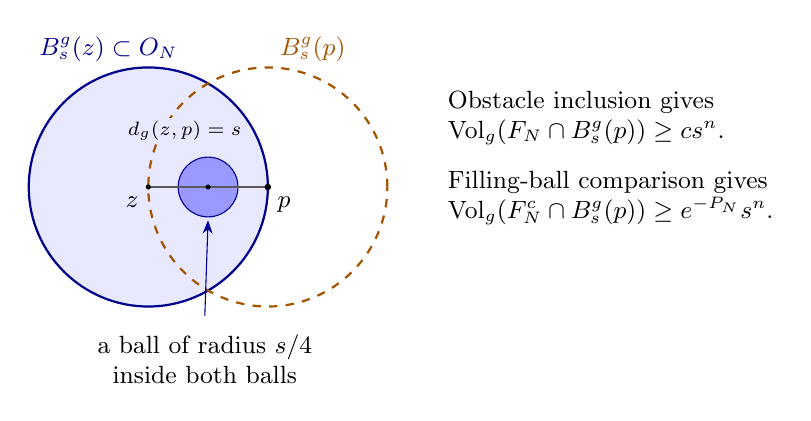
\begin{tikzpicture}[scale=0.92,>=Stealth,
  every node/.style={font=\small}]
  \fill[blue!9] (0,0) circle[radius=1.65];
  \draw[blue!55!black,thick] (0,0) circle[radius=1.65];
  \draw[orange!65!black,thick,dashed] (1.65,0) circle[radius=1.65];
  \fill[blue!40] (0.825,0) circle[radius=0.4125];
  \draw[blue!60!black] (0.825,0) circle[radius=0.4125];
  \draw[black!65] (0,0)--(1.65,0);
  \node[font=\scriptsize,fill=blue!9,inner sep=1pt] at (0.50,0.78) {$d_g(z,p)=s$};
  \fill (0,0) circle[radius=0.035] node[below left] {$z$};
  \fill (0.825,0) circle[radius=0.035];
  \fill (1.65,0) circle[radius=0.045] node[below right] {$p$};
  \node[blue!55!black,align=center] at (-0.55,1.90)
    {$B_s^g(z)\subset O_N$};
  \node[orange!65!black] at (2.27,1.90) {$B_s^g(p)$};
  \draw[->,blue!60!black] (0.78,-1.78)--(0.825,-0.46);
  \node[align=center,anchor=north] at (0.78,-1.90)
    {a ball of radius $s/4$\\inside both balls};
  \node[align=left,anchor=west] at (4.0,0.4)
    {Obstacle inclusion gives\\
     $\Vol_g(F_N\cap B_s^g(p))\ge c s^n$.\\[7pt]
     Filling-ball comparison gives\\
     $\Vol_g(F_N^c\cap B_s^g(p))\ge e^{-P_N}s^n$.};
\end{tikzpicture}
\caption{The two densities at a hypothetical contact point
$p\in\supp|D\mathbf1_{F_N}|\cap\partial O_N$, with $z\in C_N^h$ chosen so that $d_g(z,p)=s=s_N$.
The circles depict background metric balls schematically; no regularity
of the obstacle or of the contact is assumed. Their overlap provides
the first density. Minimality provides the second. Relative isoperimetry
then forces perimeter inside the large constant conformal plateau,
contradicting the competitor bound.}
\label{fig:height:two-densities}
\end{figure}


\subsection{The exterior, its full boundary, and its area}

\begin{proof}[Proof of Theorem~\ref{thm:prepared:deformation}]
\smallskip\noindent\textbf{The connected exterior and its curvature region.}

Choose $F_N$ as in Lemma~\ref{lem:height:BV-existence}.  Its frontier
is compact and, by Lemma~\ref{lem:height:detachment}, has positive
distance from $O_N$.  Every sufficiently small variation of the set
near a frontier point remains admissible.  Thus its boundary is locally
perimeter minimizing in the smooth metric $\widetilde g_N$.

We use the regularity theorem for codimension-one minimizing boundaries:
the support of the perimeter measure is a smooth embedded minimal
hypersurface outside a relatively closed set of Hausdorff dimension at
most $n-8$. A directly applicable smooth-ambient formulation is
\cite[Chapter~7, Section~5, Theorem~5.8]{SimonGMT}; its hypersurface
dimension is $k=n-1$, so the singular bound is $k-7=n-8$.
Multiplicity one for the boundary of a set is recorded in
\cite[Chapter~7, Section~5, Remark~5.2]{SimonGMT}. The compactness and
tangent-cone conclusions used in the minimizing-boundary regularity
argument are Theorems~5.3 and~5.5 of that section.

We also specify the representative of the filled set. Since the
frontier is detached from the obstacle, both insertion and deletion
of a sufficiently small ball are admissible. The coarea and
isoperimetric argument used in the preceding lemma, now applied to
each side, gives positive lower volume densities for both $F_N$ and
its complement at every point in the support of perimeter. On a ball
not meeting that support the indicator has zero distributional
derivative, hence is constant almost everywhere. Let $U_N$ be the
union of those balls on which that constant is zero, and let the
closed filled representative be $\mathcal M_N\setminus U_N$.
The two density bounds identify its topological frontier with the
perimeter support: every neighborhood of a support point contains
both filled and unfilled points. Conversely a point outside the
support has a constant-indicator neighborhood. This representative
agrees with $F_N$ up to a null set; the regularity theorem makes its
frontier $n$-dimensional-volume null. Its perimeter and all the
preceding minimizing comparisons are therefore unchanged.

Put $\Sigma_N=\partial U_N$.
There is only one component of $U_N$.  Indeed there is exactly one
unbounded component, since $F_N$ is bounded and the ambient manifold
has just one end.  Filling all bounded complementary components cannot
increase perimeter.  This statement can be seen directly on regular
boundary charts, where it deletes the separating sheets and adds no
sheet; the singular set has zero $\mathcal H^k$ measure.  Equivalently
it is the component decomposition and perimeter additivity for
finite-perimeter sets \cite{AFP}.  The resulting set is still an
admissible bounded competitor.  If any bounded open component existed,
its positive volume would strictly increase the filled volume; minimality
would either be contradicted by a perimeter decrease or preserved with
a volume increase.  Both alternatives contradict the choice of $F_N$.
Thus $U_N$ is connected.  We take $X_N=\overline{U_N}$, with its
ambient boundary included.

The exterior lies in $\Omega\cap\{|h|<b_3\}$, because the filled
set contains $O_N\supset C_N^h$.  In fact it has a smooth ambient
neighborhood in that region: detachment gives positive separation
between $\Sigma_N$ and $O_N$, and compactness permits a smooth compact
domain containing $O_N$ whose boundary is still strictly inside the
filled set.  Remove that domain.  On the remaining smooth ambient
exterior, Lemma~\ref{lem:height:curvature} gives nonnegative scalar
curvature, also on a neighborhood of $\Sigma_N$.

All local variations of $\Sigma_N$ have zero first variation.  More
precisely, if $Y$ is a compactly supported smooth ambient vector field
near the frontier and $\Phi_s$ is its flow, then $\Phi_s(F_N)$ remains
admissible for both signs of small $s$.  Differentiation of the perimeter
area formula gives
\begin{equation}\label{eq:height:weak-minimality}
 \int_{\partial^*F_N}\divg_{T_x\partial^*F_N}Y\,
 d\mathcal H^k_{\widetilde g_N}=0.
\end{equation}
This is stationarity of the full boundary varifold, including the
assertion that there is no additional first-variation term at the
singular set.  Global outer minimization follows because every bounded
superset of $F_N$ also contains $O_N$.  The maximal choice of $F_N$
also makes it the outermost member among enclosures with this same
minimum perimeter, although outermostness is not required below.

\smallskip\noindent\textbf{Comparison with full original cuts.}\par\nopagebreak[4]

We verify the comparison with original full cuts in some detail.
Detachment and Lemma~\ref{lem:height:ramp} put $\Sigma_N$ in
$\operatorname{int}\Omega$, separated from a neighborhood of the
entire original filling, including every component of $S$.  There are
bounded smooth open sets $F_j$ in the filled manifold such that
\begin{equation}\label{eq:height:strict-approximation}
 \mathbf1_{F_j}\longrightarrow\mathbf1_{F_N}\text{ in }L^1,
 \qquad P_g(F_j)\longrightarrow P_g(F_N),
\end{equation}
and each $F_j$ still contains a fixed neighborhood of the whole filling.
Here is a way to impose the last condition in strict BV approximation.
Choose a smaller compact neighborhood on which $\mathbf1_{F_N}=1$
almost everywhere, separated from $\Sigma_N$, and a compact exterior
region where it is zero.  Smooth the characteristic function in finitely
many coordinate charts only in the remaining region, using a partition
of unity and leaving those two constant regions fixed.  The resulting
smooth functions $u_j\in[0,1]$ converge in $L^1$ with total variation
converging to $P_g(F_N)$.  Choose $\delta_j\downarrow0$ so slowly that
$\|u_j-\mathbf1_{F_N}\|_{L^1}/\delta_j\to0$.  By coarea there is a
regular value $t_j\in(\delta_j,1-\delta_j)$ for which
\[
 P_g(\{u_j>t_j\})
 \le\frac{\int|du_j|_g\,dV_g}{1-2\delta_j}+o(1)
 =P_g(F_N)+o(1).
\]
The $L^1$ difference of this level set from $F_N$ is at most
$\|u_j-\mathbf1_{F_N}\|_{L^1}/\delta_j$, and hence tends to zero.
Lower semicontinuity gives the reverse perimeter liminf.  Thus
$F_j=\{u_j>t_j\}$ satisfies
Equation~\eqref{eq:height:strict-approximation}.  This is the strict
approximation/coarea construction of \cite{AFP}, localized away from
the two constant regions.

For each $j$ retain the component of $\mathcal M_N\setminus\overline{F_j}$
that contains the distant end, and let $D_j$ be its closure.  A compact
smooth boundary has finitely many components; retaining this exterior
component merely selects some of those entire boundary components.
It preserves smoothness and can only decrease the full boundary area.
Because $F_j$ contains a neighborhood of the whole filling,
$D_j\subset\Omega$, its interior lies in $\operatorname{int}\Omega$,
and $D_j$ is closed and connected with a smooth compact intrinsic
boundary $\Gamma_j$.  It is an admissible full cut in
Definition~\ref{def:fullcuts}.  Thus
\[
 a\le\Area_g(\Gamma_j)\le P_g(F_j).
\]
Taking the limit gives $P_g(F_N)\ge a$.  No component of a cut has
been discarded in evaluating its intrinsic boundary; the passage to
$D_j$ is an admissible choice of the exterior domain itself.  There is
no coincidence with $S$ in this approximation because of the fixed
neighborhood, and the original definition still allows coincidence for
its other competitors.

Since $\widetilde g_N\ge e^{-2\epsilon}g$ on $\Omega$, comparison
on every approximate tangent $k$-plane now yields
\begin{equation}\label{eq:height:original-area}
 \mathcal H^k_{\widetilde g_N}(\Sigma_N)
 =P_{\widetilde g_N}(F_N)
 \ge e^{-k\epsilon}P_g(F_N)\ge e^{-k\epsilon}a.
\end{equation}
The first equality uses the regularity theorem and the zero
$\mathcal H^k$ measure of the singular set.

\smallskip\noindent\textbf{Completeness and the end.}

The filled metric is complete, since
$\widetilde g_N\ge e^{-2\epsilon}g$ and the background filled metric
is complete.  Its restriction to $X_N$ is complete with the frontier
included.  Here completeness is understood in the enclosing-set
convention of the Riemannian input: the intrinsic length distance on
$X_N$ may be extended-valued, and its restriction to each finite-distance
equivalence class is complete.  For the intrinsic-length formulation, a Cauchy sequence
has a subsequence whose successive intrinsic distances are less than
$2^{-j}$.  Join successive terms by curves of length less than
$2^{1-j}$ in $X_N$.  Their concatenation has an ambient endpoint,
by ambient completeness, and that endpoint belongs to $X_N$ because
$X_N$ is closed.  Appending this endpoint gives a curve in $X_N$
whose tail length tends to zero, proving intrinsic convergence of the
subsequence and then of the original Cauchy sequence.  The frontier
is included in the closed-enclosing-set sense used in
the Riemannian input in Section~\ref{sec:comparison}.

Finally the end satisfies $\widetilde g_N-I=O_j(r^{2-n})$.
The conformal law applied to Equation~\eqref{eq:height:end-input}
shows
\[
 R_{\widetilde g_N}=O(r^{-n-\beta})+O(r^{-2n+2}).
\]
If needed decrease $\beta$ so that $0<\beta<n-2$; then the displayed
bound is $O(r^{-n-\beta})$.  All graph errors decay exponentially,
and $\psi_N$ is zero on the end.  Scalar curvature is integrable there
and, being smooth and bounded on the compact ambient neighborhood of
the frontier, integrable on the remainder of $X_N$.
The energy estimate is Lemma~\ref{lem:height:curvature}.  This proves
all the stated properties.
\end{proof}

\begin{remark}[Flux and weak boundary conventions]\label{rem:height:flux}
The scalar flux in Proposition~\ref{prop:scalar:flux} is computed on
the complete smooth filled manifold before an enclosure is chosen:
\[
 \mathfrak F_N=\lim_{R\to\infty}\int_{S_R}g(V,\nu_g)\,dA_g
 =\int_{\mathcal M_N}u\Xi\,dV_g,
 \qquad E(\widehat g)-E=-\frac{\mathfrak F_N}{k\omega}.
\]
Thus no elliptic boundary condition or unaccounted singular-boundary
flux is involved.  If one restricts a smooth vector field to $X_N$,
the Gauss--Green theorem for finite-perimeter sets gives its ordinary
reduced-boundary flux.  For instance at a regular truncation radius,
\[
 \int_{U_N\cap B_R}\divg_{\widetilde g_N}Y\,dV_{\widetilde g_N}
 =\int_{S_R}\widetilde g_N(Y,\nu_R)\,dA_{\widetilde g_N}
 -\int_{\partial^*F_N}\widetilde g_N(Y,\nu_{F_N})\,
 dA_{\widetilde g_N},
\]
when $Y$ is supported in the indicated truncation or has its stated
outer trace.  The normal $\nu_{F_N}$ points from the filled set toward
the end.  There is no further measure on the singular set.  This flux
convention and Equation~\eqref{eq:height:weak-minimality} are the weak
identities attached to the constructed boundary.
\end{remark}

\section{Weakly asymptotically flat data in three dimensions}
\label{sec:weak3}\label{n3:intro:section}\label{n3:reduction:section}

The prepared theorem can be applied under only two differentiated metric
bounds and one differentiated tensor bound in dimension three. The reason
is a separate end construction: first match the original ADM vector by a
Schwarzschild reference slice, then bend that slice to rest and repair the
small constraint error. The metric changes at distances tending to infinity.
We prove compactness of minimizing enclosures before making those changes;
it gives convergence of the full enclosing infimum, not only a one-sided
area bound. A positive conformal family subsequently removes timelikeness
as an assumption, and truncation of the other ends gives the complete-data
statement.

\subsection{Initial data, normals, and enclosing area}

We work in three spatial dimensions, with zero cosmological constant and
\(G=c=1\). In this section $\mu,J$ denote the physical densities:
the geometric densities of Equation~\eqref{eq:setting:constraints} are
$8\pi\mu,8\pi J$. The ADM energy and momentum retain exactly their
previous normalization. We spell out this dictionary again when applying
the common prepared theorem. For a Riemannian metric \(g\) and a symmetric covariant
two-tensor \(K\), define the constraint densities by
\begin{equation}\label{n3:intro:constraints}
 16\pi\mu=R_g+(\tr_gK)^2-|K|_g^2,\qquad
 8\pi J=\Div_g\bigl(K-(\tr_gK)g\bigr).
\end{equation}
Here \(J\) is a covector field. The dominant energy condition is
\begin{equation}\label{n3:intro:dec}
                         \mu\ge |J|_g.
\end{equation}
All initial data considered here are smooth, including at a compact
boundary when one is present.

On an asymptotically flat end with Euclidean coordinates \(x\) and
\(r=|x|\), our basic assumptions are
\begin{equation}\label{n3:intro:decay}
 g_{ij}-\delta_{ij}=O_2(r^{-q}),\qquad
 K_{ij}=O_1(r^{-1-q}),\qquad q>\tfrac12.
\end{equation}
The notation \(O_j(r^{-a})\) includes the corresponding coordinate
derivative bounds through order \(j\). We assume that \(\mu\) and
\(|J|_g\) are integrable and that the following ADM limits exist and are
finite:
\begin{align}
 E&=\frac1{16\pi}\lim_{r\to\infty}
   \int_{S_r}(\partial_jg_{ij}-\partial_i g_{jj})n^i
                    \dd A_\delta,\label{n3:intro:energy}\\
 P_i&=\frac1{8\pi}\lim_{r\to\infty}
   \int_{S_r}\bigl(K_{ij}-(\tr_gK)g_{ij}\bigr)n^j
                    \dd A_\delta.\label{n3:intro:momentum}
\end{align}
The normal and area form in these definitions are Euclidean. Whenever
\(E>|P|_\delta\), write
\begin{equation}\label{n3:intro:rest-mass}
                         m=\sqrt{E^2-|P|_\delta^2}.
\end{equation}

For a two-sided surface \(\Sigma\) with specified unit normal \(\nu\),
we use
\[
 H_\Sigma=\Div_\Sigma\nu,\qquad
 \theta_+(\Sigma)=H_\Sigma+\tr_\Sigma K.
\]
Thus Euclidean spheres have positive mean curvature for the normal
toward infinity. A future marginally outer trapped surface, abbreviated
MOTS, satisfies \(\theta_+=0\). A weakly future outer trapped surface
satisfies \(\theta_+\le0\). Our spacetime sign convention is
\begin{equation}\label{n3:intro:k-sign}
 K(Y,Z)=\mathbf g(\mathbf\nabla_Y n,Z),
\end{equation}
where \(n\) is the future unit timelike normal. Equivalently, in Gaussian
normal coordinates the spatial metric has normal derivative \(2K\).

\begin{definition}[Exterior and enclosing area]\label{n3:intro:exterior-class}
An exterior is a connected orientable smooth three-manifold \(\Omega\)
with nonempty compact smooth boundary, complete as a metric space with
its boundary included, and with exactly one end, which is asymptotically flat.
An enclosing cut is the entire compact smooth embedded two-sided intrinsic
boundary of a connected closed outer domain containing the sufficiently
distant end, with its manifold interior in the open exterior. Equivalently,
it separates the entire inner boundary from infinity, with bounded
complementary pockets filled on the inner side. Every frontier component is
counted, including portions coinciding with the inner boundary. A cut may
have several components. Its normal points toward the retained end. We put
\[
 a_g(\partial\Omega)=
  \inf\{|\Gamma|_g:\Gamma\text{ is an enclosing cut}\}.
\]
When using perimeter compactness, we take the closure of this class
among filled inner sets and include the area of any frontier coinciding
with the obstacle. Smooth outward approximation gives the same
infimum. Enclosing cuts and minimizing sets are taken with bounded
complementary pockets filled. Auxiliary perimeter arguments may use
competitors containing the inner obstacle before filling: filling a bounded
pocket deletes its frontier, cannot increase perimeter, and leaves the enclosing
infimum unchanged.
\end{definition}

The definition permits coincidence because first variations of the
minimum need not be realized by a cut lying strictly outside the
obstacle. It permits disconnected cuts because neither the minimizing
hull nor an intermediate trapped boundary need be connected. The
perimeter formulation and its compactness properties are established
in Lemma~\ref{n3:reduction:area-compactness}.

\subsection{The one-ended exterior inequality}

\begin{theorem}[Minimum-enclosing-area inequality]\label{n3:intro:exterior-inequality}
Let \((\Omega,g,K)\) be an exterior as in
Definition~\ref{n3:intro:exterior-class}. Assume
Equations~\eqref{n3:intro:constraints}--\eqref{n3:intro:decay}, integrability
of \(\mu\) and \(|J|_g\), and the finite ADM limits
\eqref{n3:intro:energy}--\eqref{n3:intro:momentum}. Orient \(\partial\Omega\)
by the normal into \(\Omega\), and suppose
\(\theta_+(\partial\Omega)\le0\). If \(E>|P|_\delta\), then
\begin{equation}\label{n3:intro:penrose}
          \sqrt{E^2-|P|_\delta^2}
               \ge \sqrt{\frac{a_g(\partial\Omega)}{16\pi}}.
\end{equation}
No extension of the data across \(\partial\Omega\) is required.
\end{theorem}


\subsection{A positive lower bound for every enclosing cut}

Before preparing the end, we record a geometric fact about the full
enclosing infimum. A thin tube joining the inner boundary to infinity
carries a fixed flux through every enclosing cut. A bound for the
flux density then gives a uniform positive area bound. This argument
uses neither the constraint equations nor a sign for the boundary
expansion.

\begin{lemma}[Positive enclosing area]
\label{bridge:bridge:positive-area}
Let $(\Omega,g)$ be a connected orientable smooth three-dimensional exterior,
complete with its nonempty compact smooth boundary $B$ included, with
one asymptotically flat end and compact complement. Let $a_g(B)$ be
the infimum of the full areas of the enclosing cuts in
Definition~\ref{n3:intro:exterior-class}, including all components and
all portions coincident with $B$. Then
\[
                         0<a_g(B)<\infty.
\]
\end{lemma}

\begin{proof}
A sufficiently large coordinate sphere encloses $B$, so the infimum
is finite. To obtain a lower bound, choose a point of $B$ and a smooth
proper embedded ray starting there, initially normal to $B$ and pointing
into $\Omega$. Choose the ray to be straight in the asymptotic coordinates
outside a compact set. A tubular neighborhood has product coordinates
$(t,y)\in[0,\infty)\times D^2$, with its initial disk contained in $B$.
On the straight tail the transverse coordinate disk can have a fixed
positive width.

Choose a smooth two-form $\eta$ supported in the interior of $D^2$ with
$\int_{D^2}\eta=1$. Pull it back by $(t,y)\mapsto y$ and extend it by
zero across the lateral boundary of the tube. This gives a smooth
closed two-form $\omega$ on $\Omega$, smooth also at $B$. Its pointwise
comass is bounded: this follows from compactness on the initial portion
of the tube and from asymptotic flatness and fixed coordinate width on
the tail. Write
\[
 C_\omega=\sup_{x\in \Omega}\sup_{
       v,w\ \text{orthonormal in }(T_x\Omega,g)}|\omega_x(v,w)|<\infty.
\]
Orient the transverse disk so that the flux through a sufficiently
large outward-oriented coordinate sphere $S_R$ is one.

Let $\Gamma$ be a smooth enclosing cut lying in the interior of $\Omega$,
oriented toward the end, and choose $S_R$ outside it. The region between
$\Gamma$ and $S_R$ is compact and disjoint from $B$; all of its inner
boundary components are counted in $\Gamma$. Stokes' theorem gives
\[
       \int_\Gamma\omega=\int_{S_R}\omega=1,
       \qquad 1\le C_\omega\operatorname{Area}_g(\Gamma).
\]
This calculation also applies when the cut is disconnected. If a
smooth cut touches or coincides with $B$, push it into the interior
by a smooth collar flow pointing from $B$ into $\Omega$, filling the collar on the obstacle
side. The resulting surfaces are enclosing cuts and their areas
converge to the full area of the original cut. Thus the same lower
bound holds for boundary-coincident cuts. Taking the infimum yields
$a_g(B)\ge C_\omega^{-1}>0$. The smooth/perimeter equivalence in the
definition of the full enclosing infimum transfers this bound to its
filled-perimeter formulation as well.
\end{proof}

Throughout the construction, write $B=\partial\Omega$.
Thus $\Omega$ is smooth, connected and orientable, complete including its
nonempty compact smooth boundary, and has a single Euclidean coordinate
end with compact complement. The boundary normal points into $\Omega$.
The differentiated asymptotic assumptions are
\begin{equation}\label{n3:reduction:original-decay}
 g-\delta=O_2(r^{-q}),\qquad K=O_1(r^{-1-q}),\qquad q>\tfrac12.
\end{equation}
The density, finite-charge and weak-trapping hypotheses are those stated
in Theorem~\ref{n3:intro:exterior-inequality}. The preparation assumes
$E>|P|$; the conformal construction immediately below does not.

\subsection{A strict conformal direction}

Conformal strictification by a spacetime Poisson equation was developed
by Jaracz~\cite{Jaracz2025StrictDEC}. Here a regularized drift equation
with nonzero inner Neumann data also gives strict trapping, an exact
energy slope, unchanged momentum, and comparison of all enclosing cuts.
These quantitative conclusions are established below.

\begin{lemma}[Conformal constraint formulas]
\label{n3:reduction:conformal-formulas}
For a smooth function $f$, set
\[
 g_f=e^{4f}g,\qquad K_f=e^{2f}K.
\]
The corresponding constraint densities satisfy
\begin{align}
 16\pi e^{4f}\mu_f
   &=16\pi\mu-8\Delta_g f-8|df|_g^2,
       \label{n3:reduction:conformal-energy}\\
 8\pi J_f
   &=e^{-2f}\bigl(8\pi J+4K(\nabla f,\cdot)\bigr).
       \label{n3:reduction:conformal-momentum}
\end{align}
Here the second identity is an identity of covectors.  Consequently,
\begin{align}
 16\pi e^{4f}(\mu_f-|J_f|_{g_f})
 \ge{}&16\pi(\mu-|J|_g)\notag\\
 &+8\bigl(-\Delta_g f-|df|_g^2-|K|_g|df|_g\bigr).
       \label{n3:reduction:conformal-dec}
\end{align}
On the fixed boundary,
\begin{equation}
 \theta_{+,f}=e^{-2f}(\theta_++4\partial_\nu f).
       \label{n3:reduction:conformal-expansion}
\end{equation}
Equivalently, if $u=e^f>0$, the last summand in
Equation~\eqref{n3:reduction:conformal-dec} is
$8u^{-1}(-\Delta_g u-|K|_g|du|_g)$.
\end{lemma}

\begin{proof}
Apply the pointwise identities in Equation~\eqref{eq:end:conformal}
with $n=3$, $k=2$, $p=1$, and $s=2f$. The densities in that identity
are $\mu_{\mathrm A}=8\pi\mu$ and $J_{\mathrm A}=8\pi J$ in this
section's physical normalization. Setting the vector argument to zero
gives $8\pi e^{4f}\mu_f=8\pi\mu-4\Delta f-4|df|^2$;
multiplication by two is
Equation~\eqref{n3:reduction:conformal-energy}. The covector formula
proved there gives
$8\pi J_f=e^{-2f}(8\pi J+4K(\nabla f,\cdot))$.
Its new-metric norm introduces a further factor $e^{-2f}$, so the
triangle inequality gives Equation~\eqref{n3:reduction:conformal-dec}
with precisely its factor $8$. The boundary formula has
$k\partial_\nu s=4\partial_\nu f$ and proves
Equation~\eqref{n3:reduction:conformal-expansion}. Finally
Equation~\eqref{eq:end:conformal-U} uses $U=e^f=u$ here and gives
the stated positive-factor form. These are pointwise identities;
no decay or additional differentiated end hypothesis is used.
\end{proof}

\begin{lemma}[Strict direction under the original decay]
\label{n3:reduction:strict-direction}
Choose
\[
 0<\delta<\beta<\min(q,1).
\]
There are smooth positive functions $w$ and $\phi$ on $\Omega$, with
$w=r^{-3-\delta}$ on the end, such that
\begin{align}
 &\partial_\nu\phi=-1\quad\hbox{on }B,
       &\phi&=O_2(r^{-1}),\label{n3:reduction:strict-boundary}\\
 &-\Delta_g\phi-|K|_g|d\phi|_g\ge w,
       &\frac{-\Delta_g\phi}{w}&\longrightarrow1.
       \label{n3:reduction:strict-source}
\end{align}
The Euclidean normal flux
\[
 L_\phi=\lim_{r\to\infty}
          \int_{S_r}\partial_r\phi\,\dd A_\delta
\]
is finite and negative.  For every finite $s\ge0$, set
\begin{equation}
 \label{n3:reduction:linear-family}
 u_s=1+s\phi,\qquad g_s=u_s^4g,\qquad K_s=u_s^2K.
\end{equation}
These data are complete up to $B$ and satisfy DEC, strictly for $s>0$.
If $\theta_+\le0$ on $B$, their boundary expansion remains nonpositive
and is strictly negative for $s>0$.  Their decay exponent can be taken to be
$\min(q,1)>1/2$, their constraint densities are integrable, and
\begin{equation}
 \label{n3:reduction:strict-charges}
 E_s=E+sA_\phi,\qquad P_s=P,
 \qquad A_\phi=-\frac{L_\phi}{2\pi}>0.
\end{equation}
Their full enclosing infima satisfy
\begin{equation}
 \label{n3:reduction:strict-areas}
 a_g(B)\le a_{g_s}(B)
       \le (1+s\|\phi\|_\infty)^4a_g(B).
\end{equation}
In particular $E_s\to E$ and $a_{g_s}(B)\to a_g(B)$ as $s\downarrow0$.
No sign assumption on the ADM vector is needed.

If $K$ is compactly supported and the metric has symbol estimates of all
orders with $g-\delta=O(r^{-1})$, the function can instead be chosen with
$\phi=O_k(r^{-1})$ for every $k$, while retaining
Equations~\eqref{n3:reduction:strict-boundary} and
\eqref{n3:reduction:strict-source}.
\end{lemma}

\begin{proof}
Choose smooth $b\ge|K|_g$, positive everywhere and equal to
$b_0r^{-1-\beta}$ sufficiently far out, where $b_0>0$ is chosen large
enough.  This is possible because $\beta<q$.  Choose a smooth positive
regularizer $\zeta$, equal to $r^{-2}$ on the end, and extend $w$ smoothly
and positively to $\Omega$.  We solve
\begin{equation}
 \label{n3:reduction:drift-poisson}
 -\Delta_g\phi=b\sqrt{|d\phi|_g^2+\zeta^2}+w,
 \qquad \partial_\nu\phi=-1,
 \qquad \phi\longrightarrow0.
\end{equation}
The regularizer makes this equation smooth even at critical points.

First truncate at a large coordinate sphere $S_R$ and prescribe
$\phi=0$ there.  The Neumann and Dirichlet conditions occur on disjoint
boundary components.  For $0\le t\le1$, replace $b$ in
Equation~\eqref{n3:reduction:drift-poisson} by $tb$.  At $t=0$, the mixed
Laplacian is invertible: its Dirichlet face gives the Poincare inequality,
and the weak solution obtained from its coercive quadratic form is smooth
by boundary regularity.  At any solution, the linearization is a
Laplacian with a smooth drift of norm at most $b$ and with the homogeneous
mixed boundary conditions.  The strong maximum principle and the Hopf
boundary principle make its kernel zero.  It is a Fredholm perturbation
of the mixed Laplacian of index zero, and is therefore invertible.
The boundary estimates used here are the ordinary elliptic estimates
for Dirichlet and normal Neumann conditions: positive definiteness of
$g$ verifies their principal complementing condition, and the disjoint
boundary components can be covered separately
\cite{AgmonDouglisNirenberg1959}.  The maximum principles and local
elliptic estimates below are used in their usual uniformly elliptic
forms \cite{GilbargTrudinger}.

To close continuation at $t=1$, first work on a fixed truncation.
The elliptic $W^{2,p}$ estimate
and gradient interpolation give
\[
 \|\phi\|_{W^{2,p}}
 \le C_p\bigl(1+\|\phi\|_{L^p}+\|d\phi\|_{L^p}\bigr)
 \le \tfrac12\|\phi\|_{W^{2,p}}
       +C'_p(1+\|\phi\|_{L^p}).
\]
The constants include the fixed boundary data and are uniform in $t$.
If the supremum norms of solutions on this truncation were unbounded,
divide them by their supremum norms.  The preceding estimate with
$p>3$, compactness, and the equation give a nonzero limit $v$ with
homogeneous mixed data satisfying
\[
 -\Delta_gv=t_*b|dv|_g.
\]
This can be written $\Delta_gv+A\cdot dv=0$ with a bounded measurable
drift: take $A=t_*b\nabla v/|dv|$ off the critical set and zero on it.
The strong and Hopf maximum principles exclude a nonzero solution with
the homogeneous mixed conditions.  Thus the supremum norms are bounded.
The $W^{2,p}$ estimate, Schauder estimates, and the smooth equation now
give the bounds needed for closedness of continuation.  Existence on
each truncation follows.

Every such solution is nonnegative.  A negative minimum cannot be
interior because the right side of
Equation~\eqref{n3:reduction:drift-poisson} is positive.  At an inner-boundary
minimum, the outward-domain derivative would be negative by the Hopf
principle, whereas the prescribed derivative in that direction is $1$.
The outer value is zero.

It remains to make these bounds independent of $R$.  For fixed sufficiently large
$A$ and then sufficiently large $r_0$, the positive radial function
\[
 v_0(r)=r^{-1}(1-Ar^{-\delta})
\]
satisfies, on $r\ge r_0$,
\begin{align*}
 -\Delta_gv_0-b|dv_0|_g
 &=A\delta(1+\delta)r^{-3-\delta}
       +O(r^{-3-q})+O(r^{-3-\beta})\ge c_0w.
\end{align*}
The constants are fixed independently of the truncation.  Since
$b\zeta=o(w)$, a sufficiently large multiple of $v_0$ is a supersolution
of the regularized equation.  The comparison principle gives
\begin{equation}
 \label{n3:reduction:core-barrier}
 0\le\phi(x)\le C(1+M_R)v_0(r),\qquad
 M_R=\sup_{\Omega\cap\{r\le r_0\}}\phi,
 \quad r_0\le r\le R.
\end{equation}
The notation for the compact core includes all points outside the end
chart.  Were $M_R$ unbounded along expanding truncations, the normalized
solutions $\phi/M_R$ would have locally uniform $W^{2,p}$ bounds, including
at $B$, by the preceding local estimates and
Equation~\eqref{n3:reduction:core-barrier}.  A subsequence would converge
locally in $C^1$ to a nonnegative function with maximum one on the core,
homogeneous inner Neumann data, and a bounded-drift homogeneous equation.
Equation~\eqref{n3:reduction:core-barrier} makes its value tend to zero at
infinity.  It consequently attains a positive maximum, contradicting the
strong or Hopf principle for that homogeneous equation.  This proves the
uniform core bound.  The contradiction uses the homogeneous bounded-drift
equation.

Local compactness and diagonal extraction give a smooth solution of
Equation~\eqref{n3:reduction:drift-poisson}, with $\phi=O(r^{-1})$.
The claimed derivative count can be checked directly on annuli.  Put
\[
 \phi_{\rho}(y)=\rho\phi(\rho y),\qquad
 g_{\rho}(y)=g(\rho y),\qquad 1<|y|<4.
\]
On smaller fixed annuli the equation is
\[
 -\Delta_{g_{\rho}}\phi_{\rho}
 =\rho b(\rho y)
       \sqrt{|d\phi_{\rho}|_{g_{\rho}}^2+
                     (\rho^2\zeta(\rho y))^2}
       +\rho^3w(\rho y).
\]
Its coefficients have uniform $C^{1,1}$ bounds from the two derivatives
in Equation~\eqref{n3:reduction:original-decay}; the scaled drift is
$O(\rho^{-\beta})$ and the scaled source is $O(\rho^{-\delta})$.
The bounded zeroth-order norm, interior $W^{2,p}$ estimates, and gradient
interpolation first give uniform $C^{1,\alpha}$ bounds for some
$\alpha>0$.  The right side is then uniformly $C^\alpha$.  Schauder
estimates give uniform $C^{2,\alpha}$ bounds on smaller annuli.  This
proves $\phi=O_2(r^{-1})$ without using a third derivative of $g$ or a
second derivative of $K$.

The right side of Equation~\eqref{n3:reduction:drift-poisson} is
$w+O(r^{-3-\beta})$.  It is integrable and proves
Equation~\eqref{n3:reduction:strict-source}.  The divergence theorem, with
outward-domain normal $-\nu$ on $B$, gives
\begin{equation}
 \label{n3:reduction:phi-flux}
 \lim_{r\to\infty}\int_{S_r}\partial_{n_g}\phi\,\dd A_g
 =-|B|_g-\int_{\Omega}
       \bigl(b\sqrt{|d\phi|_g^2+\zeta^2}+w\bigr)\,\dd V_g.
\end{equation}
The Euclidean flux differs by $O(r^{-q})$ and has the same finite limit.

For every fixed finite $s\ge0$, the factor $u_s$ in
Equation~\eqref{n3:reduction:linear-family} is bounded and at least one,
so the transformed data are complete up to $B$.
The $u$-form of Lemma~\ref{n3:reduction:conformal-formulas} gives
\begin{align*}
 16\pi u_s^4(\mu_s-|J_s|_{g_s})
 &\ge16\pi(\mu-|J|_g)
        +\frac{8s}{u_s}(-\Delta_g\phi-|K|_g|d\phi|_g)
 \ge \frac{8s}{u_s}w,\\
 \theta_{+,s}
 &=u_s^{-2}\left(\theta_+-\frac{4s}{u_s}\right).
\end{align*}
This proves the asserted signs for all finite $s$, without a smallness
restriction.

Since $u_s-1=O_2(r^{-1})$, the transformed decay exponent is
$\min(q,1)>1/2$.  The exact energy transformation is
\[
 16\pi u_s^4\mu_s=16\pi\mu-8s u_s^{-1}\Delta_g\phi.
\]
Here $\Delta_g\phi=O(r^{-3-\delta})$, and the additional current term
is bounded by a fixed-$s$ constant times
$|K|_g|d\phi|_g=O(r^{-3-q})$.  Both are integrable in dimension three.
The bounded positive conformal factor also preserves integrability in
the transformed volume measure.

The leading metric change is $4s\phi\delta$, whose ADM energy flux
is $-8s\int_{S_r}\partial_r\phi\,\dd A_\delta$ before division by
$16\pi$.  All remaining metric flux terms are
$O_s(r^{-q})+O_s(r^{-1})$.  Writing $\pi=K-(\tr_gK)g$, one has
$\pi_s=u_s^2\pi$, so the change in its Euclidean momentum flux is
$O_s(r^2r^{-1}r^{-1-q})=O_s(r^{-q})$.
This proves Equation~\eqref{n3:reduction:strict-charges};
Equation~\eqref{n3:reduction:phi-flux} gives $A_\phi>0$.
No $1/r$ coefficient expansion for $\phi$ is needed.
Finally, the cut class is unchanged and every cut has area
$\int_\Gamma u_s^4\,\dd A_g$.  Bounding $u_s$ between $1$ and
$1+s\|\phi\|_\infty$ and taking infima proves
Equation~\eqref{n3:reduction:strict-areas}, including coincident and
disconnected cuts.

For the final assertion, take $b$ nonnegative, compactly supported, and
at least $|K|$; the proof is unchanged.  The end equation is then simply
$-\Delta_g\phi=w$.  Once the two-derivative estimate has been established,
successive annular elliptic estimates use the assumed symbol bounds for
$g$ and $w$ to give $\phi=O_k(r^{-1})$ for every $k$.
\end{proof}

\subsection{Compactness of enclosing minimizers}

The end replacement will change the metric on receding annuli.  The next
lemma keeps area-minimizing enclosures in a fixed compact set, where local
metric convergence controls their areas.

\begin{lemma}[Enclosing areas under receding changes]
\label{n3:reduction:area-compactness}
Let $g_j$ be smooth metrics on the fixed exterior $\Omega$, converging to $g$
locally uniformly up to $B$.  Suppose that in a fixed chart outside a
compact set they satisfy, with constants independent of $j$,
\begin{equation}
 \label{n3:reduction:area-geometry}
 c\delta\le g_j\le C\delta,\qquad r|\partial g_j|_\delta\le C.
\end{equation}
Suppose also that each $g_j$ has an asymptotically flat end, possibly
in a different chart, and admits a fixed compact enclosing competitor
with uniformly bounded area.  Then minimizing filled enclosures exist,
their boundaries lie in one fixed compact subset of $\Omega$, and
\[
 a_{g_j}(B)\longrightarrow a_g(B).
\]
The perimeter and smooth enclosing infima agree.  Each minimizing
boundary is $C^{1,1}$, and is smooth minimal away from contact with $B$.
\end{lemma}

\begin{proof}
For purposes of perimeter minimization only, extend the metrics through
a collar of $B$ and attach a fixed compact filling.  The filling need not
satisfy any constraint or curvature condition.  Extend $g_j$ so that the
extensions converge uniformly on this fixed collar and filling.  A filled
enclosure is then a bounded set containing the prescribed inner obstacle.

For each fixed metric, sufficiently large spheres in its asymptotically
flat chart have strictly positive outward mean curvature.  Clipping a
bounded enclosure at any such sphere cannot increase perimeter.  To see
this, integrate the divergence of the outward unit normal field of the
sphere foliation over the part of the enclosure outside the sphere.  Its
divergence is positive.  Its flux through the exterior boundary is at
most the area of that boundary, whereas its flux on the cutting sphere
is the negative of the new cutting area.  Thus the discarded boundary
area is at least the inserted area.  Approximation gives the same
statement for finite-perimeter sets.  The direct method on the resulting
bounded domain now gives a minimizer.  The clipping observation makes
this a minimizer against every bounded competitor, not merely those
inside the chosen truncation.

Off the obstacle the boundary is locally perimeter minimizing.  If it
contains a point of radius $r$ sufficiently large, the coordinate ball
of radius $c_1r$ about that point avoids the obstacle.  After scaling
this ball to unit size, Equation~\eqref{n3:reduction:area-geometry} gives
uniform ellipticity and uniform first-derivative bounds for its area
integrand.  The local perimeter density estimate gives
\[
 \operatorname{Area}_{g_j}
       (\partial F_j\cap B_{c_1r})\ge c_2r^2.
\]
Here $c_1,c_2>0$ are independent of $j$ and $r$. To justify the
uniform lower bound, work in a rescaled coordinate ball avoiding the
obstacle, and let $v(s)=|F_j\cap B_s|_\delta$. Removing $F_j\cap B_s$
is an admissible local comparison. For almost every $s$, minimality
and uniform metric comparability give
\[
 P_\delta(F_j;B_s)\le C v'(s),\qquad
 P_\delta(F_j\cap B_s)\le C'v'(s).
\]
The Euclidean isoperimetric inequality therefore yields
$v(s)^{2/3}\le C''v'(s)$. At a point in the support of the minimizing
frontier, both phases meet every ball. Integrating this differential
inequality gives $v(s)\ge c s^3$. Filling the complement in $B_s$
gives the same estimate for $|B_s\setminus F_j|_\delta$. The relative
isoperimetric inequality now gives
$P_\delta(F_j;B_s)\ge c's^2$ on a smaller fixed ball. Returning to
the original scale proves the displayed area bound. The argument also
applies at all support points by taking limits of reduced-boundary
points. No uniform curvature or higher metric derivative bound is used.
The fixed competitor bounds the total area independently of $j$.
Consequently the minimizing boundaries lie in a fixed compact set.

The local obstacle regularity theorem for pure area minimization with
a $C^2$ obstacle gives $C^{1,1}$ regularity, and smoothness off contact,
in dimension three; its local estimates require only the appropriate
bounded geometry of the smooth metric
\cite[Regularity Theorem 1.3]{HuiskenIlmanen2001}.
This applies to the fixed smooth obstacle and each of the smooth
metrics $g_j$ and $g$ after the collar extension. Push a minimizing
boundary slightly away from its contact set by a smooth vector field agreeing
there with the outward obstacle normal.  In a small obstacle collar its
flow increases the signed distance to the obstacle.  The resulting
$C^1$ embedded boundary is a positive distance from the obstacle.
Smooth local graph approximation, within that distance, preserves
enclosure and changes area by an arbitrarily small amount.  This proves
equality of the smooth and perimeter infima for each metric.

Enlarge the fixed compact region so that its complement is a connected
coordinate tail. Each minimizing inner set is either empty or the whole
tail there, since its frontier is absent. Boundedness excludes the latter,
so the sets themselves also lie in a common compact set.
Choose a fixed smooth auxiliary metric on this compact set. Uniform
metric comparability gives uniformly bounded auxiliary perimeters, and
BV compactness gives a limiting filled enclosure. The obstacle is still
contained in the limit. Fill any newly bounded complementary pockets;
this only removes frontier. Uniform metric convergence makes the area
integrands converge uniformly relative to the auxiliary metric, so lower
semicontinuity implies
\[
 a_g(B)\le\liminf_j a_{g_j}(B).
\]
Conversely, using a fixed enclosure with $g$-area arbitrarily close to
$a_g(B)$ gives the reverse upper-limit inequality.
\end{proof}

\subsection{Schwarzschild reference charges}

The area infimum is now stable under uniformly controlled changes on
receding annuli. We next arrange those changes. The vacuum reference end
must first have the original ADM charges; only after matching can we bend
it to a rest slice without paying a nonvanishing constraint-repair cost.

\begin{lemma}[A reference end with prescribed timelike charges]
\label{n3:reduction:boosted-reference}
Let $E>|P|$ and $m=(E^2-|P|^2)^{1/2}$.  There is a spacelike plane
near spatial infinity of Schwarzschild spacetime of mass $m$ whose
induced data, in asymptotically Euclidean coordinates on the plane,
have ADM charges $(E,P)$.  The reference data satisfy
\[
 g_*-\delta=O_k(r^{-1}),\qquad K_*=O_k(r^{-2})
\]
for every derivative order $k$.
\end{lemma}

\begin{proof}
Apply Lemma~\ref{lem:end:boost} with $n=3$, $k=2$, $p=1$, and
$M=m$. In static isotropic coordinates $(T,y)$ its spacetime metric is
\begin{equation}
 \label{n3:reduction:schwarzschild-spacetime}
 -\left(\frac{1-m/(2r)}{1+m/(2r)}\right)^2\dd T^2
       +\left(1+\frac{m}{2r}\right)^4\delta_{ij}\dd y^i\dd y^j,
 \qquad r=|y|.
\end{equation}
For $P\ne0$, put $v=P/E$ and rotate the boost axis into its direction;
for $P=0$, take $v=0$. Then
$\gamma=(1-|v|^2)^{-1/2}=E/m$, and the reference plane has charges
$(m\gamma,m\gamma v)=(E,P)$. The common lemma uses the same
future-normal convention for $K$, and its ADM prefactors become
\[
 \frac1{2k\omega_2}=\frac1{16\pi},\qquad
 \frac1{k\omega_2}=\frac1{8\pi}.
\]
Thus its charges have precisely the present signs and normalization;
the use of physical constraint densities here does not rescale them.

For the later bend, write the plane as $T=v\cdot y$ and set
$y=Ax$, where $A=(I-v\otimes v)^{-1/2}$. The induced Minkowski
metric in the $x$ coordinates is $\delta$. The perturbation of the
metric above from Minkowski space has symbol decay of order $r^{-1}$
on this fixed spacelike plane, and
Lemma~\ref{lem:end:boost} gives the induced metric and tensor orders
$r^{-1}$ and $r^{-2}$ through every fixed derivative order. These
estimates concern the exact reference end and impose no additional
derivative assumption on the original data.
\end{proof}

\subsection{Moments and compact linear corrections}

The reference end has the required charges, but interpolation can
violate DEC. Compact linear corrections reduce this error before the
conformal repair. This is related to localized constraint deformation
and its adjoint obstructions
\cite{CorvinoSchoen2006,ChruscielDelay2003}; those results are not being
invoked as a no-parity DEC rest-end or all-cut comparison theorem.

All operators in the next two lemmas are Euclidean.  For symmetric
covariant tensors define
\begin{equation}
 \label{n3:reduction:linear-operators}
 \mathcal Lh=\partial_i\partial_jh_{ij}-\Delta\tr h,
 \qquad
 (\mathcal Dk)_i=\partial_j(k_{ij}-(\tr k)\delta_{ij}).
\end{equation}
The formal adjoint kernel of $\mathcal L$ consists of affine functions;
the formal adjoint kernel of $\mathcal D$ consists of Euclidean Killing
fields.  Orthogonality to these kernels is the compatibility condition
for the compact inverses below.

\begin{lemma}[Compact scalar and symmetric divergence inverses]
\label{n3:reduction:compact-inverses}
Let $\mathcal A\subset\R^3$ be a fixed connected open annulus and let
$Q\Subset\mathcal A$.  Smooth sources supported in $Q$ admit the
following compact corrections, supported in a fixed larger compact
subset of $\mathcal A$.
\begin{enumerate}[label=\textup{(\roman*)}]
\item If $\int f=0$ and $\int x^if=0$ for $i=1,2,3$, there is a smooth
      symmetric tensor $h$ with $\mathcal Lh=f$ and
      $\|h\|_{W^{k+2,p}}\le C_{k,p}\|f\|_{W^{k,p}}$.
\item If $\int V\cdot Y=0$ for every Euclidean Killing field $Y$, there
      is a smooth symmetric tensor $k$ with $\mathcal Dk=V$ and
      $\|k\|_{W^{k_0+1,p}}\le C_{k_0,p}\|V\|_{W^{k_0,p}}$.
\end{enumerate}
The estimates hold for integers $k,k_0\ge0$ and $1<p<\infty$.
\end{lemma}

\begin{proof}
Apply Lemma~\ref{lem:end:compact-inverses} in dimension three, with
the prescribed source support $Q$ and the same connected annulus.
The scalar operator there is exactly $\mathcal L$ here, and its affine
moments are the four conditions in (i). The vector operator is exactly
$\mathcal D$; its translational and rotational moments are (ii).
The inverse of trace reversal in that proof is
$S\mapsto S-(\operatorname{tr}S)\delta/(n-1)$, which becomes
$S\mapsto S-(\operatorname{tr}S)\delta/2$. In particular its symmetric
correction is obtained from a skew tensor $D_{ijk}=-D_{jik}$ by
\begin{equation}\label{n3:reduction:stress-symmetrization}
 C_{ijk}=D_{ijk}-D_{ikj}-D_{jki}.
\end{equation}
The identities $C_{ijk}=-C_{ikj}$ and
$(C_{ijk}-C_{jik})/2=D_{ijk}$ cancel the skew part without changing
divergence. The two scalar inversions gain two derivatives, and the
row-divergence inversion followed by that correction gains one.
All supports and bounds are those of the fixed annulus. Thus the full
conclusions, including linear dependence and every stated Sobolev order,
are precisely the specializations of that lemma. This is an operator
statement about smooth sources; the estimates available from the original
weakly decaying data are verified separately in the annular replacement
proof below.
\end{proof}

\begin{lemma}[Integrable sources give sublinear first moments]
\label{n3:reduction:moment-estimates}
For data satisfying Equation~\eqref{n3:reduction:original-decay} and
integrable $\mu,|J|$, put $h=g-\delta$ and
$\pi=K-(\tr_\delta K)\delta$.  Then
\begin{align}
 \mathcal Lh&=16\pi\mu+O(r^{-2-2q}),\notag\\
 \partial_j\pi_{ij}&=8\pi J_i+O(r^{-2-2q}).
       \label{n3:reduction:linear-source-integrability}
\end{align}
In particular these Euclidean sources are integrable.  Their scalar
boundary fluxes paired with affine functions having zero constant term,
and their vector boundary fluxes paired with rotational Killing fields,
are $o(R)$ on coordinate spheres of radius $R$.
\end{lemma}

\begin{proof}
The scalar-curvature expansion has remainder bounded by
\[
 C\bigl(|h||\partial^2h|+|\partial h|^2+|K|^2\bigr),
\]
and the replacement of the momentum constraint by Euclidean divergence
has remainder bounded by
$C(|h||\partial K|+|\partial h||K|)$.  These are
$O(r^{-2-2q})$, using exactly the derivatives in
Equation~\eqref{n3:reduction:original-decay}.  They are integrable because
$2+2q>3$.

For any integrable function $F$ on the end and fixed $c>1$,
\begin{equation}
 \label{n3:reduction:sublinear-tail}
 \frac1R\int_{r_0<|x|<cR}|x|\,|F(x)|\,\dd x\longrightarrow0.
\end{equation}
Indeed the contribution inside any fixed radius $M$ tends to zero
after division by $R$; the remaining contribution is at most
$c\int_{|x|>M}|F|$.  Let $R\to\infty$ and then $M\to\infty$.

For an affine function $f$, the vector field
\[
 \mathcal Q_f(h)^i
  =f(\partial_jh_{ij}-\partial_i\tr h)
       -(\partial_jf)h_{ij}+(\partial_if)\tr h
\]
satisfies $\partial_i\mathcal Q_f(h)^i=f\mathcal Lh$.
For a Euclidean Killing field $Y$,
\[
 \partial_j(\pi_{ij}Y^i)=Y^i\partial_j\pi_{ij},
\]
because $\pi$ is symmetric.  Integrating from a fixed inner sphere and
using Equation~\eqref{n3:reduction:sublinear-tail} proves the asserted
$o(R)$ estimates.  This argument does not assert the existence of a
center-of-mass or angular-momentum limit and requires no parity
condition.
\end{proof}

\begin{proposition}[Annular replacement with a vanishing deficit]
\label{n3:reduction:annular-replacement}
Suppose $E>|P|$, and let $(g_*,K_*)$ be the reference end from
Lemma~\ref{n3:reduction:boosted-reference}, identified with the given end
in the common asymptotically Euclidean coordinates.  For all sufficiently
large $R$ there are smooth data $(\widetilde g_R,\widetilde K_R)$ equal to
$(g,K)$ on $r\le R$ and to $(g_*,K_*)$ on $r\ge4R$ such that
\begin{equation}
 \label{n3:reduction:annular-deficit}
 16\pi(\widetilde\mu_R-|\widetilde J_R|_{\widetilde g_R})
       \ge-\eta_RR^{-3},\qquad \eta_R\longrightarrow0.
\end{equation}
The possible negative part is supported in $R<r<4R$.
The metrics there are uniformly Euclidean comparable and have uniformly
bounded scaled first derivatives.  The construction uses no derivatives
of the original data beyond those in
Equation~\eqref{n3:reduction:original-decay} for its quantitative estimates.
\end{proposition}

\begin{proof}
Fix $\tfrac12<\beta<\min(q,1)$ and work on the annulus
$\mathcal A=\{1<|y|<4\}$ with $x=Ry$.  The scaled fields are
\[
 g_R(y)=g(Ry),\qquad k_R(y)=RK(Ry),
\]
and likewise for the reference data.  Their constraint densities are the
original densities multiplied by $R^2$.  If $h_R=g_R-\delta$, then
\begin{equation}
 \label{n3:reduction:scaled-smallness}
 \|h_R\|_{C^2(\mathcal A)}+\|k_R\|_{C^1(\mathcal A)}
 +\|h_{*,R}\|_{C^2(\mathcal A)}+\|k_{*,R}\|_{C^1(\mathcal A)}
 \le CR^{-\beta}.
\end{equation}
Choose $\chi\in C^\infty(\mathcal A)$ with $0\le\chi\le1$, equal to one near $|y|=1$ and zero
near $|y|=4$, with all its derivatives supported in a fixed compact
subannulus.  Blend both fields by this cutoff.

Write the constraints in the unnormalized form
\[
 \mathcal C(g,k)
 =\bigl(\Scal_g+(\tr_gk)^2-|k|_g^2,
             \Div_g(k-(\tr_gk)g)\bigr).
\]
Their Euclidean linear part is $(\mathcal Lh,\mathcal Dk)$.
On fields satisfying Equation~\eqref{n3:reduction:scaled-smallness}, the
nonlinear remainder is bounded in supremum norm by $CR^{-2\beta}$.
Thus the blended constraints equal the blended original constraint
sources, plus a quadratic error and the compact commutators
\begin{align*}
 f_R&=\mathcal L(\chi(h_R-h_{*,R}))
                      -\chi\mathcal L(h_R-h_{*,R}),\\
 V_R&=\mathcal D(\chi(k_R-k_{*,R}))
                      -\chi\mathcal D(k_R-k_{*,R}).
\end{align*}
They have $C^{0,1}$ norms at most $CR^{-\beta}$.  In detail the scalar
commutator applied to a symmetric tensor $h$ is
\begin{align*}
 &2\partial_i\chi(\partial_jh_{ij}-\partial_i\tr h)
       +(\partial_i\partial_j\chi)h_{ij}-(\Delta\chi)\tr h;
\end{align*}
one derivative of this expression uses at most two derivatives of $h$.
The vector commutator is $(\partial_j\chi)(k_{ij}-(\tr k)\delta_{ij})$;
one derivative uses at most one derivative of $k$.  No derivative of the
complete matter sources is needed.

Every affine moment of $f_R$ and every Killing-field moment of $V_R$
is $o(R^{-1})$.  For the constant moments, integration by parts on
$\mathcal A$ gives $R^{-1}$ times the difference between the physical
translation fluxes on its two boundary spheres, less the integrals of
the blended linear sources.  The flux difference tends to zero because
the reference and original ADM vectors agree.  Replacing the physical
momentum integrand by its Euclidean trace reversal costs
$O(R^{1-2q})$, which tends to zero.  By
Lemma~\ref{n3:reduction:moment-estimates}, the physical linear-source
integrals on this receding annulus tend to zero as well.
For a linear scalar test or a rotational vector test the corresponding
factor is $R^{-2}$.  Its physical boundary fluxes are $o(R)$ by the same
lemma, while the weighted source integrals are $o(R)$ by
Equation~\eqref{n3:reduction:sublinear-tail}.  This proves the claim.

Remove these small moments by fixed smooth bumps.  Explicitly, for a
basis $p_1,\ldots,p_4$ of affine functions and a fixed nonnegative bump
$\omega$ positive on a ball inside the annulus, the Gram matrix
\[
 G_{ab}=\int\omega p_ap_b
\]
is positive definite.  Subtract
$\omega\sum_{a,b}p_a(G^{-1})_{ab}\int p_bf_R$ from $f_R$.
For the vector moments use in exactly the same way the Gram matrix
$\int\omega Y_a\cdot Y_b$ of a basis of the six Euclidean Killing fields.
It too is positive definite, since a nonzero Killing field cannot vanish
on an open ball.  Both bump corrections have every fixed smooth norm
$o(R^{-1})$.

Apply Lemma~\ref{n3:reduction:compact-inverses} with the negative of the
moment-free commutators.  Since their $W^{1,p}$ norms are $O(R^{-\beta})$,
choosing $p>3$ gives metric and tensor corrections of size $O(R^{-\beta})$
in $W^{3,p}$ and $W^{2,p}$, respectively.  Sobolev embedding gives the
needed $C^{2,\alpha}$ and $C^{1,\alpha}$ bounds.  Their supports stay in
a fixed compact subset of $\mathcal A$.  Extend them by zero and undo
the scaling.  The metric remains positive definite for large $R$.

To check DEC, denote the original scaled sources by $(A_R,B_R)$, so
$A_R\ge2|B_R|_{g_R}$.  The reference sources vanish.  The corrected
sources therefore have the form
\[
 \bigl(\chi A_R,\chi B_R\bigr)
       +o(R^{-1})+O(R^{-2\beta})
\]
in supremum norm.  The norm of $B_R$ changes by at most
$CR^{-\beta}|B_R|\le CR^{-2\beta}$ when the metric is changed, since
the pointwise constraint formula gives $|B_R|\le CR^{-\beta}$.
All other nonlinear correction terms have the same quadratic bound.
Because $2\beta>1$, the scaled DEC deficit is $o(R^{-1})$.
Multiplication by $R^{-2}$ gives
Equation~\eqref{n3:reduction:annular-deficit}.  Outside the correction annulus
the data are either the original DEC data or the exact vacuum reference
data.  Smoothness follows from smoothness of the original fields and of
the compact inverse constructions, irrespective of the sizes of their
unneeded higher derivatives.
\end{proof}

\subsection{Bending to a rest slice and repairing the deficit}

The annular correction has reduced the possible DEC failure to
$o(R^{-3})$ on a region of radius comparable to $R$. We now work inside
the exact vacuum reference part. Bending makes the distant tensor vanish;
a radial conformal factor then repairs the earlier deficit at mass cost
$o(1)$. Both operations must retain the uniform geometry needed by
Lemma~\ref{n3:reduction:area-compactness}.

\begin{lemma}[A vacuum bend with uniform geometry]
\label{n3:reduction:vacuum-bend}
The data in Proposition~\ref{n3:reduction:annular-replacement} can be
modified farther out, inside their exact Schwarzschild part, so that
they are induced by a constant-static-time slice outside a compact set.
This modification adds no constraint deficit.  Write $(g_R,K_R)$ for
the resulting unscaled data.  In the common end
coordinates the metrics are uniformly Euclidean comparable,
and throughout all transition annuli
\begin{equation}
 \label{n3:reduction:bend-geometry}
 |\partial g_R|_\delta+|K_R|_\delta\le C/r.
\end{equation}
There is a smooth proper radius $\rho_R$ on the end which equals the original
coordinate radius on the gluing annulus and equals the rest isotropic
radius beyond the transitions, with
\begin{equation}
 \label{n3:reduction:radius-geometry}
 c r\le\rho_R\le C r,\qquad
 |d\rho_R|_{g_R}^2\ge c,
 \qquad |\Delta_{g_R}\rho_R|\le C/r.
\end{equation}
All transition annuli lie between fixed multiples of $R$; the constants
can depend on the prescribed timelike ADM vector, but not on $R$.
\end{lemma}

\begin{proof}
Use the description $T=v\cdot y$, $y=Ax$, from
Lemma~\ref{n3:reduction:boosted-reference}.  Choose $R_b=c_bR$ so large,
with $c_b$ fixed, that the region $|y|\ge R_b$ is entirely inside the
exact reference part.  Let $\psi$ be a smooth function equal to one on
$(-\infty,0]$, zero on $[1,\infty)$, and taking values in $[0,1]$.
Replace the plane by the graph
\begin{equation}
 \label{n3:reduction:bending-graph}
 T_R(y)=(v\cdot y)
           \psi\left(\frac{\log(|y|/R_b)}{L}\right).
\end{equation}
Its Euclidean gradient satisfies
\[
 |dT_R|_\delta\le |v|\bigl(1+\|\psi'\|_\infty/L\bigr).
\]
Choose a fixed $L$ making the right side strictly smaller than one.
The lapse and spatial coefficients in
Equation~\eqref{n3:reduction:schwarzschild-spacetime} converge to their
Minkowski values, so for all sufficiently large $R$ this graph is
uniformly spacelike.  In fact for positive Schwarzschild mass the lapse
is smaller than one and the spatial conformal factor exceeds one,
which only improves this estimate on the static exterior.

The graph agrees with the original plane before $R_b$ and with a
constant-time slice after $e^LR_b$.  Its first derivative is bounded,
and its second and third derivatives are $O(r^{-1})$ and $O(r^{-2})$.
The induced metric is uniformly comparable with $\delta$; differentiating
its pullback formula gives the first bound in
Equation~\eqref{n3:reduction:bend-geometry}.  The second fundamental form
uses the graph's second derivatives and ambient first derivatives,
divided by a uniformly positive spacelikeness factor, and gives the
other bound.  These estimates remain true in the $x$ coordinates because
$A$ is a fixed invertible linear map.  The constraints vanish on the
entire bent part by the Gauss--Codazzi equations in exact vacuum
Schwarzschild spacetime.

It remains to make the radius precise.  On the bent region keep
$\rho_R=|x|=|A^{-1}y|$.  Beyond the bend, where the slice is already
static, write $y=r\omega$ and put $a(\omega)=|A^{-1}\omega|$.  Choose
$R_c$ a sufficiently large fixed multiple of $R_b e^L$, and a cutoff
$\chi_0$ equal to one before zero and zero after one.  In that static
region set
\[
 \rho_R(r,\omega)
 =r\exp\left[
    \chi_0\left(\frac{\log(r/R_c)}{L_0}\right)\log a(\omega)\right].
\]
For fixed sufficiently large $L_0$ its radial derivative is bounded
below by a positive constant: differentiating in $r$ gives the positive
factor $\rho_R/r$ times
$1+L_0^{-1}\chi_0'\log a$, which is at least $1/2$.
The function and its first two Euclidean derivatives have the bounds
$\rho_R\asymp r$, $|d\rho_R|\le C$, and
$|\partial^2\rho_R|\le C/r$.  Before this interpolation, the same
bounds hold for $|A^{-1}y|$, and uniform metric comparability gives the
gradient lower bound.  Combining these facts with
Equation~\eqref{n3:reduction:bend-geometry} proves
Equation~\eqref{n3:reduction:radius-geometry}.  After the interpolation,
$\rho_R=r$ is precisely the static isotropic radius.  All radius ratios
used in the construction are fixed, independently of $R$.
\end{proof}

\begin{lemma}[A radial DEC repair of vanishing mass cost]
\label{n3:reduction:radial-repair}
Consider the data obtained from
Proposition~\ref{n3:reduction:annular-replacement} and
Lemma~\ref{n3:reduction:vacuum-bend}.  There is a smooth positive conformal
factor $u_R$, constant on the unchanged inner region and tending to one
at infinity, such that $(u_R^4g_R,u_R^2K_R)$ satisfy DEC everywhere.
Moreover
\begin{equation}
 \label{n3:reduction:repair-size}
 \|u_R-1\|_\infty=o(R^{-1}),\qquad
 |du_R|=o(R^{-2})\quad\hbox{on the transition region}.
\end{equation}
The final end is exactly Schwarzschild with $K=0$ and mass
$m+o(1)$.  The boundary expansion retains its original weak sign.
\end{lemma}

\begin{proof}
All geometry estimates below are uniform in $R$.  Enlarge the fixed
transition region slightly so that, in terms of $t=\rho_R/R$, it lies
inside an interval $(a,b)$ with $0<a<b<\infty$.  Arrange that $t\ge b$
is in the static spherical region, and that the support of the possible
deficit lies in a fixed smaller interval $I\Subset(a,b)$.  Increasing
$b$ if needed makes these assertions follow from
Lemma~\ref{n3:reduction:vacuum-bend}.
We take $a=1$: the compact supports in the annular correction leave
a fixed neighborhood of $t=1$ free of deficit.  The factor constructed
below will consequently be constant throughout the original region
$r\le R$, and is extended by that constant over the compact core of $\Omega$.

Let $\eta_R\to0$ be as in
Equation~\eqref{n3:reduction:annular-deficit}, replacing it by a positive
majorant if necessary.  We will choose $\varepsilon_R=C_0\eta_R$ and
construct
\[
 u_R=1+\frac{\varepsilon_R}{R}F_R(\rho_R/R),
\]
where $F_R$ and the relevant derivatives are bounded independently of
$R$.  Write $z_R=-F_R'$.  On $[a,b+1]$, initially define $z_R$ by
\begin{equation}
 \label{n3:reduction:repair-ode}
 z_R'=C_1z_R+\omega_1,
 \qquad z_R(a)=0,
\end{equation}
where $\omega_1$ is smooth, nonnegative, zero near $a$, and at least one
on $I$.  Take $C_1$ sufficiently large, depending only on the constants
in Equations~\eqref{n3:reduction:bend-geometry} and
\eqref{n3:reduction:radius-geometry}.  The solution is nonnegative and
has uniform bounds on this fixed interval.  For a function with
$F_R'=-z_R$ the chain rule gives
\begin{align*}
 -\Delta_{g_R}u_R-|K_R|_{g_R}|du_R|_{g_R}
 &=\frac{\varepsilon_R}{R^3}
   \left[z_R'|d\rho_R|_{g_R}^2
       +Rz_R\Delta_{g_R}\rho_R
       -Rz_R|K_R|_{g_R}|d\rho_R|_{g_R}\right]\\
 &\ge\frac{\varepsilon_R}{R^3}
       (c_1z_R'-C_2z_R).
\end{align*}
Choose $C_1$ so that this is nonnegative and is at least
$c_1\varepsilon_RR^{-3}$ on $I$.

The preceding differential inequality need not be imposed on the
spherical tail.  There $K_R=0$ and the Schwarzschild radial Laplace flux
coefficient is $(r+m/2)^2$.  Put $c_R=m/(2R)$ and, on the still spherical
interval near $b$, define
\[
 A_R(t)=(t+c_R)^2z_R(t).
\]
It has positive derivative wherever $z_R>0$.  Continue it to a positive
constant on $[b+1,\infty)$ while keeping $A_R'\ge0$.  For an explicit
smooth continuation, continue the solution of
Equation~\eqref{n3:reduction:repair-ode} to $b+1$, multiply the derivative
of $(t+c_R)^2z_R(t)$ by a nonnegative cutoff equal to one near $b$ and
zero near $b+1$, and integrate with the initial value $A_R(b)$.
Define $z_R=A_R(t)/(t+c_R)^2$ on this tail, and set it to zero for
$t\le a$.  All joins are smooth, the functions are nonnegative, and
their bounds on finite intervals are uniform in $R$.  The constant
tail value, denoted $A_R^\infty$, is bounded independently of $R$.

Now define
\[
 F_R(t)=\int_t^\infty z_R(s)\,\dd s.
\]
It is nonnegative, uniformly bounded, and constant before $a$.
The preceding construction gives a superharmonic $u_R$ on the spherical
tail, because its signed radial flux is
$-\varepsilon_RA_R(t)$ and is nonincreasing.  It also gives
Equation~\eqref{n3:reduction:repair-size}.  For large $R$, $1\le u_R\le2$.
Increasing $C_0$ ensures
\[
 -\Delta_{g_R}u_R-|K_R||du_R|
 \ge \frac{u_R}{8}\,
       \bigl[16\pi(|J_R|_{g_R}-\mu_R)\bigr]_+.
\]
On the original inner region the conformal factor is constant and the
original data satisfy DEC.  Elsewhere this inequality and
Lemma~\ref{n3:reduction:conformal-formulas} prove DEC for the repaired data.
Using $u_R$, rather than estimating $\log u_R$ separately, incorporates
the gradient-square term exactly.

On the final end,
\[
 u_R=1+\frac{\varepsilon_RA_R^\infty}{r+m/2}.
\]
Writing $a_R=\varepsilon_RA_R^\infty=o(1)$, one obtains the exact identity
\begin{equation}
 \label{n3:reduction:repaired-schwarzschild}
 u_R^4\left(1+\frac{m}{2r}\right)^4\delta
   =\left(1+\frac{m/2+a_R}{r}\right)^4\delta.
\end{equation}
Thus the final mass is $m+2a_R=m+o(1)$ and the momentum is zero.
Multiplication of $K_R$ by $u_R^2$ preserves its compact support.
On the inner boundary, where $u_R$ is constant, the expansion is simply
multiplied by $u_R^{-2}$, so its weak sign is preserved.
\end{proof}

\subsection{The numerical reduction}

The preceding construction has replaced the end while preserving DEC
and the boundary expansion sign.  A final strict conformal change puts
the data in the class used for the elliptic deformation.

\begin{proposition}[Reduction to strict data with a controlled rest end]
\label{n3:reduction:rest-reduction}
Let $(\Omega,g,K)$ satisfy the exterior hypotheses of
Theorem~\ref{n3:intro:exterior-inequality}, including $\theta_+\le0$ on its
smooth compact boundary, and let $m=(E^2-|P|^2)^{1/2}>0$.
There is a sequence of smooth exterior data $(g_j,K_j)$ on $\Omega$ with the
following properties:
\begin{enumerate}[label=\textup{(\roman*)}]
\item $\mu_j>|J_j|_{g_j}$ everywhere and $\theta_{+,j}<0$ on $B$.
      The constraint densities are integrable.  On the end their DEC
      margin is bounded below by $c_jr^{-3-\delta}$ for some $c_j>0$
      and one fixed $0<\delta<1$. For a smooth positive radius extension
      $\rho$, the constant can be decreased so that
      $\mu_j-|J_j|_{g_j}\ge c_j\rho^{-3-\delta}$ on all of $\Omega$.
\item $K_j$ is compactly supported, and in a rest chart
      $g_j-\delta=O_k(r^{-1})$ and $R_{g_j}=O_k(r^{-3-\delta})$
      for every $k$.  In particular
      $\Ric_{g_j}=O(r^{-3})$ there.  Their ADM momentum is zero.
\item $(g_j,K_j)\to(g,K)$ smoothly on every fixed compact subset up to
      the boundary, their ADM energies satisfy $E_j\to m$, and
      $a_{g_j}(B)\to a_g(B)$.
\end{enumerate}
Consequently it suffices to prove the energy/enclosing-area inequality
for the class in \textup{(i)}--\textup{(ii)} in order to prove
Theorem~\ref{n3:intro:exterior-inequality} in its stated class.
\end{proposition}

\begin{proof}
Apply Proposition~\ref{n3:reduction:annular-replacement},
Lemma~\ref{n3:reduction:vacuum-bend}, and
Lemma~\ref{n3:reduction:radial-repair} along any sequence $R_j\to\infty$.
The resulting DEC exteriors have compactly supported second fundamental
form and an exact rest Schwarzschild end with energy tending to $m$.
They agree with the original data on expanding compact subsets except
for a constant conformal factor tending to one.  Hence they converge
smoothly on each fixed compact subset.  Their boundary expansion is
weakly negative.

Apply the last part of Lemma~\ref{n3:reduction:strict-direction} separately
to each of these fixed exteriors, using the same chosen
$0<\delta<1$ and a compactly supported drift coefficient.  Choose its
positive parameter $s$ in Equation~\eqref{n3:reduction:linear-family}
small enough that the energy change, $\|\log(1+s\phi)\|_\infty$, and
the supremum of its first derivative multiplied by the fixed original
coordinate radius are at most $1/j$.  Also require the change in the
first $j$ smooth norms on the first $j$ members of a compact exhaustion
to be at most $1/j$.
All these quantities are finite for the fixed $j$-th exterior, so these
choices are possible.  No estimate uniform in the receding bending
radius is required for this final strictification.

The resulting data have pointwise strict DEC and strict trapping.
The quantitative end gap is at least $c_j r^{-3-\delta}$. On its compact
complement the continuous positive function
$(\mu_j-|J_j|_{g_j})\rho^{3+\delta}$ has a positive minimum.
Replacing $c_j$ by the smaller of this minimum and the end constant
proves the global weighted assertion in \textup{(i)}. The strict conformal factor has
symbol decay of all orders and does not enlarge the support of $K$.
On the far Schwarzschild end the drift vanishes, so
$-\Delta\phi=w=r^{-3-\delta}$. Since the rest Schwarzschild metric
has zero scalar curvature and $K=0$ there, the exact $u$-formula gives
\[
 R_{g_j}=8s(1+s\phi)^{-5}r^{-3-\delta}.
\]
This proves the scalar-curvature bound in \textup{(ii)}.
The Ricci bound follows from
the two-derivative metric decay. The energy change tends to zero and the
momentum change is zero. The prescribed smallness gives smooth local
convergence, proving \textup{(ii)} and the local convergence and charge
assertions in \textup{(iii)}.

The metrics before strictification satisfy the uniform comparisons and
scaled first-derivative bounds of
Lemma~\ref{n3:reduction:area-compactness}, in the fixed original end chart:
the reference plane, the bend, and the radius interpolation involve only
fixed linear maps and fixed radius ratios.  The radial repair preserves
these bounds.  The final strictification parameters were chosen to
preserve them as well.  That lemma therefore gives the convergence of
enclosing infima.

This completes the preparation; no numerical inequality was used in
constructing these data.
\end{proof}

\subsection{Applying the prepared theorem at each fixed stage}
\label{n3:reduction:prepared-transfer}

\begin{proof}[Proof of Theorem~\ref{n3:intro:exterior-inequality}]
Let $m=\sqrt{E^2-|P|^2}>0$, and take the sequence in
Proposition~\ref{n3:reduction:rest-reduction}. Each datum is a smooth
complete one-ended exterior on $\Omega$ with the same nonempty compact
boundary $B$. The proposition gives a compactly supported tensor,
$O_d(r^{-1})$ metric decay for every fixed derivative order $d$,
scalar curvature $O(r^{-3-\delta})$ with $0<\delta<1$, integrable
constraints, strict future trapping, and a global weighted DEC margin.
These are the geometric and asymptotic conditions in
Definition~\ref{def:prepared}.

The enclosing class also agrees with its full-cut class: both retain
a connected end-containing outer domain and count its entire intrinsic
frontier, including coincidence with the obstacle. Filling pockets
removes only surplus frontier and leaves either infimum unchanged.
Thus the prepared area is $A_j=a_{g_j}(B)>0$, where positivity follows
from Lemma~\ref{bridge:bridge:positive-area}.

There is one normalization conversion. The densities used in this section
are physical densities, while those of the prepared theorem satisfy
$2\mu_{\mathrm A}=R+(\operatorname{tr}K)^2-|K|^2$ and
$J_{\mathrm A}=\operatorname{div}(K-(\operatorname{tr}K)g)$. Hence
\[
 \mu_{\mathrm A}=8\pi\mu,\qquad J_{\mathrm A}=8\pi J.
\]
The global weighted margin becomes
$\mu_{\mathrm A,j}-|J_{\mathrm A,j}|_{g_j}
\ge8\pi c_j\rho^{-3-\delta}$, and all sign and integrability
conditions are preserved. At $n=3$, $k=n-1=2$ and $\omega_2=4\pi$,
so the energy and momentum prefactors in that theorem are respectively
\[
 \frac1{2k\omega_2}=\frac1{16\pi},\qquad
 \frac1{k\omega_2}=\frac1{8\pi}.
\]
Thus neither ADM energy nor momentum nor invariant mass is rescaled.

Theorem~\ref{thm:numerical:prepared} therefore applies to each fixed
prepared datum and gives
\[
 E_j\ge\frac12\left(\frac{a_{g_j}(B)}{4\pi}\right)^{1/2}
     =\sqrt{\frac{a_{g_j}(B)}{16\pi}}.
\]
Its elliptic exhaustion and its numerical limits in $N$ and $\epsilon$
have already been completed for that datum; no estimate uniform in
$j$ is required. Now use $E_j\to m$ and the full convergence
$a_{g_j}(B)\to a_g(B)$ to obtain
\[
 \sqrt{E^2-|P|^2}\ge\sqrt{\frac{a_g(B)}{16\pi}},
\]
as asserted.
\end{proof}

\subsection{Future timelikeness from the exterior inequality}
\label{bridge:bridge:section}

The conformal direction already constructed allows us to move the ADM
energy upward while fixing the momentum and increasing every enclosing
area. If the original ADM vector were not future timelike, we could
approach the future null cone through data to which the timelike
inequality applies. The positive area bound would persist along this
family, giving a contradiction.

\begin{theorem}[The exterior inequality without a timelike assumption]
\label{bridge:bridge:timelike}\label{thm:weak3}
Let $(\Omega,g,K)$ satisfy all the hypotheses of
Theorem~\ref{n3:intro:exterior-inequality} except $E>|P|_\delta$.
Then
\[
 E>|P|_\delta,\qquad
 \sqrt{E^2-|P|_\delta^2}\ge
                  \sqrt{\frac{a_g(B)}{16\pi}},\qquad B=\partial \Omega.
\]
No extension of the data across $B$ is required.
\end{theorem}

\begin{proof}
Lemma~\ref{n3:reduction:strict-direction} supplies a positive function
$\phi$, a constant $A_\phi>0$, and, for every finite $s\ge0$, the data
\[
       g_s=(1+s\phi)^4g,\qquad K_s=(1+s\phi)^2K.
\]
These data retain completeness, integrable constraint densities, DEC,
weak future trapping of $B$, and the required differentiated decay.
The lemma makes no sign assumption on the original ADM vector. Its
charge and area identities, Equations~\eqref{n3:reduction:strict-charges}
and~\eqref{n3:reduction:strict-areas}, give
\[
       E_s=E+sA_\phi,\qquad P_s=P,\qquad
       a_{g_s}(B)\ge a_g(B)>0,
\]
where the last strict inequality is
Lemma~\ref{bridge:bridge:positive-area}.

Suppose $E\le|P|_\delta$, and set
$s_0=(|P|_\delta-E)/A_\phi$. This is a finite nonnegative number.
For every $s>s_0$ the deformed vector is future timelike, so
Theorem~\ref{n3:intro:exterior-inequality}, applied to these fixed data,
implies
\[
 \sqrt{(E+sA_\phi)^2-|P|_\delta^2}
       \ge\sqrt{\frac{a_{g_s}(B)}{16\pi}}
       \ge\sqrt{\frac{a_g(B)}{16\pi}}>0.
\]
As $s\downarrow s_0$ the left side tends to zero, while the final
lower bound is fixed and positive. This contradiction proves
$E>|P|_\delta$. The timelike exterior inequality now applies directly
to $(\Omega,g,K)$ and gives the stated bound.
\end{proof}

\subsection{Complete data with finitely many ends}

We now pass from a one-ended exterior to a complete boundaryless
initial-data manifold. The ambient enclosing class allows other ends
to remain on the chosen side. We first isolate the chosen end to use
the exterior theorem, and then compare the two area infima in the
direction required for the conclusion.

\begin{definition}[Admissible boundary and ambient enclosing area]
\label{bridge:intro:global-admissible}
Let $(M,g,K)$ be a smooth three-dimensional initial data set without
boundary, with $M$ connected, and fix one asymptotically flat end $e$.
An admissible boundary for $e$ is a
nonempty compact smooth embedded two-sided surface $S=\partial D^+$,
where $D^+$ is a smooth open region containing the entire sufficiently
distant part of $e$. The surface and the region may be disconnected,
and $D^+$ may contain other ends. For the normal $\nu$ pointing into
$D^+$, require
\[
                  H_S+\operatorname{tr}_S K\le0.
\]
Its minimum enclosing area is
\begin{equation}
\label{bridge:intro:global-area}
 A_{\min}(S)=\inf\left\{
 \operatorname{Area}_g(\partial D'^+):
 \begin{array}{l}
 D'^+\subseteq D^+\text{ is a smooth open region containing}\\
 \text{the entire sufficiently distant part of }e,\\
 \partial D'^+\text{ is compact, smooth, and embedded}
 \end{array}\right\}.
\end{equation}
The full boundary area is counted, including portions coincident
with $S$. Competitor regions $D'^+$ may be disconnected and may retain
other ends. Their boundaries need be neither trapped nor minimal.
The definition imposes no sign condition on the inward null expansion.
\end{definition}

\begin{theorem}[Spacetime Penrose inequality for complete initial data]
\label{bridge:intro:global-penrose}
Let $(M,g,K)$ be a connected orientable smooth three-dimensional initial
data set without boundary, with $g$ complete. Suppose that outside a
compact set $M$ has finitely many asymptotically flat ends. On each end,
in its asymptotic coordinates, assume
\[
 g-\delta=O_2(r^{-q}),\qquad K=O_1(r^{-1-q}),\qquad q>\tfrac12,
\]
and finite ADM energy and momentum limits with the normalizations
\eqref{n3:intro:energy}--\eqref{n3:intro:momentum}. The decay exponents
may differ between ends. Assume that the physical constraint densities
\eqref{n3:intro:constraints} obey $\mu\ge|J|_g$ and that both $\mu$ and
$|J|_g$ are integrable on $M$.

For every chosen end and every admissible boundary $S$ in
Definition~\ref{bridge:intro:global-admissible}, its ADM vector $(E,P)$
satisfies
\begin{equation}
\label{bridge:intro:global-inequality}
 E>|P|_\delta,\qquad
 \sqrt{E^2-|P|_\delta^2}\ge
                         \sqrt{\frac{A_{\min}(S)}{16\pi}}.
\end{equation}
\end{theorem}

\begin{proof}
Let $D_0$ be the connected component of $D^+$ containing the distant
chosen end. Its boundary is a union of components of $S$. It is
nonempty: otherwise $D_0$ would be both open and closed in the connected
manifold $M$, and hence equal to $M$, contradicting $S\ne\varnothing$.
The closure $X_0=\overline{D_0}$ is therefore a smooth manifold with
nonempty compact boundary. Since $S$ is compact, each sufficiently
distant end of $M$ lies either entirely in $D_0$ or entirely outside
it. Thus $X_0$ has finitely many ends, precisely those original end
tails contained in $D_0$.

For every end of $X_0$ other than the chosen one, remove a sufficiently
distant open coordinate tail. The tails can be chosen disjoint and
disjoint from $S$. Denote the remainder by $\Omega$. It is connected: a
path segment entering one of the removed tails can be replaced by
a path on the connected coordinate sphere bounding that tail.
Consequently $\Omega$ is a one-ended smooth exterior with compact boundary
\[
             B=\partial D_0\ \cup\
               \bigcup_{\text{other ends of }X_0} S_{R_i}.
\]
This boundary is nonempty because $\partial D_0$ is nonempty.

The set $\Omega$ is closed in the complete manifold $(M,g)$, and it is
complete for its intrinsic distance with $B$ included. Indeed, an
intrinsic Cauchy sequence is ambient Cauchy and has its ambient limit
in $\Omega$. At an interior limit point the two distances are locally
comparable. At a boundary limit point, a smooth boundary chart
identifies $\Omega$ locally with a half-ball and gives the same comparison,
so the sequence converges intrinsically as well. Restricting the data
preserves DEC and integrability. The chosen end is unchanged, so its
decay and ADM vector remain the original ones.

On $\partial D_0$ the normal into $\Omega$ is the normal into $D^+$, and
the future expansion is nonpositive. On an added sphere $S_{R_i}$,
the normal into $\Omega$ points toward decreasing radius in the removed
end. The differentiated asymptotic assumptions give
\[
 H_{S_{R_i}}=-\frac{2}{R_i}+O(R_i^{-1-q_i}),\qquad
 \operatorname{tr}_{S_{R_i}}K=O(R_i^{-1-q_i}).
\]
Choose each $R_i$ large enough that their sum is negative. Every
component of $B$ is then weakly future outer trapped for the normal
into $\Omega$. Theorem~\ref{bridge:bridge:timelike} applies and yields
\begin{equation}
\label{bridge:bridge:restricted-inequality}
 E>|P|_\delta,\qquad
 \sqrt{E^2-|P|_\delta^2}\ge\sqrt{\frac{a_g(B)}{16\pi}}.
\end{equation}

It remains to compare the enclosing classes. We claim
\begin{equation}
\label{bridge:bridge:global-area-comparison}
                         a_g(B)\ge A_{\min}(S).
\end{equation}
Take first a smooth enclosing cut $\Gamma$ contained in the interior
of $\Omega$. The connected component on its distant chosen-end side is
a smooth open region $D'^+\subset D_0\subset D^+$. Its boundary
consists of components of $\Gamma$, so it is compact and smooth and
has area at most $\operatorname{Area}_g(\Gamma)$. It is therefore an
admissible competitor in \eqref{bridge:intro:global-area}.
For a cut that meets or coincides with $B$, a smooth collar push into
the interior, with the obstacle side filled, gives enclosing cuts
whose areas converge to its full area. This applies also to contact
with the added coordinate spheres. Hence every full enclosing cut
of $\Omega$ has area at least $A_{\min}(S)$, proving
\eqref{bridge:bridge:global-area-comparison} after taking the infimum.
The discarded components of $D^+$ do not obstruct this comparison:
the ambient definition permits the chosen-end component alone as
a competitor. Combining the area comparison with
\eqref{bridge:bridge:restricted-inequality} proves the theorem.
\end{proof}

The auxiliary exterior excludes the other distant ends, whereas the
ambient competitor class allows them. The proof uses only the
one-sided comparison \eqref{bridge:bridge:global-area-comparison}.
Rigidity is a separate question about the original data; it requires
its own argument rather than equality transport through these
conformal changes or end truncations.

\section{Weak asymptotics in four dimensions}
\label{n4:sec:introduction}\label{sec:weak4}

We prove a lower bound for the ADM rest mass in terms of the least
three-volume needed to separate a chosen asymptotically flat end from
the compact weakly trapped boundary and the other ends. The task is to
bring two derivatives of the metric and one derivative
of the second fundamental form within the scope of
Theorem~\ref{thm:numerical:prepared}. We first replace the selected end
by a rest end while controlling every cut, then make the dominant
energy and boundary inequalities strict. The prepared theorem is
applied to each fixed resulting datum; only its numerical conclusion
is passed to the limit.

\subsection{Initial data and enclosing cuts}

Four is the spatial dimension; the associated spacetime dimension is
five, and a hypersurface area is a three-dimensional Riemannian volume.
Here $\omega_3=|S^3|=2\pi^2$, and we write
$\tau=\operatorname{tr}_gK$. Specializing the constraint convention
already fixed in the paper gives
\[
 2\mu=R_g+(\operatorname{tr}_gK)^2-|K|_g^2,\qquad
 J_i=\nabla^j(K_{ij}-(\operatorname{tr}_gK)g_{ij}).
\]
Here $R_g=\Scal_g$ denotes scalar curvature and $\nabla$ is the
Levi--Civita connection of $g$. The cosmological constant is zero. We use
\(\Delta_g=\divg_g\grad_g\).
For a hypersurface with specified unit normal \(\nu\), write
\[
 H=\divg_{\mathrm{tan}}\nu,\qquad
 \tr_{\mathrm{tan}}K=(g^{ij}-\nu^i\nu^j)K_{ij},\qquad
 \Theta_K=H+\tr_{\mathrm{tan}}K.
\]
At an inner boundary the normal points into the exterior. In an auxiliary
trapped-region construction it points out of the bounded region.

The notation \(O_j(r^{-a})\) includes coordinate derivatives of order
\(k\le j\), bounded by \(O(r^{-a-k})\). On an asymptotically flat end the
ADM normalization is
\begin{align}
 E&=\frac{1}{6\omega_3}\lim_{R\to\infty}
       \int_{|x|=R}(\partial_jg_{ij}-\partial_i g_{jj})
                    n_\delta^i\,\dd A_\delta,\label{n4:intro:energy}\\
 P_i&=\frac{1}{3\omega_3}\lim_{R\to\infty}
       \int_{|x|=R}(K_{ij}-\tau g_{ij})
                    n_\delta^j\,\dd A_\delta.\label{n4:intro:momentum}
\end{align}
Here \(n_\delta\) and \(\dd A_\delta\) are Euclidean.
Whenever a charge is used below, its stated limit is required to exist.

\begin{definition}[Enclosing cuts]\label{n4:def:cuts}
Let \(M\) have nonempty compact boundary \(S\) and finitely many
asymptotically flat ends, and fix an end \(e\).
An admissible outer domain \(D_e\) is a connected smooth
codimension-zero submanifold with boundary, closed as a subset of \(M\),
such that its manifold interior lies in \(\operatorname{int}M\),
it contains the entire sufficiently distant part of \(e\), and
it contains no sufficiently distant part of any other end.
Its entire intrinsic manifold boundary
\(\Gamma=\partial_{\mathrm{man}}D_e\) is required to be compact.
The enclosing volume is
\[
 A_e(S)=\inf_{D_e}|\partial_{\mathrm{man}}D_e|_g.
\]
All frontier coincident with \(S\) is counted. The cut may be
disconnected. In the one-ended case \(D_e=M\) is allowed and has
intrinsic boundary \(S\). We then also write \(A_*\) for this infimum.
\end{definition}

Only these smooth cuts are used. Their infimum need not be attained.
The connected outer domain excludes the distant parts of all other
ends, although its cut may be disconnected. Thus all other ends and
the entire original boundary are obstacles
to the selected outer domain. This end-isolating convention remains
distinct from the three-dimensional complete-data class, whose
chosen-end region may be disconnected and may retain other ends.

\begin{theorem}\label{n4:thm:weak}
Let \((M^4,g,K)\) be smooth and
connected, with \(M\) orientable, \(K\) an arbitrary smooth symmetric
covariant two-tensor, and \(S=\partial M\) nonempty, compact, and smooth.
Suppose \(g\) is complete as a metric space with \(S\) included.
Outside a compact set let \(M\) have finitely many, and at least one,
ends diffeomorphic to the complement of a closed ball in \(\R^4\).
Assume
\[
 \mu\ge|J|_g,\qquad \mu,|J|_g\in L^1(M,\dd V_g),
\]
and, on every end for a common \(q>1\),
\[
 g-\delta=O_2(r^{-q}),\qquad K=O_1(r^{-1-q}),
\]
with finite energy and momentum limits
\eqref{n4:intro:energy}--\eqref{n4:intro:momentum}.
On every component of \(S\) assume \(\Theta_K\le0\), with normal into \(M\).

Then for each end \(e\),
\begin{equation}\label{n4:intro:main}
 E_e\ge
 \sqrt{|P_e|_\delta^2+
       \frac14\left(\frac{A_e(S)}{\omega_3}\right)^{4/3}}.
\end{equation}
In particular \(E_e>|P_e|_\delta\), and the invariant mass satisfies
\begin{equation}\label{n4:intro:mass}
 \sqrt{E_e^2-|P_e|_\delta^2}
   \ge\frac12\left(\frac{A_e(S)}{\omega_3}\right)^{2/3}.
\end{equation}
\end{theorem}

The strict timelikeness is a conclusion: Lemma~\ref{n4:lem:cut-reduction}
establishes \(A_e(S)>0\), and the proof includes the non-timelike case.
There is no extra decay assumption on \(\tau=\tr_gK\).
All original boundary components use the same future trapping convention.

The coefficient is sharp. On the time-symmetric
Schwarzschild--Tangherlini exterior \cite{Tangherlini1963},
\[
 g_m=\left(1+\frac{m}{2r^2}\right)^2\delta,\qquad
 K=0,\qquad r\ge\sqrt{m/2},
\]
the ADM energy is \(m\), the momentum is zero, and the boundary
has three-volume \(\omega_3(2m)^{3/2}\).
The areal radius \(r+m/(2r)\) is nondecreasing on this exterior.
Radial projection to its boundary is therefore nonexpanding on
three-dimensional tangent volumes; its degree on an enclosing cut is one.
The minimum enclosing volume is consequently the boundary volume,
and \eqref{n4:intro:main} is an equality for this family.
The theorem concerns the numerical bound. Classification at equality
requires a separate argument on the original data.

\subsection{The exact cut class and removal of other ends}

\begin{lemma}[Cut reduction and positivity]\label{n4:lem:cut-reduction}
Under the hypotheses of Theorem~\ref{n4:thm:weak}, the quantity \(A_e(S)\)
is finite and strictly positive for every end \(e\).
Truncating all other ends at sufficiently large coordinate spheres gives
a connected, complete one-ended exterior \(M_T\) with compact smooth
boundary \(S_T\). All its boundary components have future nonpositive
expansion with the normal into \(M_T\). Its selected-end charges are the
original charges, and
\begin{equation}\label{n4:end:cut-truncation}
 A_*(M_T,g)\ge A_e(S),\qquad
 \lim_{T\to\infty}A_*(M_T,g)=A_e(S).
\end{equation}
The common parameter \(T\) in the limit can be replaced by any exhaustion
in which every unwanted truncation radius tends to infinity.
\end{lemma}

\begin{proof}
A sufficiently distant sphere in the chosen end bounds an admissible
outer domain, so the infimum is finite. To obtain a positive lower bound,
choose an embedded arc from an open disk in \(S\) to the chosen end, and
continue it along a straight coordinate ray. The compact part of the arc
can be chosen embedded and disjoint from the boundary except at its
initial point. A boundary collar and the tubular neighborhood theorem
give a proper tube with coordinates
\[
 [0,\infty)\times B^3\longrightarrow M.
\]
Its initial section lies in \(S\); its far part is a Euclidean tube of
fixed transverse coordinate size. Choose a smooth nonnegative function
\(\eta\) compactly supported in \(B^3\), with integral one, and define
in this tube
\[
 \alpha=\eta(z)\,\dd z^1\wedge\dd z^2\wedge\dd z^3.
\]
Extend \(\alpha\) by zero across the lateral tube boundary. It is a
smooth closed three-form on \(M\). Its comass, meaning the supremum of
its absolute value on unit simple three-vectors, has a finite bound
\(C_\alpha\): the initial part is compact, and the far metric is
uniformly comparable with the Euclidean metric. A sufficiently distant
selected-end sphere has \(\alpha\)-integral one, after fixing orientation.

Let \(D_e\) be any admissible outer domain with cut \(\Gamma\). Cut off
its selected-end tail at a sphere beyond \(\Gamma\). The resulting
domain is compact, since \(D_e\) contains no distant part of another
end. Its boundary is the distant sphere together with the \emph{entire}
intrinsic boundary \(\Gamma\), with the boundary orientations.
Stokes' theorem gives
\[
 \left|\int_\Gamma\alpha\right|=1,
 \qquad |\Gamma|_g\ge C_\alpha^{-1}.
\]
This proof applies to disconnected cuts and to frontier on \(S\).
In particular, it proves positivity before any end is truncated.

On an unwanted end, the normal of the truncation sphere that points
into the retained manifold is the inward radial normal. The given decay
therefore gives
\[
 H=-3T^{-1}+O(T^{-1-q}),\qquad
 \tr_{S_T}K=O(T^{-1-q}).
\]
The new boundary has strictly negative future expansion for large
\(T\). The other boundary components are the original ones.
Removing the open tails leaves a connected manifold: a path entering a
removed tail can have that portion replaced by a path along its connected
spherical cross-section. The retained manifold is closed in \(M\).
It is complete for its intrinsic metric as well. Indeed, an intrinsic
Cauchy sequence is ambient Cauchy and has a limit in the retained set;
near a smooth boundary or an interior point, the intrinsic and ambient
local distances are comparable in a half-ball or ball chart.

Every admissible outer domain in \(M_T\), viewed as a submanifold of
\(M\), is an admissible outer domain for \(e\). A part of its frontier
on a truncation sphere becomes a hypersurface in the interior of \(M\),
and remains part of its intrinsic boundary. This proves the first
inequality in \eqref{n4:end:cut-truncation}. Conversely, a fixed original
admissible domain has compact frontier and contains no tail of any
unwanted end. It is consequently contained in \(M_T\) for all
sufficiently large truncation radii and is then an admissible domain
there. Applying this observation to cuts with area within any prescribed
positive error of \(A_e(S)\) proves the limit. The selected-end data have
not been changed, so neither selected-end charge changes.
\end{proof}

We may thus work on one-ended data until the final transfer. The boundary
is always included. No finite-perimeter relaxation or minimizing cut is
needed in this section.

\subsection{Conformal changes and an energy-raising shell}

\begin{lemma}[Conformal constraint and boundary formulas]\label{n4:lem:conformal}
Let \(u>0\) be smooth, and set \(g_u=u^2g\), \(K_u=uK\). In dimension
four, as an identity of scalar functions and an identity of covectors,
respectively,
\begin{align}
 u^2\mu_u&=\mu-3u^{-1}\Delta_g u,\label{n4:end:conformal-mu}\\
 uJ_u&=J+3K(\grad_g\log u,\cdot).\label{n4:end:conformal-J}
\end{align}
Consequently,
\begin{equation}\label{n4:end:conformal-dec}
 u^2\bigl(\mu_u-|J_u|_{g_u}\bigr)
 \ge \mu-|J|_g+3u^{-1}
          \bigl(-\Delta_g u-|K|_g|\dd u|_g\bigr).
\end{equation}
For any consistently oriented hypersurface,
\begin{equation}\label{n4:end:conformal-expansion}
 \Theta_{K_u}=u^{-1}
       \bigl(\Theta_K+3\partial_\nu\log u\bigr).
\end{equation}
\end{lemma}

\begin{proof}
Use Equation~\eqref{eq:end:conformal} with $n=4$, $k=3$, $p=2$,
and $s=\log u$. The constraint normalization is unchanged. At zero
vector argument its first identity gives
$u^2\mu_u=\mu-3\Delta\log u-3|d\log u|^2
=\mu-3u^{-1}\Delta u$.
The covector formula proved with that identity gives
$uJ_u=J+3K(\nabla\log u,\cdot)$; taking its $g_u$ norm adds
another factor $u^{-1}$. The triangle inequality then gives
Equation~\eqref{n4:end:conformal-dec}, equivalently the $U=u$
specialization of Equation~\eqref{eq:end:conformal-U}.
The boundary formula reads
$\Theta_{K_u}=u^{-1}(\Theta_K+3\partial_\nu\log u)$,
with the same chosen normal. The identities require smooth fields
and $u>0$ only, so this application does not strengthen the original
$O_2/O_1$ decay hypotheses.
\end{proof}

\begin{lemma}[Positive shell]\label{n4:end:positive-shell}
For any one-ended data in Theorem~\ref{n4:thm:weak} and every \(\lambda>0\),
there is a conformal change preserving all its hypotheses, with
\[
 E_\lambda=E+2\lambda,\qquad P_\lambda=P,
 \qquad A_*(g_\lambda)\ge A_*(g).
\]
The conformal factor is constant near the compact boundary and is at
least one everywhere.
\end{lemma}

\begin{proof}
Choose \(0<\xi<\min(q,1)\). For
\(T(r)=r^{-2}-r^{-2-\xi}\), at sufficiently large radius,
\[
 T'<0,\qquad
 -\Delta_gT-|K|_g|\dd T|_g
 =\xi(2+\xi)r^{-4-\xi}+O(r^{-4-q})>0.
\]
Take a nondecreasing smooth switch \(\beta\) from zero to one in this
region, constant on neighborhoods of its endpoints, and set
\[
 G(r)=-\int_r^\infty\beta(s)T'(s)\,\dd s.
\]
Extend \(G\) constantly throughout the interior. Then \(G\ge0\), it
equals \(T\) sufficiently far out, and
\[
 -\Delta_gG-|K|_g|\dd G|_g
 =\beta(-\Delta_gT-|K|_g|\dd T|_g)
       -\beta'T'|\dd r|_g^2\ge0.
\]
Use \(u=1+\lambda G\) in Lemma~\ref{n4:lem:conformal}. The dominant
energy condition is preserved, as is the boundary expansion sign.
The new densities are integrable: outside a compact set the additional
terms in \eqref{n4:end:conformal-mu}--\eqref{n4:end:conformal-J} are bounded
by constants, depending on \(\lambda\), times
\(r^{-4-\xi}+r^{-4-q}\). The new falloff exponent can be taken to be
\(\min(q,2)>1\).

For completeness, the leading change in the metric flux numerator is
\(-6\partial_i(\lambda G)\). Products involving
\(g-\delta\), \(u-1\), or their first derivatives have vanishing
limiting flux. Hence \eqref{n4:intro:energy} gives
\[
 E_\lambda-E=-\frac{\lambda}{\omega_3}
       \lim_{r\to\infty}\int_{S_r}\partial_rG\,\dd A_\delta
       =2\lambda.
\]
The transformed momentum tensor is exactly \(u(K-\tau g)\). Its
additional flux is \(O(r^{-q})\), so \(P_\lambda=P\) by
\eqref{n4:intro:momentum}. Since \(u\ge1\), every cut has at least its
original area, proving the cut comparison.
\end{proof}

The shell will be used only after proving the inequality for
\(E>|P|\). It then excludes all remaining ADM vectors; no preliminary
strict timelikeness hypothesis will remain.

\subsection{Matching the charges before making a rest end}

A rest end must have energy close to $\sqrt{E^2-|P|^2}$, not to $E$.
We therefore first attach a vacuum reference plane carrying exactly
$(E,P)$, and only then bend that plane to a static slice. Compact
linear corrections make the interpolation deficit small; a positive
conformal repair restores DEC at vanishing mass cost.

\subsection*{The reference plane}

\begin{lemma}[Explicit reference-plane charges]\label{n4:end:boosted-plane}
For any \(E>|P|\), put \(m=(E^2-|P|^2)^{1/2}\). A spacelike plane
in the Schwarzschild--Tangherlini spacetime of mass \(m\), sufficiently
far from its central region, has induced vacuum data \((g_*,K_*)\)
with charges exactly \((E,P)\), and
\[
 g_*-\delta=O_k(r^{-2}),\qquad K_*=O_k(r^{-3})
 \quad\text{for every integer }k\ge0.
\]
Here \(K_*\) is one half the metric rate in the future normal direction.
\end{lemma}

\begin{proof}
Use Lemma~\ref{lem:end:boost} with $n=4$, $k=3$, $p=2$, and
$M=m$. Its exact isotropic spacetime metric is
\begin{equation}\label{n4:end:tangherlini}
 \mathbf g=-\left(\frac{1-m/(2|y|^2)}{1+m/(2|y|^2)}\right)^2\mathrm db^2
       +\left(1+\frac{m}{2|y|^2}\right)^2\sum_{i=1}^4(\mathrm dy^i)^2.
\end{equation}
Rotate the first axis into the direction of $P$ and put $v=|P|/E$,
$\gamma=(1-v^2)^{-1/2}$. The Lorentz plane in that lemma has
\(E_*=m\gamma=E\) and \(P_{*1}=m\gamma v=|P|\), with all transverse
momenta zero. These are the present factors $1/(6\omega_3)$ and
$1/(3\omega_3)$: in particular no mass is rescaled. The leading energy
flux is $6m\gamma^2 x_i\rho^{-4}$, the leading momentum tensor is
the $k=3$ instance of \eqref{eq:end:boost-momentum-tensor}, and the
angular integral in \eqref{eq:end:ellipsoid-integral} is
$\omega_3/\gamma$. Thus the sign and normalization are the same
ones used here. The second form uses the same future-normal convention.
Finally the metric and tensor remainders in that lemma are
$O_d(r^{-4})$ and $O_d(r^{-5})$, with leading orders $r^{-2}$ and
$r^{-3}$, through every fixed derivative order. Gauss--Codazzi in the
vacuum metric \eqref{n4:end:tangherlini} proves that the reference data
are vacuum.
\end{proof}

\subsection*{Compact inverses for the linear constraints}

Localized constraint deformation and finite-dimensional adjoint
obstructions have a substantial history
\cite{CorvinoSchoen2006,ChruscielDelay2003}. The compact operators
below are used to reduce, rather than silently solve away, the
interpolation defect. The subsequent DEC repair and comparison of
every admissible cut are separate conclusions of this section.

On Euclidean four-space write
\begin{equation}\label{n4:end:linear-operators}
 \mathcal L b=\partial_i\partial_j
                  (b_{ij}-(\tr_\delta b)\delta_{ij}),\qquad
 (\mathcal D k)_i=\partial_j
                  (k_{ij}-(\tr_\delta k)\delta_{ij}).
\end{equation}
These are the linearizations at \((\delta,0)\) of \(2\mu\) and \(J\).
The next lemma identifies every compatibility condition needed for a
compact correction.

\begin{lemma}[Compact linear constraint corrections]\label{n4:end:compact-inverses}
Fix a compact subannulus \(U_0\) of a bounded connected Euclidean annulus
\(U\). If \(f\) and \(F\) are smooth and supported in \(U_0\), and
\begin{equation}\label{n4:end:compatibility}
 \begin{aligned}
 \int f\phi\,\dd z&=0 &&\text{for every affine }\phi,\\
 \int F_iY^i\,\dd z&=0 &&\text{for every Euclidean Killing field }Y,
 \end{aligned}
\end{equation}
there are symmetric smooth tensors \(b,k\), supported in a fixed compact
subset of \(U\), with \(\mathcal Lb=f\), \(\mathcal Dk=F\).
For every integer \(j\ge0\) and every \(1<p_1<\infty\), they can be
chosen linearly in the sources so that
\begin{equation}\label{n4:end:inverse-bounds}
 \|b\|_{W^{j+2,p_1}}\le C\|f\|_{W^{j,p_1}},\qquad
 \|k\|_{W^{j+1,p_1}}\le C\|F\|_{W^{j,p_1}}.
\end{equation}
The constant depends only on \(U_0,U,j,p_1\) and fixed localization
choices. The moment conditions are also necessary for compactly
supported solutions.
\end{lemma}

\begin{proof}
Lemma~\ref{lem:end:compact-inverses} applies with $n=4$ on the given
connected annulus. Its scalar operator $\mathsf S$ is $\mathcal L$,
and its vector operator $\mathsf D$ is $\mathcal D$. Its affine and
Euclidean Killing moments are exactly \eqref{n4:end:compatibility}.
The inverse trace reversal specializes to
\begin{equation}\label{n4:end:trace-inverse}
 b=S-\tfrac13(\operatorname{tr}_\delta S)\delta,
\end{equation}
so $b-(\operatorname{tr}_\delta b)\delta=S$.
The scalar construction gains two Sobolev derivatives. The symmetric
divergence construction first gains one derivative, uses a further
divergence inverse to correct the skew part, and differentiates that
correction once; its net gain is one. This proves
\eqref{n4:end:inverse-bounds}, with support in a fixed larger compact
subset and linear dependence on the sources. No quantitative derivative
bound for the initial data is being inferred here; the commutator
calculation below establishes the needed source norms from $O_2/O_1$.

For necessity, integration by parts pairs $\mathcal Lb$ with
$\operatorname{Hess}\phi-(\Delta\phi)\delta$, which vanishes for
affine $\phi$, and pairs $\mathcal Dk$ with the symmetric gradient
of a Killing field after trace reversal. The latter also vanishes.
Thus all and only the stated moments obstruct these compact inverses.
\end{proof}

\subsection{Rest-end replacement and comparison of all cuts}

\begin{proposition}[Rest-end replacement]\label{n4:prop:rest-end}
Let \((M,g,K)\) satisfy the one-ended hypotheses of
Theorem~\ref{n4:thm:weak}, and suppose \(E>|P|\). Put
\(m=(E^2-|P|^2)^{1/2}\). There is a sequence of smooth data
\((g_R,K_R)\) on the same manifold, complete with the same compact
boundary, satisfying the dominant energy condition and the same future
boundary inequality, such that:
\begin{enumerate}[label=\textup{(\roman*)}]
 \item \(K_R\) is compactly supported, and the ultimate end is an exact
 static Schwarzschild--Tangherlini spatial end;
 \item its energy is \(m_R=m+o(1)\), its momentum is zero, and both
 constraint densities are integrable;
 \item \(A_*(g_R)\ge(1-o(1))A_*(g)\).
\end{enumerate}
Every error here tends to zero as \(R\to\infty\) for the fixed original
data and fixed timelike vector. No uniformity as \(E-|P|\) tends to zero
is asserted or needed.
\end{proposition}

\begin{proof}
Use Lemma~\ref{n4:end:boosted-plane} for a reference end with exactly the
original charges. We first join the data to this plane on
\(R<r<4R\), controlling the full pointwise constraint deficit.

\paragraph{The scaled commutators.}
Fix \(1<p<\min(2,q)\), write \(x=Rz\), and on
\(1<|z|<4\) use the scaled component fields
\[
 g(Rz),\qquad k(z)=RK(Rz),
\]
and their reference counterparts. This corresponds to rescaling lengths
by \(R^{-1}\), so both constraint densities scale by \(R^2\).
The metric deviations and tensors have size \(O(R^{-p})\) in
\(C^2\) and \(C^1\), respectively. Expanding the constraint map about
\((\delta,0)\) gives its linear part
\((\mathcal L,\mathcal D)\) from \eqref{n4:end:linear-operators}, with
remainder bounded in \(C^0\) by \(CR^{-2p}\). This follows directly
from the scalar curvature formula: the nonlinear metric terms are
bounded by \(C(|b||D^2b|+|Db|^2)\); the other scalar terms are quadratic
in \(k\). The momentum remainder is bounded by
\(C(|b||Dk|+|Db||k|)\).

Choose a fixed smooth radial \(\psi\), equal to one near \(|z|=1\)
and zero near \(|z|=4\), with \(0\le\psi\le1\). Blend the metric
components and tensors by \(\psi\). If \(b\) is the difference of
the two scaled metric perturbations and \(k\) the difference of the
two scaled tensors, the errors of the linear constraints relative to
the blended sources are
\(f_R=[\mathcal L,\psi]b\) and
\(F_R=[\mathcal D,\psi]k\). For \(T_{ij}=b_{ij}-(\tr_\delta b)\delta_{ij}\),
\begin{align}
 [\mathcal L,\psi]b
   &=(\partial_i\partial_j\psi)T_{ij}
       +2(\partial_i\psi)\partial_jT_{ij},\label{n4:end:scalar-commutator}\\
 ([\mathcal D,\psi]k)_i
   &=(\partial_j\psi)(k_{ij}-(\tr_\delta k)\delta_{ij}).
       \label{n4:end:vector-commutator}
\end{align}
These expressions are supported in a fixed compact subannulus, and
their \(C^1\) norms are \(O(R^{-p})\). In particular, the first bound
uses only two metric derivatives, and the second only one tensor
derivative.

\paragraph{All compatibility moments are small.}
We prove the sharper bound \(o(R^{-2})\) for every moment in
\eqref{n4:end:compatibility}. Work momentarily in the physical coordinates,
with
\[
 h=g-g_*,\quad
 T=K-(\tr_\delta K)\delta-K_*+(\tr_\delta K_*)\delta,
 \quad f=\mathcal Lh,\quad F_i=\partial_jT_{ij}.
\]
Both \(f\) and \(F\) belong to \(L^1\) on the end. Indeed, the
difference between the physical constraints and their Euclidean linear
parts is \(O(r^{-2-2\min(q,2)})\), which is integrable in dimension
four. The physical densities are integrable by hypothesis and by
reference vacuum, and Euclidean and physical measures and norms are
uniformly comparable there.

An elementary consequence of integrability is
\begin{equation}\label{n4:end:weak-first-moment}
 \int_{r_0<r<4R}r(|f|+|F|)\,\dd x=o(R).
\end{equation}
To see this, split at a fixed radius \(L\). The integral up to \(L\),
divided by \(R\), tends to zero. The remaining integral divided by
\(R\) is at most four times the \(L^1\) tail beyond \(L\), which can
be made arbitrarily small. A finite first moment is not required.

For an affine function \(\phi\), define the flux primitive
\[
 Q_{\phi,i}
 =\phi(\partial_jh_{ij}-\partial_i h_{jj})
       -(\partial_j\phi)h_{ij}+(\partial_i\phi)h_{jj}.
\]
Its divergence is \(\phi f\). For a Killing field \(Y\), symmetry
of \(T\) gives \(\partial_j(Y^iT_{ij})=Y^iF_i\).
Let \(\mathfrak F_\phi(r)\) and \(\mathfrak G_Y(r)\) be the corresponding
outward Euclidean sphere fluxes. For constant tests, matching the ADM
charges gives
\[
 \mathfrak F_1(r)=o(1),\qquad
 \mathfrak G_{e_i}(r)=o(1).
\]
In the momentum flux the replacement of \(\tr_gK\,g\) by
\((\tr_\delta K)\delta\) costs at most
\(O(r^{2-2\min(q,2)})=o(1)\). For homogeneous linear scalar tests and
rotational fields, integration from a fixed sphere and
\eqref{n4:end:weak-first-moment} instead give
\[
 \mathfrak F_\phi(r)=o(r),\qquad \mathfrak G_Y(r)=o(r).
\]

Put \(\psi_R(x)=\psi(x/R)\), and let \(A_R=\{R<r<4R\}\).
Integration by parts, with \(\psi_R=1\) near the inner sphere and zero
near the outer sphere, gives the exact formulas
\begin{align}
 \int_{A_R}\phi[\mathcal L,\psi_R]h\,\dd x
  &=-\mathfrak F_\phi(R)-\int_{A_R}\psi_R\phi f\,\dd x,
       \label{n4:end:scalar-moment}\\
 \int_{A_R}Y^i([\mathcal D,\psi_R](K-K_*))_i\,\dd x
  &=-\mathfrak G_Y(R)-\int_{A_R}\psi_RY^iF_i\,\dd x.
       \label{n4:end:vector-moment}
\end{align}
In scaled coordinates, constant moments have the factor \(R^{-2}\):
the source scales by \(R^2\) and volume by \(R^{-4}\).
A linear test in \(z\) contributes the additional factor \(R^{-1}\).
Thus \eqref{n4:end:scalar-moment}--\eqref{n4:end:vector-moment} and the preceding
estimates show
\begin{equation}\label{n4:end:small-moments}
 \int f_R\phi\,\dd z=o(R^{-2}),\qquad
 \int (F_R)_iY^i\,\dd z=o(R^{-2})
\end{equation}
for each element of a fixed basis of the affine functions or Killing
fields.

\paragraph{Correction and the physical deficit.}
Choose a nonnegative smooth bump \(\zeta\), supported in a fixed ball
within the annulus and positive on a smaller ball. For a basis of the
affine tests, its Gram matrix
\(\int\zeta\phi_a\phi_b\) is positive definite. For a basis of
Killing fields, the matrix \(\int\zeta\,Y_a\cdot Y_b\) is likewise
positive definite: a nonzero affine Killing field cannot vanish on an
open ball. Subtract the corresponding bump combinations from
\(f_R,F_R\) to erase their moments. By \eqref{n4:end:small-moments},
the coefficients, and every fixed smooth norm of these bump corrections,
are \(o(R^{-2})\).

Apply Lemma~\ref{n4:end:compact-inverses} to the negatives of the
moment-free commutators and add the resulting tensors to the blend.
With \(j=1\) and \(p_1>4\), Sobolev embedding and
\eqref{n4:end:inverse-bounds} bound the metric correction in \(C^2\)
and the tensor correction in \(C^1\) by \(CR^{-p}\).
Their supports stay in a fixed enlarged compact subannulus.
The new metric is positive for sufficiently large \(R\) and agrees
exactly with the original data inside \(R\) and the plane outside
\(4R\).

Let \((\widetilde g_R,\widetilde K_R)\) denote these physical data.
Their scaled constraints equal \(\psi\) times the original scaled
constraints, plus an error
\(o(R^{-2})+O(R^{-2p})\); the reference constraints vanish.
The change in the momentum norm costs another \(O(R^{-2p})\), because
the metric change is \(O(R^{-p})\) and the scaled momentum density is
\(O(R^{-p})\). Since \(\psi\ge0\), the original dominant energy
condition implies, after undoing the scaling,
\begin{equation}\label{n4:end:physical-deficit}
 \widetilde\mu_R-|\widetilde J_R|_{\widetilde g_R}
       \ge-\eta_RR^{-4},\qquad \eta_R\longrightarrow0.
\end{equation}
Indeed the remaining physical error is
\(R^{-2}[o(R^{-2})+O(R^{-2p})]=o(R^{-4})\), since \(p>1\).
The possible deficit is confined to a fixed closed subannulus on the
scale \(R\). Replace \(\eta_R\) by a positive majorant tending to zero
if necessary.

\paragraph{Bending the plane to a static slice.}
Only the exact reference region is used for this step. In its spatial
coordinates \(y\), write the plane as \(b=v\cdot y\). Choose a smooth
switch \(\psi_1\) from one to zero on \([0,1]\), constant outside that
interval, and replace the plane farther out by the graph
\begin{equation}\label{n4:end:vacuum-bend}
 b=(v\cdot y)\psi_1\left(L^{-1}\log(|y|/R_b)\right).
\end{equation}
Here \(R_b\) is a sufficiently large fixed multiple of \(R\), so the
graph initially lies wholly beyond the gluing annulus. For fixed
\(|v|<1\), choose the fixed \(L\) so large that
\[
 |\grad_y b|
 \le |v|\bigl(1+\|\psi_1'\|_\infty/L\bigr)<1.
\]
The Minkowski graph is uniformly spacelike. Since the perturbation
\eqref{n4:end:tangherlini} is \(O(r^{-2})\), it remains uniformly spacelike
in that metric for large \(R\). It agrees with the plane on an open
inner region and with \(b=0\) on an open outer region. These induced
data are vacuum everywhere in the bend, so it adds no deficit.

In the fixed \(x\) chart, use \(y=Ax\) where
\(A=(I-v\otimes v)^{-1/2}\), with the chosen rotation. The derivatives
of \eqref{n4:end:vacuum-bend} give \(D^2b=O(r^{-1})\), and the induced
data, now denoted \((g_R^0,K_R^0)\), satisfy on all transition regions
\begin{equation}\label{n4:end:transition-geometry}
 c\delta\le g_R^0\le C\delta,\qquad
 |\partial g_R^0|+|K_R^0|\le C/r.
\end{equation}
Here \(c,C>0\) may depend on the fixed boost and switches, but not
on large \(R\). Outside a fixed multiple of \(R\), the data are static
in the \(y\) chart and have tensor zero.

For the repair choose a smooth radius \(\mathfrak r\), equal to
\(|x|\) through the gluing annulus and through the bend, and equal to
\(|y|\) farther out in the static region. It can be chosen with
\begin{equation}\label{n4:end:radius-bounds}
 \mathfrak r\asymp r,\qquad
 c\le|\dd\mathfrak r|_{g_R^0}\le C,
 \qquad |\Delta_{g_R^0}\mathfrak r|\le C/r.
\end{equation}
Here is an explicit way to make the interpolation. In the static region
put \(a(n)=|A^{-1}n|\), \(n=y/|y|\), and interpolate
\[
 \log\mathfrak r=\log|y|+(1-\chi(\log(|y|/R_c)))\log a(n).
\]
Take \(R_c\) beyond the bend and make \(\chi\) change from zero to one
over a sufficiently long fixed logarithmic interval. Its slope can be
made so small that the derivative of \(\log\mathfrak r\) with respect
to \(\log|y|\) lies between \(1/2\) and \(3/2\). Angular derivatives
are bounded, second spatial derivatives are \(O(r^{-1})\), and
\eqref{n4:end:transition-geometry} proves \eqref{n4:end:radius-bounds}.
All transition intervals are contained between fixed multiples of \(R\).

\paragraph{A conformal repair with vanishing mass cost.}
Write \(s=\mathfrak r/R\). We construct a nonnegative function
\(F_R(s)\), constant on the inside, and use
\[
 u_R=1+\varepsilon_RR^{-2}F_R(s),\qquad
 \varepsilon_R=C_0\eta_R.
\]
Choose a fixed interval \([a,b_1]\) in the \(s\) variable that starts
before the possible deficit, contains all transition regions, and ends
where the radius is \(|y|\) and the data are static. This interval lies
in the end for all large \(R\). Put \(z_R=-F_R'\) and prescribe
\begin{equation}\label{n4:end:repair-ode}
 z_R(a)=0,\qquad z_R'=C_1z_R+\omega_1,
\end{equation}
where \(\omega_1\ge0\) is smooth, vanishes on a neighborhood of \(a\),
and is at least one on a neighborhood of the possible deficit interval.
Choose it to vanish near \(b_1\). The solution is nonnegative and its
norms on this fixed interval are bounded independently of large \(R\).

Differentiating \(u_R\) and using \eqref{n4:end:transition-geometry} and
\eqref{n4:end:radius-bounds} gives fixed constants \(c',C'>0\) such that
\begin{equation}\label{n4:end:repair-estimate}
 -\Delta_{g_R^0}u_R-|K_R^0||\dd u_R|_{g_R^0}
 \ge\varepsilon_RR^{-4}(c'z_R'-C'z_R)
 \quad\text{on }a\le s\le b_1.
\end{equation}
In fact the first positive term is
\(\varepsilon_RR^{-4}z_R'|\dd\mathfrak r|^2\); the other terms are
\(\varepsilon_RR^{-3}z_R\Delta\mathfrak r\) and the negative tensor
term, both bounded below by \(-C\varepsilon_RR^{-4}z_R\) here.
Choose \(C_1>C'/c'\). Equation \eqref{n4:end:repair-ode} then makes
\eqref{n4:end:repair-estimate} nonnegative everywhere on this interval
and at least \(c'\varepsilon_RR^{-4}\) on the deficit region.

On the static region put \(c_m=m/2\) and continue \(z_R\) so that
\[
 q_R(s)=s^3\left(1+\frac{c_m}{R^2s^2}\right)^2z_R(s)
\]
is nondecreasing and becomes a positive constant \(q_{R,\infty}\).
This can be done smoothly with a uniform bound on \(q_{R,\infty}\).
Indeed, immediately past \(b_1\), continue \eqref{n4:end:repair-ode};
both its derivative and that of the positive prefactor make \(q_R'\)
nonnegative for large \(R\). Multiply this nonnegative derivative by
a smooth switch that equals one initially and zero after one more fixed
interval, and integrate. This preserves all matching derivatives and
keeps \(q_R\) nondecreasing. The radial Laplacian of the static metric
then shows \(-\Delta_{g_R^0}u_R\ge0\) there, since its radial divergence
is proportional to \(-q_R'\); also \(K_R^0=0\).

Set \(F_R(s)=\int_s^\infty z_R(t)\,\dd t\), extending it constantly
before \(a\). Its norm is bounded uniformly: the finite intervals have
bounded length and data, while on the tail \(z_R=O(s^{-3})\).
Thus \(1\le u_R\le2\) for large \(R\).
Choose the fixed \(C_0\) large enough that
\(3u_R^{-1}c'\varepsilon_R\ge\eta_R\). Lemma~\ref{n4:lem:conformal},
\eqref{n4:end:physical-deficit}, and \eqref{n4:end:repair-estimate} now prove
the dominant energy condition everywhere for
\[
 g_R=u_R^2g_R^0,\qquad K_R=u_RK_R^0.
\]
The repair is constant in a neighborhood of the original boundary, and
therefore preserves its expansion sign.

On the ultimate tail the integral for \(F_R\) is explicit:
\[
 u_R=1+\frac{a_R}{|y|^2+c_m},\qquad
 a_R=\tfrac12\varepsilon_Rq_{R,\infty}=O(\varepsilon_R)=o(1).
\]
Consequently
\begin{equation}\label{n4:end:static-repaired-metric}
 g_R=\left(1+\frac{c_m+a_R}{|y|^2}\right)^2\delta,
 \qquad K_R=0
 \quad\text{on that tail}.
\end{equation}
Its energy is \(m+2a_R=m+o(1)\), with zero momentum, by the direct
static instance of Lemma~\ref{n4:end:boosted-plane}. The densities vanish
on this tail and are smooth on the remaining compact part, so they are
integrable. The data are complete with boundary: a fixed compact core
is smooth, and the end has a uniform positive metric lower bound for
each \(R\).

\paragraph{Comparison of every enclosing cut.}
The final metric dominates the original \(g\) for \(r\le R\), because
the intermediate data there are the original ones and \(u_R\ge1\).
For \(r\ge R\), \eqref{n4:end:transition-geometry} and the static tail
give \(g_R\ge c\delta\) in the original \(x\) chart with a fixed
\(c>0\). Choose \(0<\kappa<\min(1,\sqrt c/2)\).
Let \(L_R=R^{1/2}\), and choose a smooth strictly increasing radial map
\(\rho_R\) equal to \(r\) for \(r\le L_R\), with derivative decreasing
from one to \(\kappa\) on \([L_R,2L_R]\), and derivative \(\kappa\)
afterward. It defines a diffeomorphism
\[
 \Phi_R(x)=\rho_R(|x|)\,\frac{x}{|x|}
\]
on the end, extended by the identity on the core. It is proper because
\(\rho_R(r)\to\infty\), preserves the selected end, and fixes the
boundary. Its radial and tangential Euclidean dilations are
\(\rho_R'\) and \(\rho_R/r\). They are at most one everywhere, and
for \(r\ge R\) are at most \(\kappa+O(R^{-1/2})\).

On the nonidentity region with \(r\le R\), both \(r\) and
\(\rho_R(r)\) tend uniformly to infinity; the original metric is
therefore \((1+o(1))\delta\) at both points. The dilation bound and
\(g_R\ge g\) show
\(\Phi_R^*g\le(1+o(1))g_R\) there. For \(r\ge R\), the choice
of \(\kappa\), the same original-end decay, and \(g_R\ge c\delta\)
give this inequality as well. It is immediate on the identity core.
We have thus proved the global tensor comparison
\begin{equation}\label{n4:end:compression-metric}
 \Phi_R^*g\le(1+\epsilon_R)g_R,\qquad\epsilon_R\longrightarrow0.
\end{equation}
Let \(\Gamma\) be the full boundary of any admissible outer domain
for \(g_R\). Its image under this proper diffeomorphism is the full
boundary of an admissible original outer domain, with all coincident
frontier retained. Equation~\eqref{n4:end:compression-metric} gives
\[
 |\Phi_R(\Gamma)|_g
 \le(1+\epsilon_R)^{3/2}|\Gamma|_{g_R}.
\]
Taking infima gives
\[
 A_*(g)\le(1+\epsilon_R)^{3/2}A_*(g_R),
\]
which proves the last assertion without a compactness assumption on
minimizing sequences.
\end{proof}

\subsection{Strict trapping and a positive energy margin}
\label{n4:sec:strictification}

The rest-end replacement preserves weak trapping and the dominant energy
condition.  The prepared construction requires strict inequalities.  We
now obtain them by a conformal change whose size tends uniformly to zero
and whose change in ADM energy can be computed exactly.  All constants
in this step belong to one fixed rest-end metric.  In particular, when
that metric depends on the replacement radius \(R\), we keep \(R\)
fixed throughout this construction.

The drift-Poisson equation used below is related to Jaracz's conformal
strictification~\cite{Jaracz2025StrictDEC}.  The proof here supplies the
four-dimensional equation, its nonzero inner Neumann condition, and the
charge and full-cut estimates needed for the numerical argument.

\begin{lemma}[Strictification of a fixed rest end]
\label{n4:lem:strictification}
Let \((M,g,K)\) be a smooth connected four-dimensional exterior,
complete with its nonempty compact smooth boundary included, with one
Euclidean coordinate end and compact complement.  Suppose
\(\mu\ge |J|_g\) and \(\Theta_K\le0\) on every boundary component,
where the boundary normal \(\nu\) points into \(M\).  Assume that
\(K\) has compact support and that, outside a compact set,
\[
 g=\left(1+\frac{c}{r^2}\right)^2\delta
\]
in the end coordinates, for a constant \(c\).
Fix \(0<\delta_1<1\), and extend the coordinate radius to a positive
smooth function \(r\) on \(M\).

There is a nonnegative smooth function \(\phi\), with
\(\phi=O_k(r^{-2})\) for every fixed derivative order \(k\), such
that, for all sufficiently small \(s>0\), the data
\[
 (g_s,K_s)=(e^{2s\phi}g,e^{s\phi}K)
\]
satisfy
\begin{equation}\label{n4:eq:strictification-output}
 \Theta_{K_s}<0,\qquad
 \mu_s-|J_s|_{g_s}\ge c_s r^{-4-\delta_1}
 \quad\hbox{on }M,\qquad c_s>0.
\end{equation}
They are complete, have compactly supported second fundamental form,
integrable constraint densities, zero ADM momentum and finite ADM
energy.  Their end satisfies
\begin{equation}\label{n4:eq:strictification-decay}
 g_s-\delta=O_k(r^{-2})\quad\hbox{for every fixed }k,
 \qquad R_{g_s}=O(r^{-4-\delta_1}).
\end{equation}
For the full enclosing-cut infimum on this fixed exterior,
\begin{equation}\label{n4:eq:strictification-limits}
 E_{g_s}\longrightarrow E_g,
 \qquad A_*(g_s)\longrightarrow A_*(g)
 \quad\hbox{as }s\downarrow0.
\end{equation}
\end{lemma}

\begin{proof}
The generic strictification lemma, Lemma~\ref{lem:end:strict}, applies
to this fixed rest exterior. Indeed the exact static tail has
$g-\delta=O_d(r^{-2})$ for every $d$, and $K$ is compactly supported.
Choose any $1<q_*<2$ to express its $O_6/O_5$ bounds, set $n=4$,
$k=3$, and take $\beta=\delta_1$. The condition
$0<\delta_1<\min(1,q_*)$ is exactly the one required by that lemma.
Its smooth nonnegative majorant can be chosen compactly supported:
write it as $b_0\ge|K|_g$. The complete mixed-boundary continuation,
uniform core and tail estimates, exhaustion, and differentiated-decay
proof of that lemma therefore give a positive smooth solution of
\begin{equation}\label{n4:eq:strictification-pde}
 -\Delta_g\phi=b_0\sqrt{|\mathrm d\phi|_g^2+r^{-6}}+r^{-4-\delta_1},
 \qquad \partial_\nu\phi=-1,\qquad \phi\longrightarrow0.
\end{equation}
The exponent $-6$ is $-2k$. The all-order clause of the same lemma
gives
\begin{equation}\label{n4:eq:strictification-phi-decay}
 |\partial^j\phi|\le C_jr^{-2-j}\qquad(j\ge0).
\end{equation}
This application occurs after rest replacement, so it uses no higher
derivatives of the original weakly asymptotically flat end.

We now verify the geometric conclusions. Put
\[F=b_0\sqrt{|\mathrm d\phi|^2+r^{-6}}+r^{-4-\delta_1}.\]
The inner outward normal is $-\nu$, and the finite-flux conclusion of the lemma is
\begin{equation}\label{n4:eq:strictification-flux}
 L_\phi=\lim_{T\to\infty}\int_{S_T}\partial_r\phi\,\mathrm dA_\delta
       =-|\partial M|_g-\int_MF\,\mathrm dV_g<0.
\end{equation}
The geometric and Euclidean fluxes differ by $O(T^{-2})$ on the static
tail, by \eqref{n4:eq:strictification-phi-decay}.

Apply Lemma~\ref{n4:lem:conformal} with $u=e^{s\phi}$. It gives
\[
 e^{2s\phi}(\mu_s-|J_s|_{g_s})
 \ge3s\bigl(r^{-4-\delta_1}-s|\mathrm d\phi|^2\bigr).
\]
The number $B=\sup_M r^{4+\delta_1}|\mathrm d\phi|^2$ is finite:
smoothness controls the compact core and the tail is $O(r^{-2+\delta_1})$.
Choose $sB\le1/2$. This proves the global margin with
$c_s=(3s/2)e^{-2s\|\phi\|_\infty}>0$. On each boundary component,
\[
 \Theta_{K_s}=e^{-s\phi}(\Theta_K+3s\partial_\nu\phi)
            =e^{-s\phi}(\Theta_K-3s)<0.
\]
Furthermore
\begin{equation}\label{n4:eq:strictification-metric-comparison}
 g\le g_s\le e^{2s\|\phi\|_\infty}g.
\end{equation}
Thus completeness with the boundary included is preserved, and the
tensor remains compactly supported. On the tail, $R_g=0$, $K_s=0$ and
\[
 R_{g_s}=6e^{-2s\phi}
       \bigl(sr^{-4-\delta_1}-s^2|\mathrm d\phi|^2\bigr)
       =O(r^{-4-\delta_1}).
\]
This proves the scalar decay and integrability there; the rest is smooth
and compact. All differentiated metric bounds follow from
\eqref{n4:eq:strictification-phi-decay}, and momentum is zero because
the tensor vanishes on a distant tail.

The leading metric change is $2s\phi\delta+O_1(r^{-4})$, whose energy
flux numerator is $-6s\partial_i\phi+O(r^{-5})$. The latter remainder
has vanishing sphere flux. Division by $6\omega_3$ therefore gives
\begin{equation}\label{n4:eq:strictification-energy}
 E_{g_s}-E_g=-\frac{s}{\omega_3}L_\phi\longrightarrow0.
\end{equation}
Every full cut has its three-dimensional area element multiplied by
$e^{3s\phi}$; the cut class itself is unchanged. Taking infima yields
\begin{equation}\label{n4:eq:strictification-area}
 A_*(g)\le A_*(g_s)\le e^{3s\|\phi\|_\infty}A_*(g).
\end{equation}
The infimum is finite, since a distant coordinate sphere is admissible.
Its convergence as $s\downarrow0$ follows without an attained minimizer.
Together these estimates prove every asserted output at this fixed rest
datum. If it is $(g_R,K_R)$, every constant above may depend on $R$;
strictification is removed with $R$ fixed.
\end{proof}

\subsection{Applying the prepared theorem and returning to the original end}

The proper radial comparison protects the original enclosing area during
rest-end replacement. Strictification then changes the cut infimum by a
factor tending to one at each fixed replacement radius. We apply the
prepared inequality after both constructions, remove strictification at
that fixed radius, and finally send the replacement radius to infinity.

\begin{proposition}[Transfer from prepared data]\label{n4:end:transfer}
Theorem~\ref{thm:numerical:prepared}, applied in dimension four,
implies Theorem~\ref{n4:thm:weak}.
\end{proposition}

\begin{proof}
First let the original exterior have one end and $E>|P|$.
Set $m=(E^2-|P|^2)^{1/2}>0$.
Proposition~\ref{n4:prop:rest-end} gives data $(g_R,K_R)$ with
zero momentum and energy $m_R\to m$. Its full-cut comparison is
\begin{equation}\label{n4:end:one-sided-area}
 A_*(g_R)\ge(1+\epsilon_R)^{-3/2}A_*(g),
 \qquad \epsilon_R\longrightarrow0.
\end{equation}
Fix one sufficiently large replacement radius $R$. For any fixed
$0<\delta_1<1$, Lemma~\ref{n4:lem:strictification} makes
$(g_{R,s},K_{R,s})$ a prepared exterior for all sufficiently small
$s>0$. Indeed it is the same smooth connected orientable one-ended
exterior, complete with its compact boundary included and with compact
complement of its coordinate end. It has finite ADM energy and a
compactly supported tensor, so its ADM momentum is zero. On the end,
$g_{R,s}-\delta=O_d(r^{-2})$ for every fixed derivative order $d$,
its scalar curvature is
$O(r^{-4-\delta_1})$, and its constraint densities are integrable.
The boundary is strictly future trapped, and the global margin is
\[
 \mu_{R,s}-|J_{R,s}|_{g_{R,s}}
 \ge c_{R,s}\rho^{-4-\delta_1},\qquad c_{R,s}>0,
\]
where $\rho$ is a positive smooth extension of the rest-end radius.
These are the geometric and decay conditions of
Definition~\ref{def:prepared}, with $n=4$ and $\beta=\delta_1$.

The area condition follows along the same comparisons. In one end,
Definition~\ref{n4:def:cuts} is exactly the prepared full-cut class:
the outer domain is connected and closed, its interior lies in the
open exterior, and its entire compact intrinsic boundary is counted,
including every component and all coincidence with the original boundary.
Lemma~\ref{n4:lem:cut-reduction} gives $A_*(g)>0$;
Equation~\eqref{n4:end:one-sided-area} and strictification give
$A_*(g_{R,s})\ge A_*(g_R)>0$.
The constraint and ADM normalizations also agree:
$2\mu=R+(\operatorname{tr}K)^2-|K|^2$,
$J=\operatorname{div}(K-(\operatorname{tr}K)g)$, and the energy and
momentum factors are $1/(6\omega_3)$ and $1/(3\omega_3)$.
No rescaling is made.

Theorem~\ref{thm:numerical:prepared} therefore yields, at every such
fixed pair $(R,s)$,
\begin{equation}\label{n4:end:fixed-prepared-inequality}
 E_{R,s}\ge\frac12
       \left(\frac{A_*(g_{R,s})}{\omega_3}\right)^{2/3}.
\end{equation}
This is the completed numerical theorem: its elliptic exhaustion and
its limits $N\to\infty$ and $\epsilon\downarrow0$ have already been
taken for the fixed prepared datum. None of those estimates is required
to be uniform in $R$ or $s$.

Now let $s\downarrow0$ with $R$ fixed. Strictification gives both
$E_{R,s}\to m_R$ and $A_*(g_{R,s})\to A_*(g_R)$, so
\[
 m_R\ge\frac12
       \left(\frac{A_*(g_R)}{\omega_3}\right)^{2/3}
 \ge\frac12(1+\epsilon_R)^{-1}
       \left(\frac{A_*(g)}{\omega_3}\right)^{2/3}.
\]
Only at this point let $R\to\infty$. The result is
\begin{equation}\label{n4:end:timelike-conclusion}
 \sqrt{E^2-|P|^2}\ge\frac12
       \left(\frac{A_*(g)}{\omega_3}\right)^{2/3}
       \qquad (E>|P|).
\end{equation}
Full convergence of $A_*(g_R)$ has not been used or asserted.

It remains to remove the timelike assumption. If instead $E\le|P|$,
take any sequence $a_j>0$ tending to zero and set
\[
 \lambda_j=\frac{|P|+a_j-E}{2}>0.
\]
Lemma~\ref{n4:end:positive-shell} gives, separately for each $j$,
data of energy $|P|+a_j$, momentum $P$, and enclosing infimum at
least $A_*(g)$. Their charges are future timelike, so
\eqref{n4:end:timelike-conclusion} gives
\[
 \sqrt{(|P|+a_j)^2-|P|^2}
 \ge\frac12\left(\frac{A_*(g)}{\omega_3}\right)^{2/3}>0.
\]
The right side is fixed and positive by
Lemma~\ref{n4:lem:cut-reduction}, while the left side tends to zero.
This contradiction includes zero, negative, and null energy cases.
No preparation geometry is passed to a limit as the boost degenerates:
the timelike numerical result was applied afresh to each shell datum.
Thus $E>|P|$ and \eqref{n4:end:timelike-conclusion} hold for every
one-ended original datum in the theorem.

Finally let the original manifold have finitely many ends and fix
one end $e$. Truncate every other end at a sufficiently large sphere
as in Lemma~\ref{n4:lem:cut-reduction}. The retained manifold is a
complete connected one-ended exterior. Its added boundary components
are strictly future trapped, its selected-end charges are still
$(E_e,P_e)$, and its full-cut infimum is at least $A_e(S)$. Applying
the one-ended result gives
\[
 E_e\ge\sqrt{|P_e|^2+
              \frac14\left(\frac{A_e(S)}{\omega_3}\right)^{4/3}}.
\]
Positivity of $A_e(S)$ was proved before any truncation. This gives
both the asserted inequality and strict future timelikeness at $e$.
\end{proof}

The one-ended cases of Theorems~\ref{thm:weak3} and~\ref{n4:thm:weak}
together prove Theorem~\ref{thm:low}.

\subsection{The general maximal DEC energy inequality}

The maximal special case requires no assumption that a momentum limit
exists. The following end calculation supplies that limit from the
decay and integrability already imposed on the data.

\begin{lemma}[Existence of the momentum flux]\label{n4:lem:momentum-exists}
On a smooth four-dimensional asymptotically flat end, suppose
$g-\delta=O_2(r^{-q})$ and $K=O_1(r^{-1-q})$ for some $q>1$.
If $|J|_g$ is integrable, where
$J_i=\nabla^j(K_{ij}-(\tr_gK)g_{ij})$, then each ADM momentum
limit in \eqref{n4:intro:momentum} exists and is finite.
\end{lemma}

\begin{proof}
In the given coordinates set
\[
 \pi^g_{ij}=K_{ij}-(\tr_gK)g_{ij},\qquad
 \pi^\delta_{ij}=K_{ij}-(\tr_\delta K)\delta_{ij}.
\]
The differentiated decay assumptions give
\begin{equation}\label{n4:end:momentum-integrability}
 \pi^g-\pi^\delta=O_1(r^{-1-2q}),\qquad
 \partial_j\pi^\delta_{ij}-J_i=O(r^{-2-2q}).
\end{equation}
To verify the second bound, expand the covariant divergence as
\[
 J_i=g^{jk}\bigl(\partial_k\pi^g_{ij}
       -\Gamma^a_{ki}\pi^g_{aj}-\Gamma^a_{kj}\pi^g_{ia}\bigr).
\]
Replacing $g^{jk}$ by $\delta^{jk}$ costs
$O(r^{-q})O(r^{-2-q})$; replacing $\pi^g$ by $\pi^\delta$
costs the derivative of the first bound in
\eqref{n4:end:momentum-integrability}. Each connection term has size
$O(r^{-1-q})O(r^{-1-q})$. These are exactly the asserted errors.

Their Euclidean radial volume bound is $Cr^{1-2q}$, integrable because
$q>1$. The asymptotic metric and Euclidean volume and covector norms
are uniformly comparable, so $\partial_j\pi^\delta_{ij}\in L^1$.
The Euclidean divergence theorem between two large spheres makes
the flux $\int_{S_R}\pi^\delta_{ij}n_\delta^j\,\dd A_\delta$
a Cauchy function of $R$, with finite limit. By the first bound in
\eqref{n4:end:momentum-integrability}, its difference from the flux
of $\pi^g$ is $O(R^{2-2q})\to0$. This is the tensor appearing
in \eqref{n4:intro:momentum}, which proves the lemma.
\end{proof}

\begin{corollary}[Maximal DEC energy inequality]
\label{n4:cor:maximal-dec}\label{n4:ass:energy}
Let $(X^4,g_X,K_X)$ be smooth and connected, with $X$ orientable,
$g_X$ complete as a metric space with its nonempty compact smooth
boundary $S_X$ included, and with exactly one end, which is asymptotically
flat and diffeomorphic to the complement of a closed ball in $\R^4$.
Let $K_X$ be a smooth symmetric covariant two-tensor. Suppose
\[
\begin{gathered}
 \tr_{g_X}K_X=0,\qquad
 \mu_X=\tfrac12(R_{g_X}-|K_X|_{g_X}^2)
       \ge|\divg_{g_X}K_X|_{g_X},\\
 \mu_X,|\divg_{g_X}K_X|_{g_X}\in L^1(X,\dd V_{g_X}).
\end{gathered}
\]
Assume for some $q>1$ that
\[
 g_X-\delta=O_2(r^{-q}),\qquad K_X=O_1(r^{-1-q}),
\]
and that the ADM energy $E_X$ in \eqref{n4:intro:energy} is finite.
On every component of $S_X$, require
$H+\tr_{S_X}K_X\le0$ with the normal into $X$.
For the one-ended enclosing-cut infimum of Definition~\ref{n4:def:cuts},
denoted here by $a_{g_X}(S_X)$, one has
\[
 E_X\ge\frac12\left(\frac{a_{g_X}(S_X)}{2\pi^2}\right)^{2/3}.
\]
The boundary may have any topology and finitely many components.
No symmetry, vacuum, spin, outermostness, outer area-minimization
or momentum-flux assumption is imposed.
\end{corollary}

\begin{proof}
Maximality identifies the momentum density with
$J_X=\divg_{g_X}K_X$. Lemma~\ref{n4:lem:momentum-exists} supplies
the finite ADM momentum. All hypotheses of
Theorem~\ref{n4:thm:weak} therefore hold for this one-ended exterior.
Its invariant-mass inequality in particular gives the displayed
energy bound. The proof of Theorem~\ref{n4:thm:weak} uses
Theorem~\ref{thm:numerical:prepared}, independently of this corollary.
This numerical consequence retains its broad maximal-DEC scope; the
separate direct maximal-vacuum construction has its own hypotheses.
\end{proof}


\bibliographystyle{plain}
\bibliography{references}
\end{document}
